\documentclass[twoside]{book}

% Packages required by doxygen
\usepackage{fixltx2e}
\usepackage{calc}
\usepackage{doxygen}
\usepackage[export]{adjustbox} % also loads graphicx
\usepackage{graphicx}
\usepackage[utf8]{inputenc}
\usepackage{makeidx}
\usepackage{multicol}
\usepackage{multirow}
\PassOptionsToPackage{warn}{textcomp}
\usepackage{textcomp}
\usepackage[nointegrals]{wasysym}
\usepackage[table]{xcolor}

% Font selection
\usepackage[T1]{fontenc}
\usepackage[scaled=.90]{helvet}
\usepackage{courier}
\usepackage{amssymb}
\usepackage{sectsty}
\renewcommand{\familydefault}{\sfdefault}
\allsectionsfont{%
  \fontseries{bc}\selectfont%
  \color{darkgray}%
}
\renewcommand{\DoxyLabelFont}{%
  \fontseries{bc}\selectfont%
  \color{darkgray}%
}
\newcommand{\+}{\discretionary{\mbox{\scriptsize$\hookleftarrow$}}{}{}}

% Page & text layout
\usepackage{geometry}
\geometry{%
  a4paper,%
  top=2.5cm,%
  bottom=2.5cm,%
  left=2.5cm,%
  right=2.5cm%
}
\tolerance=750
\hfuzz=15pt
\hbadness=750
\setlength{\emergencystretch}{15pt}
\setlength{\parindent}{0cm}
\setlength{\parskip}{3ex plus 2ex minus 2ex}
\makeatletter
\renewcommand{\paragraph}{%
  \@startsection{paragraph}{4}{0ex}{-1.0ex}{1.0ex}{%
    \normalfont\normalsize\bfseries\SS@parafont%
  }%
}
\renewcommand{\subparagraph}{%
  \@startsection{subparagraph}{5}{0ex}{-1.0ex}{1.0ex}{%
    \normalfont\normalsize\bfseries\SS@subparafont%
  }%
}
\makeatother

% Headers & footers
\usepackage{fancyhdr}
\pagestyle{fancyplain}
\fancyhead[LE]{\fancyplain{}{\bfseries\thepage}}
\fancyhead[CE]{\fancyplain{}{}}
\fancyhead[RE]{\fancyplain{}{\bfseries\leftmark}}
\fancyhead[LO]{\fancyplain{}{\bfseries\rightmark}}
\fancyhead[CO]{\fancyplain{}{}}
\fancyhead[RO]{\fancyplain{}{\bfseries\thepage}}
\fancyfoot[LE]{\fancyplain{}{}}
\fancyfoot[CE]{\fancyplain{}{}}
\fancyfoot[RE]{\fancyplain{}{\bfseries\scriptsize Generated by Doxygen }}
\fancyfoot[LO]{\fancyplain{}{\bfseries\scriptsize Generated by Doxygen }}
\fancyfoot[CO]{\fancyplain{}{}}
\fancyfoot[RO]{\fancyplain{}{}}
\renewcommand{\footrulewidth}{0.4pt}
\renewcommand{\chaptermark}[1]{%
  \markboth{#1}{}%
}
\renewcommand{\sectionmark}[1]{%
  \markright{\thesection\ #1}%
}

% Indices & bibliography
\usepackage{natbib}
\usepackage[titles]{tocloft}
\setcounter{tocdepth}{3}
\setcounter{secnumdepth}{5}
\makeindex

% Hyperlinks (required, but should be loaded last)
\usepackage{ifpdf}
\ifpdf
  \usepackage[pdftex,pagebackref=true]{hyperref}
\else
  \usepackage[ps2pdf,pagebackref=true]{hyperref}
\fi
\hypersetup{%
  colorlinks=true,%
  linkcolor=blue,%
  citecolor=blue,%
  unicode%
}

% Custom commands
\newcommand{\clearemptydoublepage}{%
  \newpage{\pagestyle{empty}\cleardoublepage}%
}

\usepackage{caption}
\captionsetup{labelsep=space,justification=centering,font={bf},singlelinecheck=off,skip=4pt,position=top}

%===== C O N T E N T S =====

\begin{document}

% Titlepage & ToC
\hypersetup{pageanchor=false,
             bookmarksnumbered=true,
             pdfencoding=unicode
            }
\pagenumbering{roman}
\begin{titlepage}
\vspace*{7cm}
\begin{center}%
{\Large pf }\\
\vspace*{1cm}
{\large Generated by Doxygen 1.8.11}\\
\end{center}
\end{titlepage}
\clearemptydoublepage
\tableofcontents
\clearemptydoublepage
\pagenumbering{arabic}
\hypersetup{pageanchor=true}

%--- Begin generated contents ---
\chapter{PF\+: a library for fast particle filtering!}
\label{index}\hypertarget{index}{}\href{https://zenodo.org/badge/latestdoi/130237492}{\tt }

This is a template library for fast particle filtering. Templated abstract base classes for different particle filters are provided (e.\+g. the Bootstrap Filter, the Auxiliary Particle Filter, Rao-\/\+Blackwellized particle filter, etc.), as well as non-\/abstract (but indeed templated) base classes for closed form filtering algorithms (e.\+g. Kalman Filter, Hidden Markov Model filter, etc.).

Once you have a certain model in mind, all you have to do is make it into a class that inherits from the filter you want to use!

\subsection*{Installation}

This is a header-\/only library, so there is no building necessary. When you use it in another project, make sure to compile with C++11 enabled ({\ttfamily -\/std=c++11}), and to include the {\ttfamily include} directory of this project.

Note, also, that this code all makes use of \href{http://eigen.tuxfamily.org/}{\tt Eigen} and \href{https://www.boost.org/}{\tt Boost}.

\subsection*{Examples}

Don\textquotesingle{}t know how to use this? Check out the \href{https://github.com/tbrown122387/pf/tree/master/examples}{\tt {\ttfamily examples}} directory! Check {\ttfamily pf/examples/\+Makefile} to make sure it jives with your directories, and then run {\ttfamily make}. After that, run {\ttfamily ./examples ./data/svol\+\_\+y\+\_\+data.csv} and you\textquotesingle{}ll see the filtering output from {\ttfamily examples/svol\+\_\+comparison.\+cpp}.

\subsection*{Citation}

Click the \char`\"{}\+D\+O\+I\char`\"{} link above. Or, if you\textquotesingle{}re impatient, click \href{https://zenodo.org/record/2633289/export/hx}{\tt \textquotesingle{}here\textquotesingle{}} for a Bibtex citation. 
\chapter{Todo List}
\label{todo}
\hypertarget{todo}{}

\begin{DoxyRefList}
\item[\label{todo__todo000001}%
\Hypertarget{todo__todo000001}%
Member \hyperlink{classBSFilter_a651d0228e8477c0ca7d522cd72908a57}{B\+S\+Filter$<$ nparts, dimx, dimy, resamp\+\_\+t, float\+\_\+t $>$\+:\+:filter} (const osv \&data, const std\+::vector$<$ std\+::function$<$ const Mat(const ssv \&)$>$ $>$ \&fs=std\+::vector$<$ std\+::function$<$ const Mat(const ssv \&)$>$ $>$())]\+: work in support for effective sample size stuff.  
\item[\label{todo__todo000002}%
\Hypertarget{todo__todo000002}%
Member \hyperlink{classBSFilterWC_a0637035a4553ae3ffeaf1ddce0de2c6b}{B\+S\+Filter\+WC$<$ nparts, dimx, dimy, dimcov, resamp\+\_\+t, float\+\_\+t $>$\+:\+:filter} (const osv \&ydata, const cvsv \&covdata, const std\+::vector$<$ std\+::function$<$ const Mat(const ssv \&)$>$ $>$ \&fs=std\+::vector$<$ std\+::function$<$ const Mat(const ssv \&)$>$ $>$())]\+: work in support for effective sample size stuff.  
\item[\label{todo__todo000003}%
\Hypertarget{todo__todo000003}%
Member \hyperlink{classkalman_af4a5d62ffbd478fedfb040cb9e4fcb24}{kalman$<$ dimstate, dimobs, diminput, float\+\_\+t $>$\+:\+:update\+Prior} (const ss\+Mat \&state\+Trans\+Mat, const ss\+Mat \&chol\+State\+Var, const si\+Mat \&state\+Inpt\+Affector, const isv \&input\+Data)]handle diagonal variance matrices, and ensure symmetricness in other ways  
\item[\label{todo__todo000004}%
\Hypertarget{todo__todo000004}%
Member \hyperlink{classrvsamp_1_1MVNSampler_a5fa6029b9bd840c4b08a01f67a97afc6}{rvsamp\+:\+:M\+V\+N\+Sampler$<$ dim, float\+\_\+t $>$\+:\+:M\+V\+N\+Sampler} ()]\+: implement move semantics 
\end{DoxyRefList}
\chapter{Hierarchical Index}
\section{Class Hierarchy}
This inheritance list is sorted roughly, but not completely, alphabetically\+:\begin{DoxyCompactList}
\item \contentsline{section}{B\+S\+Filter\+WC$<$ nparts, dimx, dimy, dimcov, resamp\+\_\+t, float\+\_\+t $>$}{\pageref{classBSFilterWC}}{}
\item \contentsline{section}{cf\+\_\+filter$<$ dimstate, dimobs, float\+\_\+t $>$}{\pageref{classcf__filter}}{}
\begin{DoxyCompactList}
\item \contentsline{section}{hmm$<$ dimstate, dimobs, float\+\_\+t $>$}{\pageref{classhmm}}{}
\item \contentsline{section}{kalman$<$ dimstate, dimobs, diminput, float\+\_\+t $>$}{\pageref{classkalman}}{}
\end{DoxyCompactList}
\item \contentsline{section}{cf\+\_\+filter$<$ 1, 1, float\+\_\+t $>$}{\pageref{classcf__filter}}{}
\begin{DoxyCompactList}
\item \contentsline{section}{gam\+Filter$<$ dim\+\_\+pred, float\+\_\+t $>$}{\pageref{classgamFilter}}{}
\end{DoxyCompactList}
\item \contentsline{section}{cf\+\_\+filter$<$ 1, dim\+\_\+obs, float\+\_\+t $>$}{\pageref{classcf__filter}}{}
\begin{DoxyCompactList}
\item \contentsline{section}{multiv\+Gam\+Filter$<$ dim\+\_\+obs, dim\+\_\+pred, float\+\_\+t $>$}{\pageref{classmultivGamFilter}}{}
\end{DoxyCompactList}
\item \contentsline{section}{Forward\+Mod$<$ dimx, dimy, float\+\_\+t $>$}{\pageref{classForwardMod}}{}
\item \contentsline{section}{mn\+\_\+resampler\+\_\+rbpf$<$ nparts, dimsampledx, cf\+ModT, float\+\_\+t $>$}{\pageref{classmn__resampler__rbpf}}{}
\item \contentsline{section}{pf\+\_\+base$<$ float\+\_\+t, dimobs, dimstate $>$}{\pageref{classpf__base}}{}
\item \contentsline{section}{pf\+\_\+base$<$ float\+\_\+t, dimy, dimx $>$}{\pageref{classpf__base}}{}
\begin{DoxyCompactList}
\item \contentsline{section}{A\+PF$<$ nparts, dimx, dimy, resamp\+\_\+t, float\+\_\+t, debug $>$}{\pageref{classAPF}}{}
\item \contentsline{section}{B\+S\+Filter$<$ nparts, dimx, dimy, resamp\+\_\+t, float\+\_\+t, debug $>$}{\pageref{classBSFilter}}{}
\item \contentsline{section}{S\+I\+S\+R\+Filter$<$ nparts, dimx, dimy, resamp\+\_\+t, float\+\_\+t, debug $>$}{\pageref{classSISRFilter}}{}
\end{DoxyCompactList}
\item \contentsline{section}{rbase$<$ nparts, dimx, float\+\_\+t $>$}{\pageref{classrbase}}{}
\begin{DoxyCompactList}
\item \contentsline{section}{mn\+\_\+resamp\+\_\+fast1$<$ nparts, dimx, float\+\_\+t $>$}{\pageref{classmn__resamp__fast1}}{}
\item \contentsline{section}{mn\+\_\+resampler$<$ nparts, dimx, float\+\_\+t $>$}{\pageref{classmn__resampler}}{}
\item \contentsline{section}{resid\+\_\+resampler$<$ nparts, dimx, float\+\_\+t $>$}{\pageref{classresid__resampler}}{}
\item \contentsline{section}{stratif\+\_\+resampler$<$ nparts, dimx, float\+\_\+t $>$}{\pageref{classstratif__resampler}}{}
\item \contentsline{section}{systematic\+\_\+resampler$<$ nparts, dimx, float\+\_\+t $>$}{\pageref{classsystematic__resampler}}{}
\end{DoxyCompactList}
\item \contentsline{section}{rbpf\+\_\+base$<$ float\+\_\+t, dim\+\_\+s\+\_\+state, dim\+\_\+ns\+\_\+state, dimobs $>$}{\pageref{classrbpf__base}}{}
\item \contentsline{section}{rbpf\+\_\+base$<$ float\+\_\+t, dimss, dimnss, dimy $>$}{\pageref{classrbpf__base}}{}
\begin{DoxyCompactList}
\item \contentsline{section}{rbpf\+\_\+hmm$<$ nparts, dimnss, dimss, dimy, resamp\+\_\+t, float\+\_\+t $>$}{\pageref{classrbpf__hmm}}{}
\item \contentsline{section}{rbpf\+\_\+hmm\+\_\+bs$<$ nparts, dimnss, dimss, dimy, resamp\+\_\+t, float\+\_\+t $>$}{\pageref{classrbpf__hmm__bs}}{}
\item \contentsline{section}{rbpf\+\_\+kalman$<$ nparts, dimnss, dimss, dimy, resamp\+\_\+t, float\+\_\+t $>$}{\pageref{classrbpf__kalman}}{}
\item \contentsline{section}{rbpf\+\_\+kalman\+\_\+bs$<$ nparts, dimnss, dimss, dimy, resamp\+\_\+t, float\+\_\+t $>$}{\pageref{classrbpf__kalman__bs}}{}
\end{DoxyCompactList}
\item \contentsline{section}{rvsamp\+:\+:rvsamp\+\_\+base}{\pageref{classrvsamp_1_1rvsamp__base}}{}
\begin{DoxyCompactList}
\item \contentsline{section}{rvsamp\+:\+:k\+\_\+gen$<$ nparts, float\+\_\+t $>$}{\pageref{classrvsamp_1_1k__gen}}{}
\item \contentsline{section}{rvsamp\+:\+:Bern\+Sampler$<$ float\+\_\+t, int\+\_\+t $>$}{\pageref{classrvsamp_1_1BernSampler}}{}
\item \contentsline{section}{rvsamp\+:\+:k\+\_\+gen$<$ N, float\+\_\+t $>$}{\pageref{classrvsamp_1_1k__gen}}{}
\item \contentsline{section}{rvsamp\+:\+:M\+V\+N\+Sampler$<$ dim, float\+\_\+t $>$}{\pageref{classrvsamp_1_1MVNSampler}}{}
\item \contentsline{section}{rvsamp\+:\+:Poisson\+Sampler$<$ float\+\_\+t, int\+\_\+t $>$}{\pageref{classrvsamp_1_1PoissonSampler}}{}
\item \contentsline{section}{rvsamp\+:\+:Trunc\+Univ\+Norm\+Sampler$<$ float\+\_\+t $>$}{\pageref{classrvsamp_1_1TruncUnivNormSampler}}{}
\item \contentsline{section}{rvsamp\+:\+:Uniform\+Sampler$<$ float\+\_\+t $>$}{\pageref{classrvsamp_1_1UniformSampler}}{}
\item \contentsline{section}{rvsamp\+:\+:Univ\+Gamma\+Sampler$<$ float\+\_\+t $>$}{\pageref{classrvsamp_1_1UnivGammaSampler}}{}
\item \contentsline{section}{rvsamp\+:\+:Univ\+Inv\+Gamma\+Sampler$<$ float\+\_\+t $>$}{\pageref{classrvsamp_1_1UnivInvGammaSampler}}{}
\item \contentsline{section}{rvsamp\+:\+:Univ\+Log\+Norm\+Sampler$<$ float\+\_\+t $>$}{\pageref{classrvsamp_1_1UnivLogNormSampler}}{}
\item \contentsline{section}{rvsamp\+:\+:Univ\+Norm\+Sampler$<$ float\+\_\+t $>$}{\pageref{classrvsamp_1_1UnivNormSampler}}{}
\end{DoxyCompactList}
\end{DoxyCompactList}

\chapter{Class Index}
\section{Class List}
Here are the classes, structs, unions and interfaces with brief descriptions\+:\begin{DoxyCompactList}
\item\contentsline{section}{\hyperlink{classAPF}{A\+P\+F$<$ nparts, dimx, dimy, resamp\+\_\+t, float\+\_\+t, debug $>$} \\*A base-\/class for Auxiliary Particle Filtering. Filtering only, no smoothing }{\pageref{classAPF}}{}
\item\contentsline{section}{\hyperlink{classrvsamp_1_1BernSampler}{rvsamp\+::\+Bern\+Sampler$<$ float\+\_\+t, int\+\_\+t $>$} \\*A class that performs sampling from a univariate Bernoulli distribution }{\pageref{classrvsamp_1_1BernSampler}}{}
\item\contentsline{section}{\hyperlink{classBSFilter}{B\+S\+Filter$<$ nparts, dimx, dimy, resamp\+\_\+t, float\+\_\+t, debug $>$} \\*A base class for the bootstrap particle filter }{\pageref{classBSFilter}}{}
\item\contentsline{section}{\hyperlink{classBSFilterWC}{B\+S\+Filter\+W\+C$<$ nparts, dimx, dimy, dimcov, resamp\+\_\+t, float\+\_\+t $>$} \\*A base class for the bootstrap particle filter with covariates }{\pageref{classBSFilterWC}}{}
\item\contentsline{section}{\hyperlink{classcf__filter}{cf\+\_\+filter$<$ dimstate, dimobs, float\+\_\+t $>$} \\*Abstract Base Class for all closed-\/form filters }{\pageref{classcf__filter}}{}
\item\contentsline{section}{\hyperlink{classForwardMod}{Forward\+Mod$<$ dimx, dimy, float\+\_\+t $>$} }{\pageref{classForwardMod}}{}
\item\contentsline{section}{\hyperlink{classgamFilter}{gam\+Filter$<$ dim\+\_\+pred, float\+\_\+t $>$} \\*A class template for Gamma filtering }{\pageref{classgamFilter}}{}
\item\contentsline{section}{\hyperlink{classhmm}{hmm$<$ dimstate, dimobs, float\+\_\+t $>$} \\*A class template for H\+MM filtering }{\pageref{classhmm}}{}
\item\contentsline{section}{\hyperlink{classrvsamp_1_1k__gen}{rvsamp\+::k\+\_\+gen$<$ N, float\+\_\+t $>$} \\*A class that performs sampling with replacement (useful for the index sampler in an \hyperlink{classAPF}{A\+PF}) }{\pageref{classrvsamp_1_1k__gen}}{}
\item\contentsline{section}{\hyperlink{classkalman}{kalman$<$ dimstate, dimobs, diminput, float\+\_\+t $>$} \\*A class template for Kalman filtering }{\pageref{classkalman}}{}
\item\contentsline{section}{\hyperlink{classmn__resamp__fast1}{mn\+\_\+resamp\+\_\+fast1$<$ nparts, dimx, float\+\_\+t $>$} }{\pageref{classmn__resamp__fast1}}{}
\item\contentsline{section}{\hyperlink{classmn__resampler}{mn\+\_\+resampler$<$ nparts, dimx, float\+\_\+t $>$} }{\pageref{classmn__resampler}}{}
\item\contentsline{section}{\hyperlink{classmn__resampler__rbpf}{mn\+\_\+resampler\+\_\+rbpf$<$ nparts, dimsampledx, cf\+Mod\+T, float\+\_\+t $>$} }{\pageref{classmn__resampler__rbpf}}{}
\item\contentsline{section}{\hyperlink{classmultivGamFilter}{multiv\+Gam\+Filter$<$ dim\+\_\+obs, dim\+\_\+pred, float\+\_\+t $>$} \\*Another class template for Gamma filtering, but this time }{\pageref{classmultivGamFilter}}{}
\item\contentsline{section}{\hyperlink{classrvsamp_1_1MVNSampler}{rvsamp\+::\+M\+V\+N\+Sampler$<$ dim, float\+\_\+t $>$} \\*A class that performs sampling from a multivariate normal distribution }{\pageref{classrvsamp_1_1MVNSampler}}{}
\item\contentsline{section}{\hyperlink{classpf__base}{pf\+\_\+base$<$ float\+\_\+t, dimobs, dimstate $>$} }{\pageref{classpf__base}}{}
\item\contentsline{section}{\hyperlink{classrvsamp_1_1PoissonSampler}{rvsamp\+::\+Poisson\+Sampler$<$ float\+\_\+t, int\+\_\+t $>$} \\*A class that performs sampling from a Poisson distribution }{\pageref{classrvsamp_1_1PoissonSampler}}{}
\item\contentsline{section}{\hyperlink{classrbase}{rbase$<$ nparts, dimx, float\+\_\+t $>$} \\*Base class for all resampler types }{\pageref{classrbase}}{}
\item\contentsline{section}{\hyperlink{classrbpf__base}{rbpf\+\_\+base$<$ float\+\_\+t, dim\+\_\+s\+\_\+state, dim\+\_\+ns\+\_\+state, dimobs $>$} }{\pageref{classrbpf__base}}{}
\item\contentsline{section}{\hyperlink{classrbpf__hmm}{rbpf\+\_\+hmm$<$ nparts, dimnss, dimss, dimy, resamp\+\_\+t, float\+\_\+t $>$} \\*Rao-\/\+Blackwellized/\+Marginal Particle Filter with inner H\+M\+Ms }{\pageref{classrbpf__hmm}}{}
\item\contentsline{section}{\hyperlink{classrbpf__hmm__bs}{rbpf\+\_\+hmm\+\_\+bs$<$ nparts, dimnss, dimss, dimy, resamp\+\_\+t, float\+\_\+t $>$} \\*Rao-\/\+Blackwellized/\+Marginal Bootstrap Filter with inner H\+M\+Ms }{\pageref{classrbpf__hmm__bs}}{}
\item\contentsline{section}{\hyperlink{classrbpf__kalman}{rbpf\+\_\+kalman$<$ nparts, dimnss, dimss, dimy, resamp\+\_\+t, float\+\_\+t $>$} \\*Rao-\/\+Blackwellized/\+Marginal Particle Filter with inner Kalman Filter objectss }{\pageref{classrbpf__kalman}}{}
\item\contentsline{section}{\hyperlink{classrbpf__kalman__bs}{rbpf\+\_\+kalman\+\_\+bs$<$ nparts, dimnss, dimss, dimy, resamp\+\_\+t, float\+\_\+t $>$} \\*Rao-\/\+Blackwellized/\+Marginal Bootstrap Filter with inner Kalman Filter objectss }{\pageref{classrbpf__kalman__bs}}{}
\item\contentsline{section}{\hyperlink{classresid__resampler}{resid\+\_\+resampler$<$ nparts, dimx, float\+\_\+t $>$} }{\pageref{classresid__resampler}}{}
\item\contentsline{section}{\hyperlink{classrvsamp_1_1rvsamp__base}{rvsamp\+::rvsamp\+\_\+base} \\*Base class for all random variable sampler types. Primary benefit is that it sets the seed for you }{\pageref{classrvsamp_1_1rvsamp__base}}{}
\item\contentsline{section}{\hyperlink{classSISRFilter}{S\+I\+S\+R\+Filter$<$ nparts, dimx, dimy, resamp\+\_\+t, float\+\_\+t, debug $>$} \\*A base class for the Sequential Important Sampling with Resampling (S\+I\+SR) }{\pageref{classSISRFilter}}{}
\item\contentsline{section}{\hyperlink{classstratif__resampler}{stratif\+\_\+resampler$<$ nparts, dimx, float\+\_\+t $>$} }{\pageref{classstratif__resampler}}{}
\item\contentsline{section}{\hyperlink{classsystematic__resampler}{systematic\+\_\+resampler$<$ nparts, dimx, float\+\_\+t $>$} }{\pageref{classsystematic__resampler}}{}
\item\contentsline{section}{\hyperlink{classrvsamp_1_1TruncUnivNormSampler}{rvsamp\+::\+Trunc\+Univ\+Norm\+Sampler$<$ float\+\_\+t $>$} \\*A class that performs sampling from a truncated univariate Normal distribution }{\pageref{classrvsamp_1_1TruncUnivNormSampler}}{}
\item\contentsline{section}{\hyperlink{classrvsamp_1_1UniformSampler}{rvsamp\+::\+Uniform\+Sampler$<$ float\+\_\+t $>$} \\*A class that performs sampling from a continuous uniform distribution }{\pageref{classrvsamp_1_1UniformSampler}}{}
\item\contentsline{section}{\hyperlink{classrvsamp_1_1UnivGammaSampler}{rvsamp\+::\+Univ\+Gamma\+Sampler$<$ float\+\_\+t $>$} \\*A class that performs sampling from a univariate Gamma distribution }{\pageref{classrvsamp_1_1UnivGammaSampler}}{}
\item\contentsline{section}{\hyperlink{classrvsamp_1_1UnivInvGammaSampler}{rvsamp\+::\+Univ\+Inv\+Gamma\+Sampler$<$ float\+\_\+t $>$} \\*A class that performs sampling from a univariate Inverse Gamma distribution }{\pageref{classrvsamp_1_1UnivInvGammaSampler}}{}
\item\contentsline{section}{\hyperlink{classrvsamp_1_1UnivLogNormSampler}{rvsamp\+::\+Univ\+Log\+Norm\+Sampler$<$ float\+\_\+t $>$} \\*A class that performs sampling from a univariate Log-\/\+Normal distribution }{\pageref{classrvsamp_1_1UnivLogNormSampler}}{}
\item\contentsline{section}{\hyperlink{classrvsamp_1_1UnivNormSampler}{rvsamp\+::\+Univ\+Norm\+Sampler$<$ float\+\_\+t $>$} \\*A class that performs sampling from a univariate Normal distribution }{\pageref{classrvsamp_1_1UnivNormSampler}}{}
\end{DoxyCompactList}

\chapter{File Index}
\section{File List}
Here is a list of all documented files with brief descriptions\+:\begin{DoxyCompactList}
\item\contentsline{section}{include/\hyperlink{auxiliary__pf_8h}{auxiliary\+\_\+pf.\+h} \\*A base class for Auxiliary Particle Filtering. Inherit from this if you want to use an \hyperlink{classAPF}{A\+PF} for your state space model. Filtering only, no smoothing }{\pageref{auxiliary__pf_8h}}{}
\item\contentsline{section}{include/\hyperlink{bootstrap__filter_8h}{bootstrap\+\_\+filter.\+h} \\*Bootstrap particle filter }{\pageref{bootstrap__filter_8h}}{}
\item\contentsline{section}{include/\hyperlink{bootstrap__filter__with__covariates_8h}{bootstrap\+\_\+filter\+\_\+with\+\_\+covariates.\+h} \\*Bootstrap particle filter with covariates }{\pageref{bootstrap__filter__with__covariates_8h}}{}
\item\contentsline{section}{include/\hyperlink{cf__filters_8h}{cf\+\_\+filters.\+h} \\*Forces structure on the closed-\/form filters }{\pageref{cf__filters_8h}}{}
\item\contentsline{section}{include/\hyperlink{pf__base_8h}{pf\+\_\+base.\+h} \\*All particle filters inherit from this }{\pageref{pf__base_8h}}{}
\item\contentsline{section}{include/\hyperlink{rbpf_8h}{rbpf.\+h} \\*Rao-\/\+Blackwellized/\+Marginal Particle Filter with inner H\+M\+Ms }{\pageref{rbpf_8h}}{}
\item\contentsline{section}{include/\hyperlink{resamplers_8h}{resamplers.\+h} \\*All resamplers must inherit from this. This will enforce certain structure that are assumed by all particle filters }{\pageref{resamplers_8h}}{}
\item\contentsline{section}{include/{\bfseries rv\+\_\+eval.\+h} }{\pageref{rv__eval_8h}}{}
\item\contentsline{section}{include/\hyperlink{rv__samp_8h}{rv\+\_\+samp.\+h} \\*All rv samplers must inherit from this }{\pageref{rv__samp_8h}}{}
\item\contentsline{section}{include/\hyperlink{sisr__filter_8h}{sisr\+\_\+filter.\+h} \\*S\+I\+SR filter }{\pageref{sisr__filter_8h}}{}
\item\contentsline{section}{include/{\bfseries utils.\+h} }{\pageref{utils_8h}}{}
\end{DoxyCompactList}

\chapter{Class Documentation}
\hypertarget{classpf_1_1APF}{}\section{pf\+:\+:A\+PF$<$ nparts, dimx, dimy, resampT $>$ Class Template Reference}
\label{classpf_1_1APF}\index{pf\+::\+A\+P\+F$<$ nparts, dimx, dimy, resamp\+T $>$@{pf\+::\+A\+P\+F$<$ nparts, dimx, dimy, resamp\+T $>$}}


A base-\/class for Auxiliary Particle Filtering. Filtering only, no smoothing.  




{\ttfamily \#include $<$auxiliary\+\_\+pf.\+h$>$}



Collaboration diagram for pf\+:\+:A\+PF$<$ nparts, dimx, dimy, resampT $>$\+:\nopagebreak
\begin{figure}[H]
\begin{center}
\leavevmode
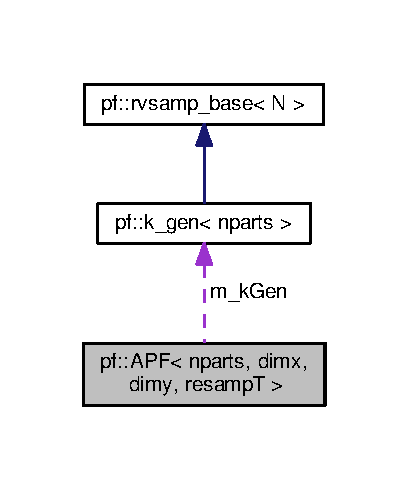
\includegraphics[width=196pt]{classpf_1_1APF__coll__graph}
\end{center}
\end{figure}
\subsection*{Public Types}
\begin{DoxyCompactItemize}
\item 
using \hyperlink{classpf_1_1APF_aa7fe7efd37dc23b06812aebdee256897}{ssv} = Eigen\+::\+Matrix$<$ double, dimx, 1 $>$
\item 
using \hyperlink{classpf_1_1APF_a852db242b5d02c58dc4e6a183a8cab65}{osv} = Eigen\+::\+Matrix$<$ double, dimy, 1 $>$
\item 
using \hyperlink{classpf_1_1APF_a771c0848fc35bf75e2d3f93bc4ee42ab}{Mat} = Eigen\+::\+Matrix$<$ double, dimx, dimx $>$
\item 
using \hyperlink{classpf_1_1APF_a4500221db97fe6af28b91fcc907bcc04}{array\+Double} = std\+::array$<$ double, nparts $>$
\item 
using \hyperlink{classpf_1_1APF_a62d28b3fa148d8f3fba03e4a1fb92b81}{array\+Vec} = std\+::array$<$ \hyperlink{classpf_1_1APF_aa7fe7efd37dc23b06812aebdee256897}{ssv}, nparts $>$
\item 
using \hyperlink{classpf_1_1APF_aca139948a9e7b0432afdcae7d2ffba01}{array\+U\+Int} = std\+::array$<$ unsigned int, nparts $>$
\end{DoxyCompactItemize}
\subsection*{Public Member Functions}
\begin{DoxyCompactItemize}
\item 
\hyperlink{classpf_1_1APF_a91c90bd5cd0703b03b1f157e09215ed2}{A\+PF} (const unsigned int \&rs=1)
\begin{DoxyCompactList}\small\item\em The constructor. \end{DoxyCompactList}\item 
double \hyperlink{classpf_1_1APF_a254e3d8de21bee812d89a3ad54aaebca}{get\+Log\+Cond\+Like} () const 
\begin{DoxyCompactList}\small\item\em Get the latest log conditional likelihood. \end{DoxyCompactList}\item 
std\+::vector$<$ \hyperlink{classpf_1_1APF_a771c0848fc35bf75e2d3f93bc4ee42ab}{Mat} $>$ \hyperlink{classpf_1_1APF_a2acc511dfc0ab4de6bfb7c44fb20023a}{get\+Expectations} () const 
\begin{DoxyCompactList}\small\item\em return all stored expectations (taken with respect to \$p(x\+\_\+t$\vert$y\+\_\+\{1\+:t\})\$ \end{DoxyCompactList}\item 
void \hyperlink{classpf_1_1APF_a060ab6fca79f677b89872274fd42e138}{filter} (const \hyperlink{classpf_1_1APF_a852db242b5d02c58dc4e6a183a8cab65}{osv} \&data, const std\+::vector$<$ std\+::function$<$ const \hyperlink{classpf_1_1APF_a771c0848fc35bf75e2d3f93bc4ee42ab}{Mat}(const \hyperlink{classpf_1_1APF_aa7fe7efd37dc23b06812aebdee256897}{ssv} \&)$>$ $>$ \&fs=std\+::vector$<$ std\+::function$<$ const \hyperlink{classpf_1_1APF_a771c0848fc35bf75e2d3f93bc4ee42ab}{Mat}(const \hyperlink{classpf_1_1APF_aa7fe7efd37dc23b06812aebdee256897}{ssv} \&)$>$ $>$())
\begin{DoxyCompactList}\small\item\em Use a new datapoint to update the filtering distribution (or smoothing if path\+Length $>$ 0). \end{DoxyCompactList}\item 
virtual double \hyperlink{classpf_1_1APF_a83b46eca3002716f355bf3cd29968433}{log\+Mu\+Ev} (const \hyperlink{classpf_1_1APF_aa7fe7efd37dc23b06812aebdee256897}{ssv} \&x1)=0
\begin{DoxyCompactList}\small\item\em Evaluates the log of mu. \end{DoxyCompactList}\item 
virtual \hyperlink{classpf_1_1APF_aa7fe7efd37dc23b06812aebdee256897}{ssv} \hyperlink{classpf_1_1APF_a25a1cba6c74c8c7e43d39fcca90a9fad}{prop\+Mu} (const \hyperlink{classpf_1_1APF_aa7fe7efd37dc23b06812aebdee256897}{ssv} \&xtm1)=0
\begin{DoxyCompactList}\small\item\em Evaluates the proposal distribution taking a Eigen\+::\+Matrix$<$double,dimx,1$>$ from the previous time\textquotesingle{}s state, and returning a state for the current time. \end{DoxyCompactList}\item 
virtual \hyperlink{classpf_1_1APF_aa7fe7efd37dc23b06812aebdee256897}{ssv} \hyperlink{classpf_1_1APF_a253087b9333ad8cbcd8cb9f21277bc48}{q1\+Samp} (const \hyperlink{classpf_1_1APF_a852db242b5d02c58dc4e6a183a8cab65}{osv} \&y1)=0
\begin{DoxyCompactList}\small\item\em Samples from q1. \end{DoxyCompactList}\item 
virtual \hyperlink{classpf_1_1APF_aa7fe7efd37dc23b06812aebdee256897}{ssv} \hyperlink{classpf_1_1APF_af99ef9dc1a78b32dafecb43e9f74d2a0}{f\+Samp} (const \hyperlink{classpf_1_1APF_aa7fe7efd37dc23b06812aebdee256897}{ssv} \&xtm1)=0
\begin{DoxyCompactList}\small\item\em Samples from f. \end{DoxyCompactList}\item 
virtual double \hyperlink{classpf_1_1APF_af706e40e1ccac9e36afc3fbd8cc515fd}{log\+Q1\+Ev} (const \hyperlink{classpf_1_1APF_aa7fe7efd37dc23b06812aebdee256897}{ssv} \&x1, const \hyperlink{classpf_1_1APF_a852db242b5d02c58dc4e6a183a8cab65}{osv} \&y1)=0
\begin{DoxyCompactList}\small\item\em Evaluates the log of q1. \end{DoxyCompactList}\item 
virtual double \hyperlink{classpf_1_1APF_a86a7cfd8ff411f8ed5f63d454c28afd2}{log\+G\+Ev} (const \hyperlink{classpf_1_1APF_a852db242b5d02c58dc4e6a183a8cab65}{osv} \&yt, const \hyperlink{classpf_1_1APF_aa7fe7efd37dc23b06812aebdee256897}{ssv} \&xt)=0
\begin{DoxyCompactList}\small\item\em Evaluates the log of g. \end{DoxyCompactList}\end{DoxyCompactItemize}
\subsection*{Protected Attributes}
\begin{DoxyCompactItemize}
\item 
std\+::array$<$ \hyperlink{classpf_1_1APF_aa7fe7efd37dc23b06812aebdee256897}{ssv}, nparts $>$ \hyperlink{classpf_1_1APF_a6e1188f48abcdc3baf7e3713e2748d7e}{m\+\_\+particles}\hypertarget{classpf_1_1APF_a6e1188f48abcdc3baf7e3713e2748d7e}{}\label{classpf_1_1APF_a6e1188f48abcdc3baf7e3713e2748d7e}

\begin{DoxyCompactList}\small\item\em particle samples \end{DoxyCompactList}\item 
std\+::array$<$ double, nparts $>$ \hyperlink{classpf_1_1APF_a4253879203914c206ec1af6a02e6fcb5}{m\+\_\+log\+Un\+Norm\+Weights}\hypertarget{classpf_1_1APF_a4253879203914c206ec1af6a02e6fcb5}{}\label{classpf_1_1APF_a4253879203914c206ec1af6a02e6fcb5}

\begin{DoxyCompactList}\small\item\em particle unnormalized weights \end{DoxyCompactList}\item 
unsigned int \hyperlink{classpf_1_1APF_af32e1254a52911cf1a890a3f64b30967}{m\+\_\+now}\hypertarget{classpf_1_1APF_af32e1254a52911cf1a890a3f64b30967}{}\label{classpf_1_1APF_af32e1254a52911cf1a890a3f64b30967}

\begin{DoxyCompactList}\small\item\em curren time \end{DoxyCompactList}\item 
double \hyperlink{classpf_1_1APF_a056d43b5cfea970fb7da090e969e4fef}{m\+\_\+log\+Last\+Cond\+Like}\hypertarget{classpf_1_1APF_a056d43b5cfea970fb7da090e969e4fef}{}\label{classpf_1_1APF_a056d43b5cfea970fb7da090e969e4fef}

\begin{DoxyCompactList}\small\item\em log p(y\+\_\+t$\vert$y\+\_\+\{1\+:t-\/1\}) or log p(y1) \end{DoxyCompactList}\item 
unsigned int \hyperlink{classpf_1_1APF_a81cf31027072208d3d7558c40adedeea}{m\+\_\+rs}\hypertarget{classpf_1_1APF_a81cf31027072208d3d7558c40adedeea}{}\label{classpf_1_1APF_a81cf31027072208d3d7558c40adedeea}

\begin{DoxyCompactList}\small\item\em the resampling schedule \end{DoxyCompactList}\item 
resampT \hyperlink{classpf_1_1APF_ab758c906000a3be70a1636a91676bfcc}{m\+\_\+resampler}\hypertarget{classpf_1_1APF_ab758c906000a3be70a1636a91676bfcc}{}\label{classpf_1_1APF_ab758c906000a3be70a1636a91676bfcc}

\begin{DoxyCompactList}\small\item\em resampler object (default ctor\textquotesingle{}d) \end{DoxyCompactList}\item 
\hyperlink{classpf_1_1k__gen}{k\+\_\+gen}$<$ nparts $>$ \hyperlink{classpf_1_1APF_a796dc4e376891c5199af5fbea8e7d068}{m\+\_\+k\+Gen}\hypertarget{classpf_1_1APF_a796dc4e376891c5199af5fbea8e7d068}{}\label{classpf_1_1APF_a796dc4e376891c5199af5fbea8e7d068}

\begin{DoxyCompactList}\small\item\em k generator object (default ctor\textquotesingle{}d) \end{DoxyCompactList}\item 
std\+::vector$<$ \hyperlink{classpf_1_1APF_a771c0848fc35bf75e2d3f93bc4ee42ab}{Mat} $>$ \hyperlink{classpf_1_1APF_ae63b91d0561efab0731fc31ad1065eca}{m\+\_\+expectations}\hypertarget{classpf_1_1APF_ae63b91d0561efab0731fc31ad1065eca}{}\label{classpf_1_1APF_ae63b91d0561efab0731fc31ad1065eca}

\begin{DoxyCompactList}\small\item\em expectations E\mbox{[}h(x\+\_\+t) $\vert$ y\+\_\+\{1\+:t\}\mbox{]} for user defined \char`\"{}h\char`\"{}s \end{DoxyCompactList}\end{DoxyCompactItemize}


\subsection{Detailed Description}
\subsubsection*{template$<$size\+\_\+t nparts, size\+\_\+t dimx, size\+\_\+t dimy, typename resampT$>$\\*
class pf\+::\+A\+P\+F$<$ nparts, dimx, dimy, resamp\+T $>$}

A base-\/class for Auxiliary Particle Filtering. Filtering only, no smoothing. 

\begin{DoxyAuthor}{Author}
taylor 
\end{DoxyAuthor}


\subsection{Member Typedef Documentation}
\index{pf\+::\+A\+PF@{pf\+::\+A\+PF}!array\+Double@{array\+Double}}
\index{array\+Double@{array\+Double}!pf\+::\+A\+PF@{pf\+::\+A\+PF}}
\subsubsection[{\texorpdfstring{array\+Double}{arrayDouble}}]{\setlength{\rightskip}{0pt plus 5cm}template$<$size\+\_\+t nparts, size\+\_\+t dimx, size\+\_\+t dimy, typename resampT $>$ using {\bf pf\+::\+A\+PF}$<$ nparts, dimx, dimy, resampT $>$\+::{\bf array\+Double} =  std\+::array$<$double, nparts$>$}\hypertarget{classpf_1_1APF_a4500221db97fe6af28b91fcc907bcc04}{}\label{classpf_1_1APF_a4500221db97fe6af28b91fcc907bcc04}
type alias for array of doubles \index{pf\+::\+A\+PF@{pf\+::\+A\+PF}!array\+U\+Int@{array\+U\+Int}}
\index{array\+U\+Int@{array\+U\+Int}!pf\+::\+A\+PF@{pf\+::\+A\+PF}}
\subsubsection[{\texorpdfstring{array\+U\+Int}{arrayUInt}}]{\setlength{\rightskip}{0pt plus 5cm}template$<$size\+\_\+t nparts, size\+\_\+t dimx, size\+\_\+t dimy, typename resampT $>$ using {\bf pf\+::\+A\+PF}$<$ nparts, dimx, dimy, resampT $>$\+::{\bf array\+U\+Int} =  std\+::array$<$unsigned int, nparts$>$}\hypertarget{classpf_1_1APF_aca139948a9e7b0432afdcae7d2ffba01}{}\label{classpf_1_1APF_aca139948a9e7b0432afdcae7d2ffba01}
type alias for array of unsigned ints \index{pf\+::\+A\+PF@{pf\+::\+A\+PF}!array\+Vec@{array\+Vec}}
\index{array\+Vec@{array\+Vec}!pf\+::\+A\+PF@{pf\+::\+A\+PF}}
\subsubsection[{\texorpdfstring{array\+Vec}{arrayVec}}]{\setlength{\rightskip}{0pt plus 5cm}template$<$size\+\_\+t nparts, size\+\_\+t dimx, size\+\_\+t dimy, typename resampT $>$ using {\bf pf\+::\+A\+PF}$<$ nparts, dimx, dimy, resampT $>$\+::{\bf array\+Vec} =  std\+::array$<${\bf ssv}, nparts$>$}\hypertarget{classpf_1_1APF_a62d28b3fa148d8f3fba03e4a1fb92b81}{}\label{classpf_1_1APF_a62d28b3fa148d8f3fba03e4a1fb92b81}
type alias for array of state vectors \index{pf\+::\+A\+PF@{pf\+::\+A\+PF}!Mat@{Mat}}
\index{Mat@{Mat}!pf\+::\+A\+PF@{pf\+::\+A\+PF}}
\subsubsection[{\texorpdfstring{Mat}{Mat}}]{\setlength{\rightskip}{0pt plus 5cm}template$<$size\+\_\+t nparts, size\+\_\+t dimx, size\+\_\+t dimy, typename resampT $>$ using {\bf pf\+::\+A\+PF}$<$ nparts, dimx, dimy, resampT $>$\+::{\bf Mat} =  Eigen\+::\+Matrix$<$double,dimx,dimx$>$}\hypertarget{classpf_1_1APF_a771c0848fc35bf75e2d3f93bc4ee42ab}{}\label{classpf_1_1APF_a771c0848fc35bf75e2d3f93bc4ee42ab}
type alias for linear algebra stuff (dimension of the state $^\wedge$2) \index{pf\+::\+A\+PF@{pf\+::\+A\+PF}!osv@{osv}}
\index{osv@{osv}!pf\+::\+A\+PF@{pf\+::\+A\+PF}}
\subsubsection[{\texorpdfstring{osv}{osv}}]{\setlength{\rightskip}{0pt plus 5cm}template$<$size\+\_\+t nparts, size\+\_\+t dimx, size\+\_\+t dimy, typename resampT $>$ using {\bf pf\+::\+A\+PF}$<$ nparts, dimx, dimy, resampT $>$\+::{\bf osv} =  Eigen\+::\+Matrix$<$double,dimy,1$>$}\hypertarget{classpf_1_1APF_a852db242b5d02c58dc4e6a183a8cab65}{}\label{classpf_1_1APF_a852db242b5d02c58dc4e6a183a8cab65}
\char`\"{}observation size vector\char`\"{} type alias for linear algebra stuff \index{pf\+::\+A\+PF@{pf\+::\+A\+PF}!ssv@{ssv}}
\index{ssv@{ssv}!pf\+::\+A\+PF@{pf\+::\+A\+PF}}
\subsubsection[{\texorpdfstring{ssv}{ssv}}]{\setlength{\rightskip}{0pt plus 5cm}template$<$size\+\_\+t nparts, size\+\_\+t dimx, size\+\_\+t dimy, typename resampT $>$ using {\bf pf\+::\+A\+PF}$<$ nparts, dimx, dimy, resampT $>$\+::{\bf ssv} =  Eigen\+::\+Matrix$<$double,dimx,1$>$}\hypertarget{classpf_1_1APF_aa7fe7efd37dc23b06812aebdee256897}{}\label{classpf_1_1APF_aa7fe7efd37dc23b06812aebdee256897}
\char`\"{}state size vector\char`\"{} type alias for linear algebra stuff 

\subsection{Constructor \& Destructor Documentation}
\index{pf\+::\+A\+PF@{pf\+::\+A\+PF}!A\+PF@{A\+PF}}
\index{A\+PF@{A\+PF}!pf\+::\+A\+PF@{pf\+::\+A\+PF}}
\subsubsection[{\texorpdfstring{A\+P\+F(const unsigned int \&rs=1)}{APF(const unsigned int &rs=1)}}]{\setlength{\rightskip}{0pt plus 5cm}template$<$size\+\_\+t nparts, size\+\_\+t dimx, size\+\_\+t dimy, typename resampT $>$ {\bf pf\+::\+A\+PF}$<$ nparts, dimx, dimy, resampT $>$\+::{\bf A\+PF} (
\begin{DoxyParamCaption}
\item[{const unsigned int \&}]{rs = {\ttfamily 1}}
\end{DoxyParamCaption}
)}\hypertarget{classpf_1_1APF_a91c90bd5cd0703b03b1f157e09215ed2}{}\label{classpf_1_1APF_a91c90bd5cd0703b03b1f157e09215ed2}


The constructor. 


\begin{DoxyParams}{Parameters}
{\em rs} & resampling schedule (e.\+g. resample every rs time points). \\
\hline
\end{DoxyParams}


\subsection{Member Function Documentation}
\index{pf\+::\+A\+PF@{pf\+::\+A\+PF}!filter@{filter}}
\index{filter@{filter}!pf\+::\+A\+PF@{pf\+::\+A\+PF}}
\subsubsection[{\texorpdfstring{filter(const osv \&data, const std\+::vector$<$ std\+::function$<$ const Mat(const ssv \&)$>$ $>$ \&fs=std\+::vector$<$ std\+::function$<$ const Mat(const ssv \&)$>$ $>$())}{filter(const osv &data, const std::vector< std::function< const Mat(const ssv &)> > &fs=std::vector< std::function< const Mat(const ssv &)> >())}}]{\setlength{\rightskip}{0pt plus 5cm}template$<$size\+\_\+t nparts, size\+\_\+t dimx, size\+\_\+t dimy, typename resampT $>$ void {\bf pf\+::\+A\+PF}$<$ nparts, dimx, dimy, resampT $>$\+::filter (
\begin{DoxyParamCaption}
\item[{const {\bf osv} \&}]{data, }
\item[{const std\+::vector$<$ std\+::function$<$ const {\bf Mat}(const {\bf ssv} \&)$>$ $>$ \&}]{fs = {\ttfamily std\+:\+:vector$<$std\+:\+:function$<$const~{\bf Mat}(const~{\bf ssv}\&)$>$~$>$()}}
\end{DoxyParamCaption}
)}\hypertarget{classpf_1_1APF_a060ab6fca79f677b89872274fd42e138}{}\label{classpf_1_1APF_a060ab6fca79f677b89872274fd42e138}


Use a new datapoint to update the filtering distribution (or smoothing if path\+Length $>$ 0). 


\begin{DoxyParams}{Parameters}
{\em data} & a Eigen\+::\+Matrix$<$double,dimy,1$>$ representing the data \\
\hline
{\em fs} & a std\+::vector of callback functions that are used to calculate expectations with respect to the filtering distribution. \\
\hline
\end{DoxyParams}
\index{pf\+::\+A\+PF@{pf\+::\+A\+PF}!f\+Samp@{f\+Samp}}
\index{f\+Samp@{f\+Samp}!pf\+::\+A\+PF@{pf\+::\+A\+PF}}
\subsubsection[{\texorpdfstring{f\+Samp(const ssv \&xtm1)=0}{fSamp(const ssv &xtm1)=0}}]{\setlength{\rightskip}{0pt plus 5cm}template$<$size\+\_\+t nparts, size\+\_\+t dimx, size\+\_\+t dimy, typename resampT $>$ virtual {\bf ssv} {\bf pf\+::\+A\+PF}$<$ nparts, dimx, dimy, resampT $>$\+::f\+Samp (
\begin{DoxyParamCaption}
\item[{const {\bf ssv} \&}]{xtm1}
\end{DoxyParamCaption}
)\hspace{0.3cm}{\ttfamily [pure virtual]}}\hypertarget{classpf_1_1APF_af99ef9dc1a78b32dafecb43e9f74d2a0}{}\label{classpf_1_1APF_af99ef9dc1a78b32dafecb43e9f74d2a0}


Samples from f. 


\begin{DoxyParams}{Parameters}
{\em xtm1} & a Eigen\+::\+Matrix$<$double,dimx,1$>$ representing the previous time\textquotesingle{}s state. \\
\hline
\end{DoxyParams}
\begin{DoxyReturn}{Returns}
a Eigen\+::\+Matrix$<$double,dimx,1$>$ state sample for the current time. 
\end{DoxyReturn}
\index{pf\+::\+A\+PF@{pf\+::\+A\+PF}!get\+Expectations@{get\+Expectations}}
\index{get\+Expectations@{get\+Expectations}!pf\+::\+A\+PF@{pf\+::\+A\+PF}}
\subsubsection[{\texorpdfstring{get\+Expectations() const }{getExpectations() const }}]{\setlength{\rightskip}{0pt plus 5cm}template$<$size\+\_\+t nparts, size\+\_\+t dimx, size\+\_\+t dimy, typename resampT $>$ auto {\bf pf\+::\+A\+PF}$<$ nparts, dimx, dimy, resampT $>$\+::get\+Expectations (
\begin{DoxyParamCaption}
{}
\end{DoxyParamCaption}
) const}\hypertarget{classpf_1_1APF_a2acc511dfc0ab4de6bfb7c44fb20023a}{}\label{classpf_1_1APF_a2acc511dfc0ab4de6bfb7c44fb20023a}


return all stored expectations (taken with respect to \$p(x\+\_\+t$\vert$y\+\_\+\{1\+:t\})\$ 

\begin{DoxyReturn}{Returns}
return a std\+::vector$<$\+Mat$>$ of expectations. How many depends on how many callbacks you gave to 
\end{DoxyReturn}
\index{pf\+::\+A\+PF@{pf\+::\+A\+PF}!get\+Log\+Cond\+Like@{get\+Log\+Cond\+Like}}
\index{get\+Log\+Cond\+Like@{get\+Log\+Cond\+Like}!pf\+::\+A\+PF@{pf\+::\+A\+PF}}
\subsubsection[{\texorpdfstring{get\+Log\+Cond\+Like() const }{getLogCondLike() const }}]{\setlength{\rightskip}{0pt plus 5cm}template$<$size\+\_\+t nparts, size\+\_\+t dimx, size\+\_\+t dimy, typename resampT $>$ double {\bf pf\+::\+A\+PF}$<$ nparts, dimx, dimy, resampT $>$\+::get\+Log\+Cond\+Like (
\begin{DoxyParamCaption}
{}
\end{DoxyParamCaption}
) const}\hypertarget{classpf_1_1APF_a254e3d8de21bee812d89a3ad54aaebca}{}\label{classpf_1_1APF_a254e3d8de21bee812d89a3ad54aaebca}


Get the latest log conditional likelihood. 

\begin{DoxyReturn}{Returns}
a double of the most recent conditional likelihood. 
\end{DoxyReturn}
\index{pf\+::\+A\+PF@{pf\+::\+A\+PF}!log\+G\+Ev@{log\+G\+Ev}}
\index{log\+G\+Ev@{log\+G\+Ev}!pf\+::\+A\+PF@{pf\+::\+A\+PF}}
\subsubsection[{\texorpdfstring{log\+G\+Ev(const osv \&yt, const ssv \&xt)=0}{logGEv(const osv &yt, const ssv &xt)=0}}]{\setlength{\rightskip}{0pt plus 5cm}template$<$size\+\_\+t nparts, size\+\_\+t dimx, size\+\_\+t dimy, typename resampT $>$ virtual double {\bf pf\+::\+A\+PF}$<$ nparts, dimx, dimy, resampT $>$\+::log\+G\+Ev (
\begin{DoxyParamCaption}
\item[{const {\bf osv} \&}]{yt, }
\item[{const {\bf ssv} \&}]{xt}
\end{DoxyParamCaption}
)\hspace{0.3cm}{\ttfamily [pure virtual]}}\hypertarget{classpf_1_1APF_a86a7cfd8ff411f8ed5f63d454c28afd2}{}\label{classpf_1_1APF_a86a7cfd8ff411f8ed5f63d454c28afd2}


Evaluates the log of g. 


\begin{DoxyParams}{Parameters}
{\em yt} & a Eigen\+::\+Matrix$<$double,dimy,1$>$ representing time t\textquotesingle{}s data observation. \\
\hline
{\em xt} & a Eigen\+::\+Matrix$<$double,dimx,1$>$ representing time t\textquotesingle{}s state. \\
\hline
\end{DoxyParams}
\begin{DoxyReturn}{Returns}
a double evaluation. 
\end{DoxyReturn}
\index{pf\+::\+A\+PF@{pf\+::\+A\+PF}!log\+Mu\+Ev@{log\+Mu\+Ev}}
\index{log\+Mu\+Ev@{log\+Mu\+Ev}!pf\+::\+A\+PF@{pf\+::\+A\+PF}}
\subsubsection[{\texorpdfstring{log\+Mu\+Ev(const ssv \&x1)=0}{logMuEv(const ssv &x1)=0}}]{\setlength{\rightskip}{0pt plus 5cm}template$<$size\+\_\+t nparts, size\+\_\+t dimx, size\+\_\+t dimy, typename resampT $>$ virtual double {\bf pf\+::\+A\+PF}$<$ nparts, dimx, dimy, resampT $>$\+::log\+Mu\+Ev (
\begin{DoxyParamCaption}
\item[{const {\bf ssv} \&}]{x1}
\end{DoxyParamCaption}
)\hspace{0.3cm}{\ttfamily [pure virtual]}}\hypertarget{classpf_1_1APF_a83b46eca3002716f355bf3cd29968433}{}\label{classpf_1_1APF_a83b46eca3002716f355bf3cd29968433}


Evaluates the log of mu. 


\begin{DoxyParams}{Parameters}
{\em x1} & a Eigen\+::\+Matrix$<$double,dimx,1$>$ representing time 1\textquotesingle{}s state. \\
\hline
\end{DoxyParams}
\begin{DoxyReturn}{Returns}
a double evaluation. 
\end{DoxyReturn}
\index{pf\+::\+A\+PF@{pf\+::\+A\+PF}!log\+Q1\+Ev@{log\+Q1\+Ev}}
\index{log\+Q1\+Ev@{log\+Q1\+Ev}!pf\+::\+A\+PF@{pf\+::\+A\+PF}}
\subsubsection[{\texorpdfstring{log\+Q1\+Ev(const ssv \&x1, const osv \&y1)=0}{logQ1Ev(const ssv &x1, const osv &y1)=0}}]{\setlength{\rightskip}{0pt plus 5cm}template$<$size\+\_\+t nparts, size\+\_\+t dimx, size\+\_\+t dimy, typename resampT $>$ virtual double {\bf pf\+::\+A\+PF}$<$ nparts, dimx, dimy, resampT $>$\+::log\+Q1\+Ev (
\begin{DoxyParamCaption}
\item[{const {\bf ssv} \&}]{x1, }
\item[{const {\bf osv} \&}]{y1}
\end{DoxyParamCaption}
)\hspace{0.3cm}{\ttfamily [pure virtual]}}\hypertarget{classpf_1_1APF_af706e40e1ccac9e36afc3fbd8cc515fd}{}\label{classpf_1_1APF_af706e40e1ccac9e36afc3fbd8cc515fd}


Evaluates the log of q1. 


\begin{DoxyParams}{Parameters}
{\em x1} & a Eigen\+::\+Matrix$<$double,dimx,1$>$ representing time 1\textquotesingle{}s state. \\
\hline
{\em y1} & a Eigen\+::\+Matrix$<$double,dimy,1$>$ representing time 1\textquotesingle{}s data observation. \\
\hline
\end{DoxyParams}
\begin{DoxyReturn}{Returns}
a double evaluation. 
\end{DoxyReturn}
\index{pf\+::\+A\+PF@{pf\+::\+A\+PF}!prop\+Mu@{prop\+Mu}}
\index{prop\+Mu@{prop\+Mu}!pf\+::\+A\+PF@{pf\+::\+A\+PF}}
\subsubsection[{\texorpdfstring{prop\+Mu(const ssv \&xtm1)=0}{propMu(const ssv &xtm1)=0}}]{\setlength{\rightskip}{0pt plus 5cm}template$<$size\+\_\+t nparts, size\+\_\+t dimx, size\+\_\+t dimy, typename resampT $>$ virtual {\bf ssv} {\bf pf\+::\+A\+PF}$<$ nparts, dimx, dimy, resampT $>$\+::prop\+Mu (
\begin{DoxyParamCaption}
\item[{const {\bf ssv} \&}]{xtm1}
\end{DoxyParamCaption}
)\hspace{0.3cm}{\ttfamily [pure virtual]}}\hypertarget{classpf_1_1APF_a25a1cba6c74c8c7e43d39fcca90a9fad}{}\label{classpf_1_1APF_a25a1cba6c74c8c7e43d39fcca90a9fad}


Evaluates the proposal distribution taking a Eigen\+::\+Matrix$<$double,dimx,1$>$ from the previous time\textquotesingle{}s state, and returning a state for the current time. 


\begin{DoxyParams}{Parameters}
{\em xtm1} & a Eigen\+::\+Matrix$<$double,dimx,1$>$ representing the previous time\textquotesingle{}s state. \\
\hline
\end{DoxyParams}
\begin{DoxyReturn}{Returns}
a Eigen\+::\+Matrix$<$double,dimx,1$>$ representing a likely current time state, to be used by the observation density. 
\end{DoxyReturn}
\index{pf\+::\+A\+PF@{pf\+::\+A\+PF}!q1\+Samp@{q1\+Samp}}
\index{q1\+Samp@{q1\+Samp}!pf\+::\+A\+PF@{pf\+::\+A\+PF}}
\subsubsection[{\texorpdfstring{q1\+Samp(const osv \&y1)=0}{q1Samp(const osv &y1)=0}}]{\setlength{\rightskip}{0pt plus 5cm}template$<$size\+\_\+t nparts, size\+\_\+t dimx, size\+\_\+t dimy, typename resampT $>$ virtual {\bf ssv} {\bf pf\+::\+A\+PF}$<$ nparts, dimx, dimy, resampT $>$\+::q1\+Samp (
\begin{DoxyParamCaption}
\item[{const {\bf osv} \&}]{y1}
\end{DoxyParamCaption}
)\hspace{0.3cm}{\ttfamily [pure virtual]}}\hypertarget{classpf_1_1APF_a253087b9333ad8cbcd8cb9f21277bc48}{}\label{classpf_1_1APF_a253087b9333ad8cbcd8cb9f21277bc48}


Samples from q1. 


\begin{DoxyParams}{Parameters}
{\em y1} & a Eigen\+::\+Matrix$<$double,dimy,1$>$ representing time 1\textquotesingle{}s data point. \\
\hline
\end{DoxyParams}
\begin{DoxyReturn}{Returns}
a Eigen\+::\+Matrix$<$double,dimx,1$>$ sample for time 1\textquotesingle{}s state. 
\end{DoxyReturn}


The documentation for this class was generated from the following file\+:\begin{DoxyCompactItemize}
\item 
include/\hyperlink{auxiliary__pf_8h}{auxiliary\+\_\+pf.\+h}\end{DoxyCompactItemize}

\hypertarget{classpf_1_1BSFilter}{}\section{pf\+:\+:B\+S\+Filter$<$ nparts, dimx, dimy, resampT $>$ Class Template Reference}
\label{classpf_1_1BSFilter}\index{pf\+::\+B\+S\+Filter$<$ nparts, dimx, dimy, resamp\+T $>$@{pf\+::\+B\+S\+Filter$<$ nparts, dimx, dimy, resamp\+T $>$}}


A base class for the boostrap particle filter.  




{\ttfamily \#include $<$bootstrap\+\_\+filter.\+h$>$}

\subsection*{Public Types}
\begin{DoxyCompactItemize}
\item 
using \hyperlink{classpf_1_1BSFilter_a95fa891a3af39cb14cfe8521fb1d0f88}{ssv} = Eigen\+::\+Matrix$<$ double, dimx, 1 $>$
\item 
using \hyperlink{classpf_1_1BSFilter_a46aaa88331b87e69ad3d1fcdc3b1db4e}{osv} = Eigen\+::\+Matrix$<$ double, dimy, 1 $>$
\item 
using \hyperlink{classpf_1_1BSFilter_a0fea63439948d095468ec14792abb396}{Mat} = Eigen\+::\+Matrix$<$ double, dimx, dimx $>$
\item 
using \hyperlink{classpf_1_1BSFilter_a567bc3c2a16c2a6f8b4673fe88ebbfda}{array\+States} = std\+::array$<$ \hyperlink{classpf_1_1BSFilter_a95fa891a3af39cb14cfe8521fb1d0f88}{ssv}, nparts $>$
\item 
using \hyperlink{classpf_1_1BSFilter_a770a16204c3c328cc15c5822f4687a8b}{array\+Double} = std\+::array$<$ double, nparts $>$
\end{DoxyCompactItemize}
\subsection*{Public Member Functions}
\begin{DoxyCompactItemize}
\item 
\hyperlink{classpf_1_1BSFilter_aca64b4c5d1bcc805aecb261b40203a04}{B\+S\+Filter} (const unsigned int \&rs=1)
\begin{DoxyCompactList}\small\item\em The constructor. \end{DoxyCompactList}\item 
double \hyperlink{classpf_1_1BSFilter_a72063c3e2e09f1fefb29563c1929a490}{get\+Log\+Cond\+Like} () const 
\begin{DoxyCompactList}\small\item\em Returns the most recent (log-\/) conditiona likelihood. \end{DoxyCompactList}\item 
void \hyperlink{classpf_1_1BSFilter_ab3e3a45671cb71e473a5bf6d6c363d9c}{filter} (const \hyperlink{classpf_1_1BSFilter_a46aaa88331b87e69ad3d1fcdc3b1db4e}{osv} \&data, const std\+::vector$<$ std\+::function$<$ const \hyperlink{classpf_1_1BSFilter_a0fea63439948d095468ec14792abb396}{Mat}(const \hyperlink{classpf_1_1BSFilter_a95fa891a3af39cb14cfe8521fb1d0f88}{ssv} \&)$>$ $>$ \&fs=std\+::vector$<$ std\+::function$<$ const \hyperlink{classpf_1_1BSFilter_a0fea63439948d095468ec14792abb396}{Mat}(const \hyperlink{classpf_1_1BSFilter_a95fa891a3af39cb14cfe8521fb1d0f88}{ssv} \&)$>$ $>$())
\begin{DoxyCompactList}\small\item\em updates filtering distribution on a new datapoint. Optionally stores expectations of functionals. \end{DoxyCompactList}\item 
auto \hyperlink{classpf_1_1BSFilter_affea414129ce50176ab0f873d5339e18}{get\+Expectations} () const -\/$>$ std\+::vector$<$ \hyperlink{classpf_1_1BSFilter_a0fea63439948d095468ec14792abb396}{Mat} $>$
\begin{DoxyCompactList}\small\item\em return all stored expectations (taken with respect to \$p(x\+\_\+t$\vert$y\+\_\+\{1\+:t\})\$ \end{DoxyCompactList}\item 
virtual double \hyperlink{classpf_1_1BSFilter_a1806a607fed9163427207cc7eb21e2dd}{log\+Mu\+Ev} (const \hyperlink{classpf_1_1BSFilter_a95fa891a3af39cb14cfe8521fb1d0f88}{ssv} \&x1)=0
\begin{DoxyCompactList}\small\item\em Calculate mu\+Ev or logmu\+Ev. \end{DoxyCompactList}\item 
virtual \hyperlink{classpf_1_1BSFilter_a95fa891a3af39cb14cfe8521fb1d0f88}{ssv} \hyperlink{classpf_1_1BSFilter_aa6079ca23980bd4dc98378a88297b4bd}{q1\+Samp} (const \hyperlink{classpf_1_1BSFilter_a46aaa88331b87e69ad3d1fcdc3b1db4e}{osv} \&y1)=0
\begin{DoxyCompactList}\small\item\em Samples from time 1 proposal. \end{DoxyCompactList}\item 
virtual double \hyperlink{classpf_1_1BSFilter_a00509b44e9beb183b9f5b5b61ff6b5a3}{log\+Q1\+Ev} (const \hyperlink{classpf_1_1BSFilter_a95fa891a3af39cb14cfe8521fb1d0f88}{ssv} \&x1, const \hyperlink{classpf_1_1BSFilter_a46aaa88331b87e69ad3d1fcdc3b1db4e}{osv} \&y1)=0
\begin{DoxyCompactList}\small\item\em Calculate q1\+Ev or log q1\+Ev. \end{DoxyCompactList}\item 
virtual double \hyperlink{classpf_1_1BSFilter_a2c4dd5363a48e218e8e83024696f586b}{log\+G\+Ev} (const \hyperlink{classpf_1_1BSFilter_a46aaa88331b87e69ad3d1fcdc3b1db4e}{osv} \&yt, const \hyperlink{classpf_1_1BSFilter_a95fa891a3af39cb14cfe8521fb1d0f88}{ssv} \&xt)=0
\begin{DoxyCompactList}\small\item\em Calculate g\+Ev or log\+G\+Ev. \end{DoxyCompactList}\item 
virtual \hyperlink{classpf_1_1BSFilter_a95fa891a3af39cb14cfe8521fb1d0f88}{ssv} \hyperlink{classpf_1_1BSFilter_a56c232aa4d91895ea3c69dff65c6d20e}{f\+Samp} (const \hyperlink{classpf_1_1BSFilter_a95fa891a3af39cb14cfe8521fb1d0f88}{ssv} \&xtm1)=0
\begin{DoxyCompactList}\small\item\em Sample from the state transition distribution. \end{DoxyCompactList}\end{DoxyCompactItemize}
\subsection*{Protected Attributes}
\begin{DoxyCompactItemize}
\item 
\hyperlink{classpf_1_1BSFilter_a567bc3c2a16c2a6f8b4673fe88ebbfda}{array\+States} \hyperlink{classpf_1_1BSFilter_ad341fdcb4318d771a4678dbfcf991d93}{m\+\_\+particles}\hypertarget{classpf_1_1BSFilter_ad341fdcb4318d771a4678dbfcf991d93}{}\label{classpf_1_1BSFilter_ad341fdcb4318d771a4678dbfcf991d93}

\begin{DoxyCompactList}\small\item\em particle samples \end{DoxyCompactList}\item 
\hyperlink{classpf_1_1BSFilter_a770a16204c3c328cc15c5822f4687a8b}{array\+Double} \hyperlink{classpf_1_1BSFilter_a0baebf18dfe1ae125394836d60fda864}{m\+\_\+log\+Un\+Norm\+Weights}\hypertarget{classpf_1_1BSFilter_a0baebf18dfe1ae125394836d60fda864}{}\label{classpf_1_1BSFilter_a0baebf18dfe1ae125394836d60fda864}

\begin{DoxyCompactList}\small\item\em particle unnormalized weights \end{DoxyCompactList}\item 
unsigned int \hyperlink{classpf_1_1BSFilter_ab0b52326557233e6ed24015150b38e6f}{m\+\_\+now}\hypertarget{classpf_1_1BSFilter_ab0b52326557233e6ed24015150b38e6f}{}\label{classpf_1_1BSFilter_ab0b52326557233e6ed24015150b38e6f}

\begin{DoxyCompactList}\small\item\em time point \end{DoxyCompactList}\item 
double \hyperlink{classpf_1_1BSFilter_ac990cd2c5fd4f80211c8056440f1b10e}{m\+\_\+log\+Last\+Cond\+Like}\hypertarget{classpf_1_1BSFilter_ac990cd2c5fd4f80211c8056440f1b10e}{}\label{classpf_1_1BSFilter_ac990cd2c5fd4f80211c8056440f1b10e}

\begin{DoxyCompactList}\small\item\em log p(y\+\_\+t$\vert$y\+\_\+\{1\+:t-\/1\}) or log p(y1) \end{DoxyCompactList}\item 
resampT \hyperlink{classpf_1_1BSFilter_a3f63885229a23791df71aa43e81b5aae}{m\+\_\+resampler}\hypertarget{classpf_1_1BSFilter_a3f63885229a23791df71aa43e81b5aae}{}\label{classpf_1_1BSFilter_a3f63885229a23791df71aa43e81b5aae}

\begin{DoxyCompactList}\small\item\em resampler object \end{DoxyCompactList}\item 
std\+::vector$<$ \hyperlink{classpf_1_1BSFilter_a0fea63439948d095468ec14792abb396}{Mat} $>$ \hyperlink{classpf_1_1BSFilter_abdddf9da762b8b5454ddb98bbfba53d6}{m\+\_\+expectations}\hypertarget{classpf_1_1BSFilter_abdddf9da762b8b5454ddb98bbfba53d6}{}\label{classpf_1_1BSFilter_abdddf9da762b8b5454ddb98bbfba53d6}

\begin{DoxyCompactList}\small\item\em expectations E\mbox{[}h(x\+\_\+t) $\vert$ y\+\_\+\{1\+:t\}\mbox{]} for user defined \char`\"{}h\char`\"{}s \end{DoxyCompactList}\item 
unsigned int \hyperlink{classpf_1_1BSFilter_a8bf45df72ff688f972ef77cf199bfda1}{m\+\_\+resamp\+Sched}\hypertarget{classpf_1_1BSFilter_a8bf45df72ff688f972ef77cf199bfda1}{}\label{classpf_1_1BSFilter_a8bf45df72ff688f972ef77cf199bfda1}

\begin{DoxyCompactList}\small\item\em resampling schedule (e.\+g. resample every \+\_\+\+\_\+ time points) \end{DoxyCompactList}\end{DoxyCompactItemize}


\subsection{Detailed Description}
\subsubsection*{template$<$size\+\_\+t nparts, size\+\_\+t dimx, size\+\_\+t dimy, typename resampT$>$\\*
class pf\+::\+B\+S\+Filter$<$ nparts, dimx, dimy, resamp\+T $>$}

A base class for the boostrap particle filter. 

\begin{DoxyAuthor}{Author}
taylor 
\end{DoxyAuthor}


\subsection{Member Typedef Documentation}
\index{pf\+::\+B\+S\+Filter@{pf\+::\+B\+S\+Filter}!array\+Double@{array\+Double}}
\index{array\+Double@{array\+Double}!pf\+::\+B\+S\+Filter@{pf\+::\+B\+S\+Filter}}
\subsubsection[{\texorpdfstring{array\+Double}{arrayDouble}}]{\setlength{\rightskip}{0pt plus 5cm}template$<$size\+\_\+t nparts, size\+\_\+t dimx, size\+\_\+t dimy, typename resampT $>$ using {\bf pf\+::\+B\+S\+Filter}$<$ nparts, dimx, dimy, resampT $>$\+::{\bf array\+Double} =  std\+::array$<$double, nparts$>$}\hypertarget{classpf_1_1BSFilter_a770a16204c3c328cc15c5822f4687a8b}{}\label{classpf_1_1BSFilter_a770a16204c3c328cc15c5822f4687a8b}
type alias for array of doubles \index{pf\+::\+B\+S\+Filter@{pf\+::\+B\+S\+Filter}!array\+States@{array\+States}}
\index{array\+States@{array\+States}!pf\+::\+B\+S\+Filter@{pf\+::\+B\+S\+Filter}}
\subsubsection[{\texorpdfstring{array\+States}{arrayStates}}]{\setlength{\rightskip}{0pt plus 5cm}template$<$size\+\_\+t nparts, size\+\_\+t dimx, size\+\_\+t dimy, typename resampT $>$ using {\bf pf\+::\+B\+S\+Filter}$<$ nparts, dimx, dimy, resampT $>$\+::{\bf array\+States} =  std\+::array$<${\bf ssv}, nparts$>$}\hypertarget{classpf_1_1BSFilter_a567bc3c2a16c2a6f8b4673fe88ebbfda}{}\label{classpf_1_1BSFilter_a567bc3c2a16c2a6f8b4673fe88ebbfda}
type alias for linear algebra stuff \index{pf\+::\+B\+S\+Filter@{pf\+::\+B\+S\+Filter}!Mat@{Mat}}
\index{Mat@{Mat}!pf\+::\+B\+S\+Filter@{pf\+::\+B\+S\+Filter}}
\subsubsection[{\texorpdfstring{Mat}{Mat}}]{\setlength{\rightskip}{0pt plus 5cm}template$<$size\+\_\+t nparts, size\+\_\+t dimx, size\+\_\+t dimy, typename resampT $>$ using {\bf pf\+::\+B\+S\+Filter}$<$ nparts, dimx, dimy, resampT $>$\+::{\bf Mat} =  Eigen\+::\+Matrix$<$double, dimx, dimx$>$}\hypertarget{classpf_1_1BSFilter_a0fea63439948d095468ec14792abb396}{}\label{classpf_1_1BSFilter_a0fea63439948d095468ec14792abb396}
type alias for linear algebra stuff \index{pf\+::\+B\+S\+Filter@{pf\+::\+B\+S\+Filter}!osv@{osv}}
\index{osv@{osv}!pf\+::\+B\+S\+Filter@{pf\+::\+B\+S\+Filter}}
\subsubsection[{\texorpdfstring{osv}{osv}}]{\setlength{\rightskip}{0pt plus 5cm}template$<$size\+\_\+t nparts, size\+\_\+t dimx, size\+\_\+t dimy, typename resampT $>$ using {\bf pf\+::\+B\+S\+Filter}$<$ nparts, dimx, dimy, resampT $>$\+::{\bf osv} =  Eigen\+::\+Matrix$<$double, dimy, 1$>$}\hypertarget{classpf_1_1BSFilter_a46aaa88331b87e69ad3d1fcdc3b1db4e}{}\label{classpf_1_1BSFilter_a46aaa88331b87e69ad3d1fcdc3b1db4e}
\char`\"{}obs size vector\char`\"{} type alias for linear algebra stuff \index{pf\+::\+B\+S\+Filter@{pf\+::\+B\+S\+Filter}!ssv@{ssv}}
\index{ssv@{ssv}!pf\+::\+B\+S\+Filter@{pf\+::\+B\+S\+Filter}}
\subsubsection[{\texorpdfstring{ssv}{ssv}}]{\setlength{\rightskip}{0pt plus 5cm}template$<$size\+\_\+t nparts, size\+\_\+t dimx, size\+\_\+t dimy, typename resampT $>$ using {\bf pf\+::\+B\+S\+Filter}$<$ nparts, dimx, dimy, resampT $>$\+::{\bf ssv} =  Eigen\+::\+Matrix$<$double, dimx, 1$>$}\hypertarget{classpf_1_1BSFilter_a95fa891a3af39cb14cfe8521fb1d0f88}{}\label{classpf_1_1BSFilter_a95fa891a3af39cb14cfe8521fb1d0f88}
\char`\"{}state size vector\char`\"{} type alias for linear algebra stuff 

\subsection{Constructor \& Destructor Documentation}
\index{pf\+::\+B\+S\+Filter@{pf\+::\+B\+S\+Filter}!B\+S\+Filter@{B\+S\+Filter}}
\index{B\+S\+Filter@{B\+S\+Filter}!pf\+::\+B\+S\+Filter@{pf\+::\+B\+S\+Filter}}
\subsubsection[{\texorpdfstring{B\+S\+Filter(const unsigned int \&rs=1)}{BSFilter(const unsigned int &rs=1)}}]{\setlength{\rightskip}{0pt plus 5cm}template$<$size\+\_\+t nparts, size\+\_\+t dimx, size\+\_\+t dimy, typename resampT $>$ {\bf pf\+::\+B\+S\+Filter}$<$ nparts, dimx, dimy, resampT $>$\+::{\bf B\+S\+Filter} (
\begin{DoxyParamCaption}
\item[{const unsigned int \&}]{rs = {\ttfamily 1}}
\end{DoxyParamCaption}
)}\hypertarget{classpf_1_1BSFilter_aca64b4c5d1bcc805aecb261b40203a04}{}\label{classpf_1_1BSFilter_aca64b4c5d1bcc805aecb261b40203a04}


The constructor. 


\begin{DoxyParams}{Parameters}
{\em rs} & the resampling schedule (e.\+g. every rs time point) \\
\hline
\end{DoxyParams}


\subsection{Member Function Documentation}
\index{pf\+::\+B\+S\+Filter@{pf\+::\+B\+S\+Filter}!filter@{filter}}
\index{filter@{filter}!pf\+::\+B\+S\+Filter@{pf\+::\+B\+S\+Filter}}
\subsubsection[{\texorpdfstring{filter(const osv \&data, const std\+::vector$<$ std\+::function$<$ const Mat(const ssv \&)$>$ $>$ \&fs=std\+::vector$<$ std\+::function$<$ const Mat(const ssv \&)$>$ $>$())}{filter(const osv &data, const std::vector< std::function< const Mat(const ssv &)> > &fs=std::vector< std::function< const Mat(const ssv &)> >())}}]{\setlength{\rightskip}{0pt plus 5cm}template$<$size\+\_\+t nparts, size\+\_\+t dimx, size\+\_\+t dimy, typename resampT $>$ void {\bf pf\+::\+B\+S\+Filter}$<$ nparts, dimx, dimy, resampT $>$\+::filter (
\begin{DoxyParamCaption}
\item[{const {\bf osv} \&}]{data, }
\item[{const std\+::vector$<$ std\+::function$<$ const {\bf Mat}(const {\bf ssv} \&)$>$ $>$ \&}]{fs = {\ttfamily std\+:\+:vector$<$std\+:\+:function$<$const~{\bf Mat}(const~{\bf ssv}\&)$>$~$>$()}}
\end{DoxyParamCaption}
)}\hypertarget{classpf_1_1BSFilter_ab3e3a45671cb71e473a5bf6d6c363d9c}{}\label{classpf_1_1BSFilter_ab3e3a45671cb71e473a5bf6d6c363d9c}


updates filtering distribution on a new datapoint. Optionally stores expectations of functionals. 


\begin{DoxyParams}{Parameters}
{\em data} & the most recent data point \\
\hline
{\em fs} & a vector of functions if you want to calculate expectations. \\
\hline
\end{DoxyParams}
\begin{DoxyRefDesc}{Todo}
\item[\hyperlink{todo__todo000001}{Todo}]\+: work in support for effective sample size stuff. \end{DoxyRefDesc}
\index{pf\+::\+B\+S\+Filter@{pf\+::\+B\+S\+Filter}!f\+Samp@{f\+Samp}}
\index{f\+Samp@{f\+Samp}!pf\+::\+B\+S\+Filter@{pf\+::\+B\+S\+Filter}}
\subsubsection[{\texorpdfstring{f\+Samp(const ssv \&xtm1)=0}{fSamp(const ssv &xtm1)=0}}]{\setlength{\rightskip}{0pt plus 5cm}template$<$size\+\_\+t nparts, size\+\_\+t dimx, size\+\_\+t dimy, typename resampT $>$ virtual {\bf ssv} {\bf pf\+::\+B\+S\+Filter}$<$ nparts, dimx, dimy, resampT $>$\+::f\+Samp (
\begin{DoxyParamCaption}
\item[{const {\bf ssv} \&}]{xtm1}
\end{DoxyParamCaption}
)\hspace{0.3cm}{\ttfamily [pure virtual]}}\hypertarget{classpf_1_1BSFilter_a56c232aa4d91895ea3c69dff65c6d20e}{}\label{classpf_1_1BSFilter_a56c232aa4d91895ea3c69dff65c6d20e}


Sample from the state transition distribution. 


\begin{DoxyParams}{Parameters}
{\em xtm1} & is a const Vec\& describing the time t-\/1 state \\
\hline
\end{DoxyParams}
\begin{DoxyReturn}{Returns}
the sample as a Vec 
\end{DoxyReturn}
\index{pf\+::\+B\+S\+Filter@{pf\+::\+B\+S\+Filter}!get\+Expectations@{get\+Expectations}}
\index{get\+Expectations@{get\+Expectations}!pf\+::\+B\+S\+Filter@{pf\+::\+B\+S\+Filter}}
\subsubsection[{\texorpdfstring{get\+Expectations() const -\/$>$ std\+::vector$<$ Mat $>$}{getExpectations() const -> std::vector< Mat >}}]{\setlength{\rightskip}{0pt plus 5cm}template$<$size\+\_\+t nparts, size\+\_\+t dimx, size\+\_\+t dimy, typename resampT $>$ auto {\bf pf\+::\+B\+S\+Filter}$<$ nparts, dimx, dimy, resampT $>$\+::get\+Expectations (
\begin{DoxyParamCaption}
{}
\end{DoxyParamCaption}
) const -\/$>$ std\+::vector$<${\bf Mat}$>$}\hypertarget{classpf_1_1BSFilter_affea414129ce50176ab0f873d5339e18}{}\label{classpf_1_1BSFilter_affea414129ce50176ab0f873d5339e18}


return all stored expectations (taken with respect to \$p(x\+\_\+t$\vert$y\+\_\+\{1\+:t\})\$ 

\begin{DoxyReturn}{Returns}
return a std\+::vector$<$\+Mat$>$ of expectations. How many depends on how many callbacks you gave to 
\end{DoxyReturn}
\index{pf\+::\+B\+S\+Filter@{pf\+::\+B\+S\+Filter}!get\+Log\+Cond\+Like@{get\+Log\+Cond\+Like}}
\index{get\+Log\+Cond\+Like@{get\+Log\+Cond\+Like}!pf\+::\+B\+S\+Filter@{pf\+::\+B\+S\+Filter}}
\subsubsection[{\texorpdfstring{get\+Log\+Cond\+Like() const }{getLogCondLike() const }}]{\setlength{\rightskip}{0pt plus 5cm}template$<$size\+\_\+t nparts, size\+\_\+t dimx, size\+\_\+t dimy, typename resampT $>$ double {\bf pf\+::\+B\+S\+Filter}$<$ nparts, dimx, dimy, resampT $>$\+::get\+Log\+Cond\+Like (
\begin{DoxyParamCaption}
{}
\end{DoxyParamCaption}
) const}\hypertarget{classpf_1_1BSFilter_a72063c3e2e09f1fefb29563c1929a490}{}\label{classpf_1_1BSFilter_a72063c3e2e09f1fefb29563c1929a490}


Returns the most recent (log-\/) conditiona likelihood. 

\begin{DoxyReturn}{Returns}
log p(y\+\_\+t $\vert$ y\+\_\+\{1\+:t-\/1\}) 
\end{DoxyReturn}
\index{pf\+::\+B\+S\+Filter@{pf\+::\+B\+S\+Filter}!log\+G\+Ev@{log\+G\+Ev}}
\index{log\+G\+Ev@{log\+G\+Ev}!pf\+::\+B\+S\+Filter@{pf\+::\+B\+S\+Filter}}
\subsubsection[{\texorpdfstring{log\+G\+Ev(const osv \&yt, const ssv \&xt)=0}{logGEv(const osv &yt, const ssv &xt)=0}}]{\setlength{\rightskip}{0pt plus 5cm}template$<$size\+\_\+t nparts, size\+\_\+t dimx, size\+\_\+t dimy, typename resampT $>$ virtual double {\bf pf\+::\+B\+S\+Filter}$<$ nparts, dimx, dimy, resampT $>$\+::log\+G\+Ev (
\begin{DoxyParamCaption}
\item[{const {\bf osv} \&}]{yt, }
\item[{const {\bf ssv} \&}]{xt}
\end{DoxyParamCaption}
)\hspace{0.3cm}{\ttfamily [pure virtual]}}\hypertarget{classpf_1_1BSFilter_a2c4dd5363a48e218e8e83024696f586b}{}\label{classpf_1_1BSFilter_a2c4dd5363a48e218e8e83024696f586b}


Calculate g\+Ev or log\+G\+Ev. 


\begin{DoxyParams}{Parameters}
{\em yt} & is a const Vec\& describing the time t datum \\
\hline
{\em xt} & is a const Vec\& describing the time t state \\
\hline
\end{DoxyParams}
\begin{DoxyReturn}{Returns}
the density or log-\/density evaluation as a double 
\end{DoxyReturn}
\index{pf\+::\+B\+S\+Filter@{pf\+::\+B\+S\+Filter}!log\+Mu\+Ev@{log\+Mu\+Ev}}
\index{log\+Mu\+Ev@{log\+Mu\+Ev}!pf\+::\+B\+S\+Filter@{pf\+::\+B\+S\+Filter}}
\subsubsection[{\texorpdfstring{log\+Mu\+Ev(const ssv \&x1)=0}{logMuEv(const ssv &x1)=0}}]{\setlength{\rightskip}{0pt plus 5cm}template$<$size\+\_\+t nparts, size\+\_\+t dimx, size\+\_\+t dimy, typename resampT $>$ virtual double {\bf pf\+::\+B\+S\+Filter}$<$ nparts, dimx, dimy, resampT $>$\+::log\+Mu\+Ev (
\begin{DoxyParamCaption}
\item[{const {\bf ssv} \&}]{x1}
\end{DoxyParamCaption}
)\hspace{0.3cm}{\ttfamily [pure virtual]}}\hypertarget{classpf_1_1BSFilter_a1806a607fed9163427207cc7eb21e2dd}{}\label{classpf_1_1BSFilter_a1806a607fed9163427207cc7eb21e2dd}


Calculate mu\+Ev or logmu\+Ev. 


\begin{DoxyParams}{Parameters}
{\em x1} & is a const Vec\& describing the state sample \\
\hline
\end{DoxyParams}
\begin{DoxyReturn}{Returns}
the density or log-\/density evaluation as a double 
\end{DoxyReturn}
\index{pf\+::\+B\+S\+Filter@{pf\+::\+B\+S\+Filter}!log\+Q1\+Ev@{log\+Q1\+Ev}}
\index{log\+Q1\+Ev@{log\+Q1\+Ev}!pf\+::\+B\+S\+Filter@{pf\+::\+B\+S\+Filter}}
\subsubsection[{\texorpdfstring{log\+Q1\+Ev(const ssv \&x1, const osv \&y1)=0}{logQ1Ev(const ssv &x1, const osv &y1)=0}}]{\setlength{\rightskip}{0pt plus 5cm}template$<$size\+\_\+t nparts, size\+\_\+t dimx, size\+\_\+t dimy, typename resampT $>$ virtual double {\bf pf\+::\+B\+S\+Filter}$<$ nparts, dimx, dimy, resampT $>$\+::log\+Q1\+Ev (
\begin{DoxyParamCaption}
\item[{const {\bf ssv} \&}]{x1, }
\item[{const {\bf osv} \&}]{y1}
\end{DoxyParamCaption}
)\hspace{0.3cm}{\ttfamily [pure virtual]}}\hypertarget{classpf_1_1BSFilter_a00509b44e9beb183b9f5b5b61ff6b5a3}{}\label{classpf_1_1BSFilter_a00509b44e9beb183b9f5b5b61ff6b5a3}


Calculate q1\+Ev or log q1\+Ev. 


\begin{DoxyParams}{Parameters}
{\em x1} & is a const Vec\& describing the time 1 state sample \\
\hline
{\em y1} & is a const Vec\& describing the time 1 datum \\
\hline
\end{DoxyParams}
\begin{DoxyReturn}{Returns}
the density or log-\/density evaluation as a double 
\end{DoxyReturn}
\index{pf\+::\+B\+S\+Filter@{pf\+::\+B\+S\+Filter}!q1\+Samp@{q1\+Samp}}
\index{q1\+Samp@{q1\+Samp}!pf\+::\+B\+S\+Filter@{pf\+::\+B\+S\+Filter}}
\subsubsection[{\texorpdfstring{q1\+Samp(const osv \&y1)=0}{q1Samp(const osv &y1)=0}}]{\setlength{\rightskip}{0pt plus 5cm}template$<$size\+\_\+t nparts, size\+\_\+t dimx, size\+\_\+t dimy, typename resampT $>$ virtual {\bf ssv} {\bf pf\+::\+B\+S\+Filter}$<$ nparts, dimx, dimy, resampT $>$\+::q1\+Samp (
\begin{DoxyParamCaption}
\item[{const {\bf osv} \&}]{y1}
\end{DoxyParamCaption}
)\hspace{0.3cm}{\ttfamily [pure virtual]}}\hypertarget{classpf_1_1BSFilter_aa6079ca23980bd4dc98378a88297b4bd}{}\label{classpf_1_1BSFilter_aa6079ca23980bd4dc98378a88297b4bd}


Samples from time 1 proposal. 


\begin{DoxyParams}{Parameters}
{\em y1} & is a const Vec\& representing the first observed datum \\
\hline
\end{DoxyParams}
\begin{DoxyReturn}{Returns}
the sample as a Vec 
\end{DoxyReturn}


The documentation for this class was generated from the following file\+:\begin{DoxyCompactItemize}
\item 
include/\hyperlink{bootstrap__filter_8h}{bootstrap\+\_\+filter.\+h}\end{DoxyCompactItemize}

\hypertarget{classpf_1_1cf__filter}{}\section{pf\+:\+:cf\+\_\+filter$<$ dimstate, dimobs $>$ Class Template Reference}
\label{classpf_1_1cf__filter}\index{pf\+::cf\+\_\+filter$<$ dimstate, dimobs $>$@{pf\+::cf\+\_\+filter$<$ dimstate, dimobs $>$}}


Abstract Base Class for Kalman filter and H\+MM filter.  




{\ttfamily \#include $<$cf\+\_\+filters.\+h$>$}



Inheritance diagram for pf\+:\+:cf\+\_\+filter$<$ dimstate, dimobs $>$\+:
\nopagebreak
\begin{figure}[H]
\begin{center}
\leavevmode
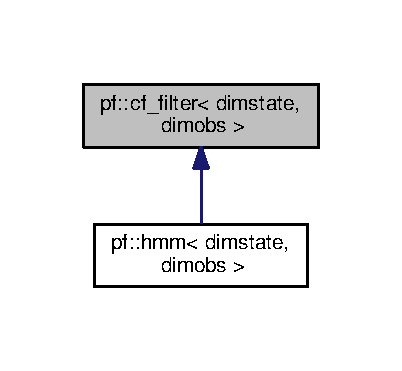
\includegraphics[width=193pt]{classpf_1_1cf__filter__inherit__graph}
\end{center}
\end{figure}
\subsection*{Public Types}
\begin{DoxyCompactItemize}
\item 
using \hyperlink{classpf_1_1cf__filter_a448f675e130ac4b340e2c3e545673d0d}{ssv} = Eigen\+::\+Matrix$<$ double, dimstate, 1 $>$
\item 
using \hyperlink{classpf_1_1cf__filter_ace17376128bb73ee73ff1b5c4972b317}{osv} = Eigen\+::\+Matrix$<$ double, dimstate, 1 $>$
\end{DoxyCompactItemize}
\subsection*{Public Member Functions}
\begin{DoxyCompactItemize}
\item 
virtual double \hyperlink{classpf_1_1cf__filter_ad9bce9703f26f5371973ceef5e253c4b}{get\+Log\+Cond\+Like} () const =0
\begin{DoxyCompactList}\small\item\em returns the log of the most recent conditional likelihood \end{DoxyCompactList}\end{DoxyCompactItemize}


\subsection{Detailed Description}
\subsubsection*{template$<$size\+\_\+t dimstate, size\+\_\+t dimobs$>$\\*
class pf\+::cf\+\_\+filter$<$ dimstate, dimobs $>$}

Abstract Base Class for Kalman filter and H\+MM filter. 

\begin{DoxyAuthor}{Author}
taylor 
\end{DoxyAuthor}


\subsection{Member Typedef Documentation}
\index{pf\+::cf\+\_\+filter@{pf\+::cf\+\_\+filter}!osv@{osv}}
\index{osv@{osv}!pf\+::cf\+\_\+filter@{pf\+::cf\+\_\+filter}}
\subsubsection[{\texorpdfstring{osv}{osv}}]{\setlength{\rightskip}{0pt plus 5cm}template$<$size\+\_\+t dimstate, size\+\_\+t dimobs$>$ using {\bf pf\+::cf\+\_\+filter}$<$ dimstate, dimobs $>$\+::{\bf osv} =  Eigen\+::\+Matrix$<$double,dimstate,1$>$}\hypertarget{classpf_1_1cf__filter_ace17376128bb73ee73ff1b5c4972b317}{}\label{classpf_1_1cf__filter_ace17376128bb73ee73ff1b5c4972b317}
\char`\"{}observation size vector\char`\"{} type alias for linear algebra stuff \index{pf\+::cf\+\_\+filter@{pf\+::cf\+\_\+filter}!ssv@{ssv}}
\index{ssv@{ssv}!pf\+::cf\+\_\+filter@{pf\+::cf\+\_\+filter}}
\subsubsection[{\texorpdfstring{ssv}{ssv}}]{\setlength{\rightskip}{0pt plus 5cm}template$<$size\+\_\+t dimstate, size\+\_\+t dimobs$>$ using {\bf pf\+::cf\+\_\+filter}$<$ dimstate, dimobs $>$\+::{\bf ssv} =  Eigen\+::\+Matrix$<$double,dimstate,1$>$}\hypertarget{classpf_1_1cf__filter_a448f675e130ac4b340e2c3e545673d0d}{}\label{classpf_1_1cf__filter_a448f675e130ac4b340e2c3e545673d0d}
\char`\"{}state size vector\char`\"{} type alias for linear algebra stuff 

\subsection{Member Function Documentation}
\index{pf\+::cf\+\_\+filter@{pf\+::cf\+\_\+filter}!get\+Log\+Cond\+Like@{get\+Log\+Cond\+Like}}
\index{get\+Log\+Cond\+Like@{get\+Log\+Cond\+Like}!pf\+::cf\+\_\+filter@{pf\+::cf\+\_\+filter}}
\subsubsection[{\texorpdfstring{get\+Log\+Cond\+Like() const =0}{getLogCondLike() const =0}}]{\setlength{\rightskip}{0pt plus 5cm}template$<$size\+\_\+t dimstate, size\+\_\+t dimobs$>$ virtual double {\bf pf\+::cf\+\_\+filter}$<$ dimstate, dimobs $>$\+::get\+Log\+Cond\+Like (
\begin{DoxyParamCaption}
{}
\end{DoxyParamCaption}
) const\hspace{0.3cm}{\ttfamily [pure virtual]}}\hypertarget{classpf_1_1cf__filter_ad9bce9703f26f5371973ceef5e253c4b}{}\label{classpf_1_1cf__filter_ad9bce9703f26f5371973ceef5e253c4b}


returns the log of the most recent conditional likelihood 

\begin{DoxyReturn}{Returns}
log p(y\+\_\+t $\vert$ y\+\_\+\{1\+:t-\/1\}) or log p(y\+\_\+1) 
\end{DoxyReturn}


Implemented in \hyperlink{classpf_1_1hmm_a61628b522c0eb71e9cf68d6956893169}{pf\+::hmm$<$ dimstate, dimobs $>$}.



The documentation for this class was generated from the following file\+:\begin{DoxyCompactItemize}
\item 
include/\hyperlink{cf__filters_8h}{cf\+\_\+filters.\+h}\end{DoxyCompactItemize}

\hypertarget{classpf_1_1hmm}{}\section{pf\+:\+:hmm$<$ dimstate, dimobs $>$ Class Template Reference}
\label{classpf_1_1hmm}\index{pf\+::hmm$<$ dimstate, dimobs $>$@{pf\+::hmm$<$ dimstate, dimobs $>$}}


Inheritance diagram for pf\+:\+:hmm$<$ dimstate, dimobs $>$\+:
\nopagebreak
\begin{figure}[H]
\begin{center}
\leavevmode
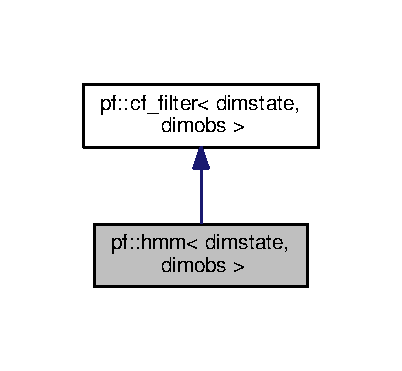
\includegraphics[width=193pt]{classpf_1_1hmm__inherit__graph}
\end{center}
\end{figure}


Collaboration diagram for pf\+:\+:hmm$<$ dimstate, dimobs $>$\+:
\nopagebreak
\begin{figure}[H]
\begin{center}
\leavevmode
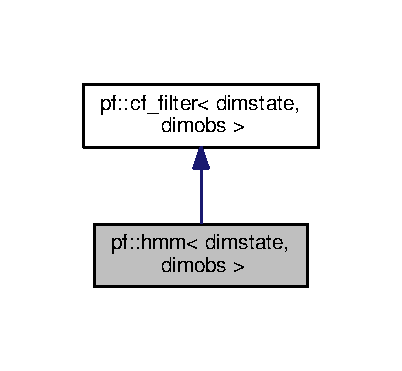
\includegraphics[width=193pt]{classpf_1_1hmm__coll__graph}
\end{center}
\end{figure}
\subsection*{Public Types}
\begin{DoxyCompactItemize}
\item 
using \hyperlink{classpf_1_1hmm_a62885209a039ac5483ccc4d07337f901}{ssv} = Eigen\+::\+Matrix$<$ double, dimstate, 1 $>$\hypertarget{classpf_1_1hmm_a62885209a039ac5483ccc4d07337f901}{}\label{classpf_1_1hmm_a62885209a039ac5483ccc4d07337f901}

\begin{DoxyCompactList}\small\item\em \char`\"{}state size vector\char`\"{} \end{DoxyCompactList}\item 
using \hyperlink{classpf_1_1hmm_a0c2ddb935318a9c320c9808e7820a9cb}{osv} = Eigen\+::\+Matrix$<$ double, dimobs, 1 $>$\hypertarget{classpf_1_1hmm_a0c2ddb935318a9c320c9808e7820a9cb}{}\label{classpf_1_1hmm_a0c2ddb935318a9c320c9808e7820a9cb}

\begin{DoxyCompactList}\small\item\em \char`\"{}observation size vector\char`\"{} \end{DoxyCompactList}\item 
using \hyperlink{classpf_1_1hmm_aa6e481316a30758d0eae33dbc8b5e8b5}{ss\+Mat} = Eigen\+::\+Matrix$<$ double, dimstate, dimstate $>$\hypertarget{classpf_1_1hmm_aa6e481316a30758d0eae33dbc8b5e8b5}{}\label{classpf_1_1hmm_aa6e481316a30758d0eae33dbc8b5e8b5}

\begin{DoxyCompactList}\small\item\em \char`\"{}state size matrix\char`\"{} \end{DoxyCompactList}\end{DoxyCompactItemize}
\subsection*{Public Member Functions}
\begin{DoxyCompactItemize}
\item 
\hyperlink{classpf_1_1hmm_a17382f741bd3f7c3729bcabdb2764dcf}{hmm} (const \hyperlink{classpf_1_1cf__filter_a448f675e130ac4b340e2c3e545673d0d}{ssv} \&init\+State\+Distr, const \hyperlink{classpf_1_1hmm_aa6e481316a30758d0eae33dbc8b5e8b5}{ss\+Mat} \&trans\+Mat)
\begin{DoxyCompactList}\small\item\em Constructor. \end{DoxyCompactList}\item 
double \hyperlink{classpf_1_1hmm_a61628b522c0eb71e9cf68d6956893169}{get\+Log\+Cond\+Like} () const 
\begin{DoxyCompactList}\small\item\em Get the latest conditional likelihood. \end{DoxyCompactList}\item 
\hyperlink{classpf_1_1cf__filter_a448f675e130ac4b340e2c3e545673d0d}{ssv} \hyperlink{classpf_1_1hmm_aa49d415c2bf87b87b1b95ab83f4dc830}{get\+Filter\+Vec} () const 
\begin{DoxyCompactList}\small\item\em Get the current filter vector. \end{DoxyCompactList}\item 
void \hyperlink{classpf_1_1hmm_a007ccf4612b26ca13b8bec2535171859}{update} (const \hyperlink{classpf_1_1cf__filter_ace17376128bb73ee73ff1b5c4972b317}{osv} \&yt, const \hyperlink{classpf_1_1cf__filter_a448f675e130ac4b340e2c3e545673d0d}{ssv} \&cond\+Dens\+Vec)
\begin{DoxyCompactList}\small\item\em Perform a H\+MM filter update. \end{DoxyCompactList}\end{DoxyCompactItemize}
\subsection*{Private Attributes}
\begin{DoxyCompactItemize}
\item 
\hyperlink{classpf_1_1cf__filter_a448f675e130ac4b340e2c3e545673d0d}{ssv} \hyperlink{classpf_1_1hmm_af3e6a0ffd2a9073d07b1b4bba3437d6a}{m\+\_\+filt\+Vec}\hypertarget{classpf_1_1hmm_af3e6a0ffd2a9073d07b1b4bba3437d6a}{}\label{classpf_1_1hmm_af3e6a0ffd2a9073d07b1b4bba3437d6a}

\begin{DoxyCompactList}\small\item\em filter vector \end{DoxyCompactList}\item 
\hyperlink{classpf_1_1hmm_aa6e481316a30758d0eae33dbc8b5e8b5}{ss\+Mat} \hyperlink{classpf_1_1hmm_a7f8d3cc9e3464a32e3e989a844a09012}{m\+\_\+trans\+Mat\+Transpose}\hypertarget{classpf_1_1hmm_a7f8d3cc9e3464a32e3e989a844a09012}{}\label{classpf_1_1hmm_a7f8d3cc9e3464a32e3e989a844a09012}

\begin{DoxyCompactList}\small\item\em transition matrix \end{DoxyCompactList}\item 
double \hyperlink{classpf_1_1hmm_adb7281566c6e48ec1691a0b8b13b385a}{m\+\_\+last\+Cond\+Like}\hypertarget{classpf_1_1hmm_adb7281566c6e48ec1691a0b8b13b385a}{}\label{classpf_1_1hmm_adb7281566c6e48ec1691a0b8b13b385a}

\begin{DoxyCompactList}\small\item\em last conditional likelihood \end{DoxyCompactList}\item 
bool \hyperlink{classpf_1_1hmm_a2923531a766aa61f30078fba49caf6b7}{m\+\_\+fresh}\hypertarget{classpf_1_1hmm_a2923531a766aa61f30078fba49caf6b7}{}\label{classpf_1_1hmm_a2923531a766aa61f30078fba49caf6b7}

\begin{DoxyCompactList}\small\item\em has data been observed? \end{DoxyCompactList}\end{DoxyCompactItemize}


\subsection{Constructor \& Destructor Documentation}
\index{pf\+::hmm@{pf\+::hmm}!hmm@{hmm}}
\index{hmm@{hmm}!pf\+::hmm@{pf\+::hmm}}
\subsubsection[{\texorpdfstring{hmm(const ssv \&init\+State\+Distr, const ss\+Mat \&trans\+Mat)}{hmm(const ssv &initStateDistr, const ssMat &transMat)}}]{\setlength{\rightskip}{0pt plus 5cm}template$<$size\+\_\+t dimstate, size\+\_\+t dimobs$>$ {\bf pf\+::hmm}$<$ dimstate, dimobs $>$\+::{\bf hmm} (
\begin{DoxyParamCaption}
\item[{const {\bf ssv} \&}]{init\+State\+Distr, }
\item[{const {\bf ss\+Mat} \&}]{trans\+Mat}
\end{DoxyParamCaption}
)}\hypertarget{classpf_1_1hmm_a17382f741bd3f7c3729bcabdb2764dcf}{}\label{classpf_1_1hmm_a17382f741bd3f7c3729bcabdb2764dcf}


Constructor. 


\begin{DoxyParams}{Parameters}
{\em init\+State\+Distr} & first time state prior distribution. \\
\hline
{\em trans\+Mat} & time homogeneous transition matrix. \\
\hline
\end{DoxyParams}


\subsection{Member Function Documentation}
\index{pf\+::hmm@{pf\+::hmm}!get\+Filter\+Vec@{get\+Filter\+Vec}}
\index{get\+Filter\+Vec@{get\+Filter\+Vec}!pf\+::hmm@{pf\+::hmm}}
\subsubsection[{\texorpdfstring{get\+Filter\+Vec() const }{getFilterVec() const }}]{\setlength{\rightskip}{0pt plus 5cm}template$<$size\+\_\+t dimstate, size\+\_\+t dimobs$>$ {\bf ssv} {\bf pf\+::hmm}$<$ dimstate, dimobs $>$\+::get\+Filter\+Vec (
\begin{DoxyParamCaption}
{}
\end{DoxyParamCaption}
) const}\hypertarget{classpf_1_1hmm_aa49d415c2bf87b87b1b95ab83f4dc830}{}\label{classpf_1_1hmm_aa49d415c2bf87b87b1b95ab83f4dc830}


Get the current filter vector. 

get the current filter vector. \begin{DoxyReturn}{Returns}
a probability vector p(x\+\_\+t $\vert$ y\+\_\+\{1\+:t\}) 
\end{DoxyReturn}
\index{pf\+::hmm@{pf\+::hmm}!get\+Log\+Cond\+Like@{get\+Log\+Cond\+Like}}
\index{get\+Log\+Cond\+Like@{get\+Log\+Cond\+Like}!pf\+::hmm@{pf\+::hmm}}
\subsubsection[{\texorpdfstring{get\+Log\+Cond\+Like() const }{getLogCondLike() const }}]{\setlength{\rightskip}{0pt plus 5cm}template$<$size\+\_\+t dimstate, size\+\_\+t dimobs$>$ double {\bf pf\+::hmm}$<$ dimstate, dimobs $>$\+::get\+Log\+Cond\+Like (
\begin{DoxyParamCaption}
{}
\end{DoxyParamCaption}
) const\hspace{0.3cm}{\ttfamily [virtual]}}\hypertarget{classpf_1_1hmm_a61628b522c0eb71e9cf68d6956893169}{}\label{classpf_1_1hmm_a61628b522c0eb71e9cf68d6956893169}


Get the latest conditional likelihood. 

\begin{DoxyReturn}{Returns}
the latest conditional likelihood. 
\end{DoxyReturn}


Implements \hyperlink{classpf_1_1cf__filter_ad9bce9703f26f5371973ceef5e253c4b}{pf\+::cf\+\_\+filter$<$ dimstate, dimobs $>$}.

\index{pf\+::hmm@{pf\+::hmm}!update@{update}}
\index{update@{update}!pf\+::hmm@{pf\+::hmm}}
\subsubsection[{\texorpdfstring{update(const osv \&yt, const ssv \&cond\+Dens\+Vec)}{update(const osv &yt, const ssv &condDensVec)}}]{\setlength{\rightskip}{0pt plus 5cm}template$<$size\+\_\+t dimstate, size\+\_\+t dimobs$>$ void {\bf pf\+::hmm}$<$ dimstate, dimobs $>$\+::update (
\begin{DoxyParamCaption}
\item[{const {\bf osv} \&}]{yt, }
\item[{const {\bf ssv} \&}]{cond\+Dens\+Vec}
\end{DoxyParamCaption}
)}\hypertarget{classpf_1_1hmm_a007ccf4612b26ca13b8bec2535171859}{}\label{classpf_1_1hmm_a007ccf4612b26ca13b8bec2535171859}


Perform a H\+MM filter update. 

Perform a H\+MM filter update. 
\begin{DoxyParams}{Parameters}
{\em yt} & the current datum. \\
\hline
{\em cond\+Dens\+Vec} & the vector (in x\+\_\+t) of p(y\+\_\+t$\vert$x\+\_\+t) \\
\hline
\end{DoxyParams}


The documentation for this class was generated from the following file\+:\begin{DoxyCompactItemize}
\item 
include/\hyperlink{cf__filters_8h}{cf\+\_\+filters.\+h}\end{DoxyCompactItemize}

\hypertarget{classpf_1_1k__gen}{}\section{pf\+:\+:k\+\_\+gen$<$ N $>$ Class Template Reference}
\label{classpf_1_1k__gen}\index{pf\+::k\+\_\+gen$<$ N $>$@{pf\+::k\+\_\+gen$<$ N $>$}}


A class that performs sampling with replacement (useful for the index sampler in an \hyperlink{classpf_1_1APF}{A\+PF})  




{\ttfamily \#include $<$rv\+\_\+samp.\+h$>$}



Inheritance diagram for pf\+:\+:k\+\_\+gen$<$ N $>$\+:\nopagebreak
\begin{figure}[H]
\begin{center}
\leavevmode
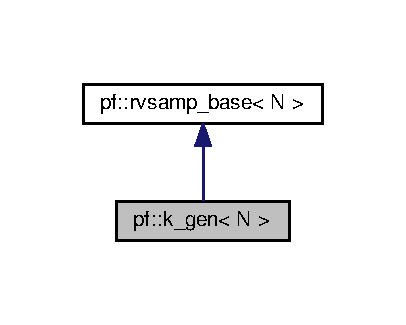
\includegraphics[width=195pt]{classpf_1_1k__gen__inherit__graph}
\end{center}
\end{figure}


Collaboration diagram for pf\+:\+:k\+\_\+gen$<$ N $>$\+:\nopagebreak
\begin{figure}[H]
\begin{center}
\leavevmode
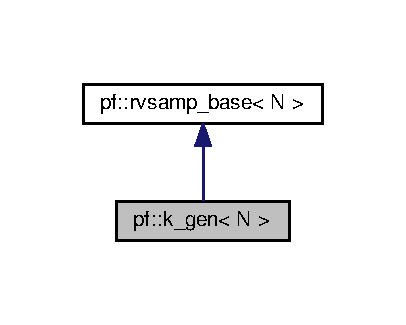
\includegraphics[width=195pt]{classpf_1_1k__gen__coll__graph}
\end{center}
\end{figure}
\subsection*{Public Member Functions}
\begin{DoxyCompactItemize}
\item 
\hyperlink{classpf_1_1k__gen_a484ba2a5755d8fa66ed20dd9e153f8f2}{k\+\_\+gen} ()\hypertarget{classpf_1_1k__gen_a484ba2a5755d8fa66ed20dd9e153f8f2}{}\label{classpf_1_1k__gen_a484ba2a5755d8fa66ed20dd9e153f8f2}

\begin{DoxyCompactList}\small\item\em default constructor. only one available. \end{DoxyCompactList}\item 
std\+::array$<$ unsigned int, N $>$ \hyperlink{classpf_1_1k__gen_a8eb63d23aaf6b4bd3a4faa10add1b790}{sample} (const std\+::array$<$ double, N $>$ \&log\+Wts)
\begin{DoxyCompactList}\small\item\em sample N times from (0,1,...N-\/1) \end{DoxyCompactList}\end{DoxyCompactItemize}
\subsection*{Additional Inherited Members}


\subsection{Detailed Description}
\subsubsection*{template$<$size\+\_\+t N$>$\\*
class pf\+::k\+\_\+gen$<$ N $>$}

A class that performs sampling with replacement (useful for the index sampler in an \hyperlink{classpf_1_1APF}{A\+PF}) 

\begin{DoxyAuthor}{Author}
taylor 
\end{DoxyAuthor}


\subsection{Member Function Documentation}
\index{pf\+::k\+\_\+gen@{pf\+::k\+\_\+gen}!sample@{sample}}
\index{sample@{sample}!pf\+::k\+\_\+gen@{pf\+::k\+\_\+gen}}
\subsubsection[{\texorpdfstring{sample(const std\+::array$<$ double, N $>$ \&log\+Wts)}{sample(const std::array< double, N > &logWts)}}]{\setlength{\rightskip}{0pt plus 5cm}template$<$size\+\_\+t N$>$ std\+::array$<$ unsigned int, N $>$ {\bf pf\+::k\+\_\+gen}$<$ N $>$\+::sample (
\begin{DoxyParamCaption}
\item[{const std\+::array$<$ double, N $>$ \&}]{log\+Wts}
\end{DoxyParamCaption}
)}\hypertarget{classpf_1_1k__gen_a8eb63d23aaf6b4bd3a4faa10add1b790}{}\label{classpf_1_1k__gen_a8eb63d23aaf6b4bd3a4faa10add1b790}


sample N times from (0,1,...N-\/1) 


\begin{DoxyParams}{Parameters}
{\em log\+Wts} & possibly unnormalized type std\+::array$<$double, N$>$ \\
\hline
\end{DoxyParams}
\begin{DoxyReturn}{Returns}
the integers in a std\+::array$<$unsigned int, N$>$ 
\end{DoxyReturn}


The documentation for this class was generated from the following file\+:\begin{DoxyCompactItemize}
\item 
include/\hyperlink{rv__samp_8h}{rv\+\_\+samp.\+h}\end{DoxyCompactItemize}

\hypertarget{classpf_1_1kalman}{}\section{pf\+:\+:kalman$<$ dimstate, dimobs, diminput $>$ Class Template Reference}
\label{classpf_1_1kalman}\index{pf\+::kalman$<$ dimstate, dimobs, diminput $>$@{pf\+::kalman$<$ dimstate, dimobs, diminput $>$}}


A class template for Kalman filtering.  




{\ttfamily \#include $<$cf\+\_\+filters.\+h$>$}

\subsection*{Private Types}
\begin{DoxyCompactItemize}
\item 
using \hyperlink{classpf_1_1kalman_a5b389e6a5e41f4ad81d4ba115d9aa823}{ssv} = Eigen\+::\+Matrix$<$ double, dimstate, 1 $>$
\item 
using \hyperlink{classpf_1_1kalman_a0568355548ed0e2cae065b489b2428c1}{osv} = Eigen\+::\+Matrix$<$ double, dimobs, 1 $>$
\item 
using \hyperlink{classpf_1_1kalman_a6cbcd532087d0b69bcf1825d8d4ac25a}{isv} = Eigen\+::\+Matrix$<$ double, diminput, 1 $>$
\item 
using \hyperlink{classpf_1_1kalman_aff9ecb9b57dfc3f115a372a765781561}{ss\+Mat} = Eigen\+::\+Matrix$<$ double, dimstate, dimstate $>$
\item 
using \hyperlink{classpf_1_1kalman_a41a83764417fa43c3eb0898676791efa}{os\+Mat} = Eigen\+::\+Matrix$<$ double, dimobs, dimobs $>$
\item 
using \hyperlink{classpf_1_1kalman_afc940e82542b4dcce4a0834297d98781}{si\+Mat} = Eigen\+::\+Matrix$<$ double, dimstate, diminput $>$
\item 
using \hyperlink{classpf_1_1kalman_a420f98a9c405f6b05987adafa82e8b52}{os\+Mat} = Eigen\+::\+Matrix$<$ double, dimobs, dimstate $>$
\item 
using \hyperlink{classpf_1_1kalman_a1bef1b09ec25689b765bb57bf1bbbfd6}{io\+Mat} = Eigen\+::\+Matrix$<$ double, dimobs, diminput $>$
\end{DoxyCompactItemize}
\subsection*{Private Member Functions}
\begin{DoxyCompactItemize}
\item 
\hyperlink{classpf_1_1kalman_a14f7c39ebc7d06f703a9cb08ae7c1c50}{kalman} (const \hyperlink{classpf_1_1kalman_a5b389e6a5e41f4ad81d4ba115d9aa823}{ssv} \&init\+State\+Mean, const Mat \&init\+State\+Var) double get\+Log\+Cond\+Like() const 
\begin{DoxyCompactList}\small\item\em Non-\/default constructor. \end{DoxyCompactList}\item 
\hyperlink{classpf_1_1kalman_a5b389e6a5e41f4ad81d4ba115d9aa823}{ssv} \hyperlink{classpf_1_1kalman_aeede6326045fa762468cdb9f24d4c22a}{get\+Filt\+Mean} () const 
\begin{DoxyCompactList}\small\item\em Get the current filter mean. \end{DoxyCompactList}\item 
Mat \hyperlink{classpf_1_1kalman_a1c969734ffe8ea15dcfdc440cc2e1181}{get\+Filt\+Var} () const 
\begin{DoxyCompactList}\small\item\em Get the current filter variance-\/covariance matrix. \end{DoxyCompactList}\item 
void \hyperlink{classpf_1_1kalman_a081bf6466cc9d19e72ef50cf1ca4bc00}{update} (const \hyperlink{classpf_1_1kalman_a0568355548ed0e2cae065b489b2428c1}{osv} \&yt, const \hyperlink{classpf_1_1kalman_aff9ecb9b57dfc3f115a372a765781561}{ss\+Mat} \&state\+Trans, const \hyperlink{classpf_1_1kalman_aff9ecb9b57dfc3f115a372a765781561}{ss\+Mat} \&chol\+State\+Var, const \hyperlink{classpf_1_1kalman_afc940e82542b4dcce4a0834297d98781}{si\+Mat} \&state\+Inpt\+Affector, const \hyperlink{classpf_1_1kalman_a6cbcd532087d0b69bcf1825d8d4ac25a}{isv} \&input\+Data, const \hyperlink{classpf_1_1kalman_a41a83764417fa43c3eb0898676791efa}{os\+Mat} \&obs\+Mat, const \hyperlink{classpf_1_1kalman_a1bef1b09ec25689b765bb57bf1bbbfd6}{io\+Mat} \&obs\+Inpt\+Affector, const \hyperlink{classpf_1_1kalman_a41a83764417fa43c3eb0898676791efa}{os\+Mat} \&chol\+Obs\+Var)
\begin{DoxyCompactList}\small\item\em Perform a Kalman filter predict-\/and-\/update. \end{DoxyCompactList}\item 
void \hyperlink{classpf_1_1kalman_ada09b42d4d99ea42b89e7d4a192d59a1}{update\+Prior} (const \hyperlink{classpf_1_1kalman_aff9ecb9b57dfc3f115a372a765781561}{ss\+Mat} \&state\+Trans\+Mat, const \hyperlink{classpf_1_1kalman_aff9ecb9b57dfc3f115a372a765781561}{ss\+Mat} \&chol\+State\+Var, const \hyperlink{classpf_1_1kalman_afc940e82542b4dcce4a0834297d98781}{si\+Mat} \&state\+Inpt\+Affector, const \hyperlink{classpf_1_1kalman_a6cbcd532087d0b69bcf1825d8d4ac25a}{isv} \&input\+Data)
\begin{DoxyCompactList}\small\item\em Predicts the next state. \end{DoxyCompactList}\item 
void \hyperlink{classpf_1_1kalman_a75a2c684bb44815258fb91f1b66ed9c0}{update\+Posterior} (const \hyperlink{classpf_1_1kalman_a0568355548ed0e2cae065b489b2428c1}{osv} \&yt, const \hyperlink{classpf_1_1kalman_a41a83764417fa43c3eb0898676791efa}{os\+Mat} \&obs\+Mat, const oi\+Mat \&obs\+Inpt\+Affector, const \hyperlink{classpf_1_1kalman_a6cbcd532087d0b69bcf1825d8d4ac25a}{isv} \&input\+Data, const \hyperlink{classpf_1_1kalman_a41a83764417fa43c3eb0898676791efa}{os\+Mat} \&chol\+Obs\+Var)
\begin{DoxyCompactList}\small\item\em Turns prediction into new filtering distribution. \end{DoxyCompactList}\end{DoxyCompactItemize}
\subsection*{Private Attributes}
\begin{DoxyCompactItemize}
\item 
\hyperlink{classpf_1_1kalman_a5b389e6a5e41f4ad81d4ba115d9aa823}{ssv} \hyperlink{classpf_1_1kalman_a3bdb45825b162f620e3ce10c5d2505fc}{m\+\_\+pred\+Mean}\hypertarget{classpf_1_1kalman_a3bdb45825b162f620e3ce10c5d2505fc}{}\label{classpf_1_1kalman_a3bdb45825b162f620e3ce10c5d2505fc}

\begin{DoxyCompactList}\small\item\em predictive state mean \end{DoxyCompactList}\item 
\hyperlink{classpf_1_1kalman_a5b389e6a5e41f4ad81d4ba115d9aa823}{ssv} \hyperlink{classpf_1_1kalman_adda10a5a5cbe413a247f9125598fa95c}{m\+\_\+filt\+Mean}\hypertarget{classpf_1_1kalman_adda10a5a5cbe413a247f9125598fa95c}{}\label{classpf_1_1kalman_adda10a5a5cbe413a247f9125598fa95c}

\begin{DoxyCompactList}\small\item\em filter mean \end{DoxyCompactList}\item 
\hyperlink{classpf_1_1kalman_aff9ecb9b57dfc3f115a372a765781561}{ss\+Mat} \hyperlink{classpf_1_1kalman_aa7ff59d149e1946ea7efe9c0df7b5cea}{m\+\_\+pred\+Var}\hypertarget{classpf_1_1kalman_aa7ff59d149e1946ea7efe9c0df7b5cea}{}\label{classpf_1_1kalman_aa7ff59d149e1946ea7efe9c0df7b5cea}

\begin{DoxyCompactList}\small\item\em predictive var matrix \end{DoxyCompactList}\item 
\hyperlink{classpf_1_1kalman_aff9ecb9b57dfc3f115a372a765781561}{ss\+Mat} \hyperlink{classpf_1_1kalman_a7757b7c2ddf87bb063774ebce5210685}{m\+\_\+filt\+Var}\hypertarget{classpf_1_1kalman_a7757b7c2ddf87bb063774ebce5210685}{}\label{classpf_1_1kalman_a7757b7c2ddf87bb063774ebce5210685}

\begin{DoxyCompactList}\small\item\em filter var matrix \end{DoxyCompactList}\item 
double \hyperlink{classpf_1_1kalman_ac8cfb255218900a3234be942b5ca903f}{m\+\_\+last\+Log\+Cond\+Like}\hypertarget{classpf_1_1kalman_ac8cfb255218900a3234be942b5ca903f}{}\label{classpf_1_1kalman_ac8cfb255218900a3234be942b5ca903f}

\begin{DoxyCompactList}\small\item\em latest log conditional likelihood \end{DoxyCompactList}\item 
bool \hyperlink{classpf_1_1kalman_a0eee8bb578016b1e9600ffd2c9f23aa9}{m\+\_\+fresh}\hypertarget{classpf_1_1kalman_a0eee8bb578016b1e9600ffd2c9f23aa9}{}\label{classpf_1_1kalman_a0eee8bb578016b1e9600ffd2c9f23aa9}

\begin{DoxyCompactList}\small\item\em has data been observed? \end{DoxyCompactList}\end{DoxyCompactItemize}


\subsection{Detailed Description}
\subsubsection*{template$<$size\+\_\+t dimstate, size\+\_\+t dimobs, size\+\_\+t diminput$>$\\*
class pf\+::kalman$<$ dimstate, dimobs, diminput $>$}

A class template for Kalman filtering. 

\begin{DoxyAuthor}{Author}
taylor 
\end{DoxyAuthor}


\subsection{Member Typedef Documentation}
\index{pf\+::kalman@{pf\+::kalman}!io\+Mat@{io\+Mat}}
\index{io\+Mat@{io\+Mat}!pf\+::kalman@{pf\+::kalman}}
\subsubsection[{\texorpdfstring{io\+Mat}{ioMat}}]{\setlength{\rightskip}{0pt plus 5cm}template$<$size\+\_\+t dimstate, size\+\_\+t dimobs, size\+\_\+t diminput$>$ using {\bf pf\+::kalman}$<$ dimstate, dimobs, diminput $>$\+::{\bf io\+Mat} =  Eigen\+::\+Matrix$<$double,dimobs,diminput$>$\hspace{0.3cm}{\ttfamily [private]}}\hypertarget{classpf_1_1kalman_a1bef1b09ec25689b765bb57bf1bbbfd6}{}\label{classpf_1_1kalman_a1bef1b09ec25689b765bb57bf1bbbfd6}
\char`\"{}input dim by observation dimension matrix\char`\"{} \index{pf\+::kalman@{pf\+::kalman}!isv@{isv}}
\index{isv@{isv}!pf\+::kalman@{pf\+::kalman}}
\subsubsection[{\texorpdfstring{isv}{isv}}]{\setlength{\rightskip}{0pt plus 5cm}template$<$size\+\_\+t dimstate, size\+\_\+t dimobs, size\+\_\+t diminput$>$ using {\bf pf\+::kalman}$<$ dimstate, dimobs, diminput $>$\+::{\bf isv} =  Eigen\+::\+Matrix$<$double,diminput,1$>$\hspace{0.3cm}{\ttfamily [private]}}\hypertarget{classpf_1_1kalman_a6cbcd532087d0b69bcf1825d8d4ac25a}{}\label{classpf_1_1kalman_a6cbcd532087d0b69bcf1825d8d4ac25a}
\char`\"{}input size vector\char`\"{} type alias for linear algebra stuff \index{pf\+::kalman@{pf\+::kalman}!os\+Mat@{os\+Mat}}
\index{os\+Mat@{os\+Mat}!pf\+::kalman@{pf\+::kalman}}
\subsubsection[{\texorpdfstring{os\+Mat}{osMat}}]{\setlength{\rightskip}{0pt plus 5cm}template$<$size\+\_\+t dimstate, size\+\_\+t dimobs, size\+\_\+t diminput$>$ using {\bf pf\+::kalman}$<$ dimstate, dimobs, diminput $>$\+::{\bf os\+Mat} =  Eigen\+::\+Matrix$<$double,dimobs,dimobs$>$\hspace{0.3cm}{\ttfamily [private]}}\hypertarget{classpf_1_1kalman_a41a83764417fa43c3eb0898676791efa}{}\label{classpf_1_1kalman_a41a83764417fa43c3eb0898676791efa}
\char`\"{}observation size matrix\char`\"{} type alias for linear algebra stuff \index{pf\+::kalman@{pf\+::kalman}!os\+Mat@{os\+Mat}}
\index{os\+Mat@{os\+Mat}!pf\+::kalman@{pf\+::kalman}}
\subsubsection[{\texorpdfstring{os\+Mat}{osMat}}]{\setlength{\rightskip}{0pt plus 5cm}template$<$size\+\_\+t dimstate, size\+\_\+t dimobs, size\+\_\+t diminput$>$ using {\bf pf\+::kalman}$<$ dimstate, dimobs, diminput $>$\+::{\bf os\+Mat} =  Eigen\+::\+Matrix$<$double,dimobs,dimstate$>$\hspace{0.3cm}{\ttfamily [private]}}\hypertarget{classpf_1_1kalman_a420f98a9c405f6b05987adafa82e8b52}{}\label{classpf_1_1kalman_a420f98a9c405f6b05987adafa82e8b52}
\char`\"{}observation dim by state dimension matrix\char`\"{} \index{pf\+::kalman@{pf\+::kalman}!osv@{osv}}
\index{osv@{osv}!pf\+::kalman@{pf\+::kalman}}
\subsubsection[{\texorpdfstring{osv}{osv}}]{\setlength{\rightskip}{0pt plus 5cm}template$<$size\+\_\+t dimstate, size\+\_\+t dimobs, size\+\_\+t diminput$>$ using {\bf pf\+::kalman}$<$ dimstate, dimobs, diminput $>$\+::{\bf osv} =  Eigen\+::\+Matrix$<$double,dimobs,1$>$\hspace{0.3cm}{\ttfamily [private]}}\hypertarget{classpf_1_1kalman_a0568355548ed0e2cae065b489b2428c1}{}\label{classpf_1_1kalman_a0568355548ed0e2cae065b489b2428c1}
\char`\"{}observation size vector\char`\"{} type alias for linear algebra stuff \index{pf\+::kalman@{pf\+::kalman}!si\+Mat@{si\+Mat}}
\index{si\+Mat@{si\+Mat}!pf\+::kalman@{pf\+::kalman}}
\subsubsection[{\texorpdfstring{si\+Mat}{siMat}}]{\setlength{\rightskip}{0pt plus 5cm}template$<$size\+\_\+t dimstate, size\+\_\+t dimobs, size\+\_\+t diminput$>$ using {\bf pf\+::kalman}$<$ dimstate, dimobs, diminput $>$\+::{\bf si\+Mat} =  Eigen\+::\+Matrix$<$double,dimstate,diminput$>$\hspace{0.3cm}{\ttfamily [private]}}\hypertarget{classpf_1_1kalman_afc940e82542b4dcce4a0834297d98781}{}\label{classpf_1_1kalman_afc940e82542b4dcce4a0834297d98781}
\char`\"{}state dim by input dimension matrix\char`\"{} \index{pf\+::kalman@{pf\+::kalman}!ss\+Mat@{ss\+Mat}}
\index{ss\+Mat@{ss\+Mat}!pf\+::kalman@{pf\+::kalman}}
\subsubsection[{\texorpdfstring{ss\+Mat}{ssMat}}]{\setlength{\rightskip}{0pt plus 5cm}template$<$size\+\_\+t dimstate, size\+\_\+t dimobs, size\+\_\+t diminput$>$ using {\bf pf\+::kalman}$<$ dimstate, dimobs, diminput $>$\+::{\bf ss\+Mat} =  Eigen\+::\+Matrix$<$double,dimstate,dimstate$>$\hspace{0.3cm}{\ttfamily [private]}}\hypertarget{classpf_1_1kalman_aff9ecb9b57dfc3f115a372a765781561}{}\label{classpf_1_1kalman_aff9ecb9b57dfc3f115a372a765781561}
\char`\"{}state size matrix\char`\"{} type alias for linear algebra stuff \index{pf\+::kalman@{pf\+::kalman}!ssv@{ssv}}
\index{ssv@{ssv}!pf\+::kalman@{pf\+::kalman}}
\subsubsection[{\texorpdfstring{ssv}{ssv}}]{\setlength{\rightskip}{0pt plus 5cm}template$<$size\+\_\+t dimstate, size\+\_\+t dimobs, size\+\_\+t diminput$>$ using {\bf pf\+::kalman}$<$ dimstate, dimobs, diminput $>$\+::{\bf ssv} =  Eigen\+::\+Matrix$<$double,dimstate,1$>$\hspace{0.3cm}{\ttfamily [private]}}\hypertarget{classpf_1_1kalman_a5b389e6a5e41f4ad81d4ba115d9aa823}{}\label{classpf_1_1kalman_a5b389e6a5e41f4ad81d4ba115d9aa823}
\char`\"{}state size vector\char`\"{} type alias for linear algebra stuff 

\subsection{Constructor \& Destructor Documentation}
\index{pf\+::kalman@{pf\+::kalman}!kalman@{kalman}}
\index{kalman@{kalman}!pf\+::kalman@{pf\+::kalman}}
\subsubsection[{\texorpdfstring{kalman(const ssv \&init\+State\+Mean, const Mat \&init\+State\+Var) double get\+Log\+Cond\+Like() const }{kalman(const ssv &initStateMean, const Mat &initStateVar) double getLogCondLike() const }}]{\setlength{\rightskip}{0pt plus 5cm}template$<$size\+\_\+t dimstate, size\+\_\+t dimobs, size\+\_\+t diminput$>$ {\bf pf\+::kalman}$<$ dimstate, dimobs, diminput $>$\+::{\bf kalman} (
\begin{DoxyParamCaption}
\item[{const {\bf ssv} \&}]{init\+State\+Mean, }
\item[{const Mat \&}]{init\+State\+Var}
\end{DoxyParamCaption}
) const\hspace{0.3cm}{\ttfamily [private]}}\hypertarget{classpf_1_1kalman_a14f7c39ebc7d06f703a9cb08ae7c1c50}{}\label{classpf_1_1kalman_a14f7c39ebc7d06f703a9cb08ae7c1c50}


Non-\/default constructor. 

returns the log of the latest conditional likelihood. \begin{DoxyReturn}{Returns}
log p(y\+\_\+t $\vert$ y\+\_\+\{1\+:t-\/1\}) or log p(y\+\_\+1) 
\end{DoxyReturn}


\subsection{Member Function Documentation}
\index{pf\+::kalman@{pf\+::kalman}!get\+Filt\+Mean@{get\+Filt\+Mean}}
\index{get\+Filt\+Mean@{get\+Filt\+Mean}!pf\+::kalman@{pf\+::kalman}}
\subsubsection[{\texorpdfstring{get\+Filt\+Mean() const }{getFiltMean() const }}]{\setlength{\rightskip}{0pt plus 5cm}template$<$size\+\_\+t dimstate, size\+\_\+t dimobs, size\+\_\+t diminput$>$ auto {\bf pf\+::kalman}$<$ dimstate, dimobs, diminput $>$\+::get\+Filt\+Mean (
\begin{DoxyParamCaption}
{}
\end{DoxyParamCaption}
) const\hspace{0.3cm}{\ttfamily [private]}}\hypertarget{classpf_1_1kalman_aeede6326045fa762468cdb9f24d4c22a}{}\label{classpf_1_1kalman_aeede6326045fa762468cdb9f24d4c22a}


Get the current filter mean. 

\begin{DoxyReturn}{Returns}
E\mbox{[}x\+\_\+t $\vert$ y\+\_\+\{1\+:t\}\mbox{]} 
\end{DoxyReturn}
\index{pf\+::kalman@{pf\+::kalman}!get\+Filt\+Var@{get\+Filt\+Var}}
\index{get\+Filt\+Var@{get\+Filt\+Var}!pf\+::kalman@{pf\+::kalman}}
\subsubsection[{\texorpdfstring{get\+Filt\+Var() const }{getFiltVar() const }}]{\setlength{\rightskip}{0pt plus 5cm}template$<$size\+\_\+t dimstate, size\+\_\+t dimobs, size\+\_\+t diminput$>$ auto {\bf pf\+::kalman}$<$ dimstate, dimobs, diminput $>$\+::get\+Filt\+Var (
\begin{DoxyParamCaption}
{}
\end{DoxyParamCaption}
) const\hspace{0.3cm}{\ttfamily [private]}}\hypertarget{classpf_1_1kalman_a1c969734ffe8ea15dcfdc440cc2e1181}{}\label{classpf_1_1kalman_a1c969734ffe8ea15dcfdc440cc2e1181}


Get the current filter variance-\/covariance matrix. 

\begin{DoxyReturn}{Returns}
V\mbox{[}x\+\_\+t $\vert$ y\+\_\+\{1\+:t\}\mbox{]} 
\end{DoxyReturn}
\index{pf\+::kalman@{pf\+::kalman}!update@{update}}
\index{update@{update}!pf\+::kalman@{pf\+::kalman}}
\subsubsection[{\texorpdfstring{update(const osv \&yt, const ss\+Mat \&state\+Trans, const ss\+Mat \&chol\+State\+Var, const si\+Mat \&state\+Inpt\+Affector, const isv \&input\+Data, const os\+Mat \&obs\+Mat, const io\+Mat \&obs\+Inpt\+Affector, const os\+Mat \&chol\+Obs\+Var)}{update(const osv &yt, const ssMat &stateTrans, const ssMat &cholStateVar, const siMat &stateInptAffector, const isv &inputData, const osMat &obsMat, const ioMat &obsInptAffector, const osMat &cholObsVar)}}]{\setlength{\rightskip}{0pt plus 5cm}template$<$size\+\_\+t dimstate, size\+\_\+t dimobs, size\+\_\+t diminput$>$ void {\bf pf\+::kalman}$<$ dimstate, dimobs, diminput $>$\+::update (
\begin{DoxyParamCaption}
\item[{const {\bf osv} \&}]{yt, }
\item[{const {\bf ss\+Mat} \&}]{state\+Trans, }
\item[{const {\bf ss\+Mat} \&}]{chol\+State\+Var, }
\item[{const {\bf si\+Mat} \&}]{state\+Inpt\+Affector, }
\item[{const {\bf isv} \&}]{input\+Data, }
\item[{const {\bf os\+Mat} \&}]{obs\+Mat, }
\item[{const {\bf io\+Mat} \&}]{obs\+Inpt\+Affector, }
\item[{const {\bf os\+Mat} \&}]{chol\+Obs\+Var}
\end{DoxyParamCaption}
)\hspace{0.3cm}{\ttfamily [private]}}\hypertarget{classpf_1_1kalman_a081bf6466cc9d19e72ef50cf1ca4bc00}{}\label{classpf_1_1kalman_a081bf6466cc9d19e72ef50cf1ca4bc00}


Perform a Kalman filter predict-\/and-\/update. 


\begin{DoxyParams}{Parameters}
{\em yt} & the new data point. \\
\hline
{\em state\+Trans} & the transition matrix of the state \\
\hline
{\em chol\+State\+Var} & the Cholesky Decomposition of the state noise covariance matrix. \\
\hline
{\em state\+Inpt\+Affector} & the matrix affecting how input data affects state transition. \\
\hline
{\em input\+Data} & exogenous input data \\
\hline
{\em obs\+Mat} & the observation/emission matrix of the observation\textquotesingle{}s conditional (on the state) distn. \\
\hline
{\em obs\+Inpt\+Affector} & the matrix affecting how input data affects the observational distribution. \\
\hline
{\em chol\+Obs\+Var} & the Cholesky Decomposition of the observatio noise covariance matrix. \\
\hline
\end{DoxyParams}
\index{pf\+::kalman@{pf\+::kalman}!update\+Posterior@{update\+Posterior}}
\index{update\+Posterior@{update\+Posterior}!pf\+::kalman@{pf\+::kalman}}
\subsubsection[{\texorpdfstring{update\+Posterior(const osv \&yt, const os\+Mat \&obs\+Mat, const oi\+Mat \&obs\+Inpt\+Affector, const isv \&input\+Data, const os\+Mat \&chol\+Obs\+Var)}{updatePosterior(const osv &yt, const osMat &obsMat, const oiMat &obsInptAffector, const isv &inputData, const osMat &cholObsVar)}}]{\setlength{\rightskip}{0pt plus 5cm}template$<$size\+\_\+t dimstate, size\+\_\+t dimobs, size\+\_\+t diminput$>$ void {\bf pf\+::kalman}$<$ dimstate, dimobs, diminput $>$\+::update\+Posterior (
\begin{DoxyParamCaption}
\item[{const {\bf osv} \&}]{yt, }
\item[{const {\bf os\+Mat} \&}]{obs\+Mat, }
\item[{const oi\+Mat \&}]{obs\+Inpt\+Affector, }
\item[{const {\bf isv} \&}]{input\+Data, }
\item[{const {\bf os\+Mat} \&}]{chol\+Obs\+Var}
\end{DoxyParamCaption}
)\hspace{0.3cm}{\ttfamily [private]}}\hypertarget{classpf_1_1kalman_a75a2c684bb44815258fb91f1b66ed9c0}{}\label{classpf_1_1kalman_a75a2c684bb44815258fb91f1b66ed9c0}


Turns prediction into new filtering distribution. 


\begin{DoxyParams}{Parameters}
{\em yt} & \\
\hline
{\em obs\+Mat} & \\
\hline
{\em obs\+Inpt\+Affector} & \\
\hline
{\em input\+Data} & \\
\hline
{\em chol\+Obs\+Var} & \\
\hline
\end{DoxyParams}
\index{pf\+::kalman@{pf\+::kalman}!update\+Prior@{update\+Prior}}
\index{update\+Prior@{update\+Prior}!pf\+::kalman@{pf\+::kalman}}
\subsubsection[{\texorpdfstring{update\+Prior(const ss\+Mat \&state\+Trans\+Mat, const ss\+Mat \&chol\+State\+Var, const si\+Mat \&state\+Inpt\+Affector, const isv \&input\+Data)}{updatePrior(const ssMat &stateTransMat, const ssMat &cholStateVar, const siMat &stateInptAffector, const isv &inputData)}}]{\setlength{\rightskip}{0pt plus 5cm}template$<$size\+\_\+t dimstate, size\+\_\+t dimobs, size\+\_\+t diminput$>$ void {\bf pf\+::kalman}$<$ dimstate, dimobs, diminput $>$\+::update\+Prior (
\begin{DoxyParamCaption}
\item[{const {\bf ss\+Mat} \&}]{state\+Trans\+Mat, }
\item[{const {\bf ss\+Mat} \&}]{chol\+State\+Var, }
\item[{const {\bf si\+Mat} \&}]{state\+Inpt\+Affector, }
\item[{const {\bf isv} \&}]{input\+Data}
\end{DoxyParamCaption}
)\hspace{0.3cm}{\ttfamily [private]}}\hypertarget{classpf_1_1kalman_ada09b42d4d99ea42b89e7d4a192d59a1}{}\label{classpf_1_1kalman_ada09b42d4d99ea42b89e7d4a192d59a1}


Predicts the next state. 

\begin{DoxyRefDesc}{Todo}
\item[\hyperlink{todo__todo000002}{Todo}]handle diagonal variance matrices, and ensure symmetricness in other ways \end{DoxyRefDesc}

\begin{DoxyParams}{Parameters}
{\em state\+Trans\+Mat} & \\
\hline
{\em chol\+State\+Var} & \\
\hline
{\em state\+Inpt\+Affector} & \\
\hline
{\em input\+Data} & \\
\hline
\end{DoxyParams}


The documentation for this class was generated from the following file\+:\begin{DoxyCompactItemize}
\item 
include/\hyperlink{cf__filters_8h}{cf\+\_\+filters.\+h}\end{DoxyCompactItemize}

\hypertarget{classpf_1_1mn__resampler}{}\section{pf\+:\+:mn\+\_\+resampler$<$ nparts, dimx $>$ Class Template Reference}
\label{classpf_1_1mn__resampler}\index{pf\+::mn\+\_\+resampler$<$ nparts, dimx $>$@{pf\+::mn\+\_\+resampler$<$ nparts, dimx $>$}}


Performs multinomial resampling.  




{\ttfamily \#include $<$resamplers.\+h$>$}



Inheritance diagram for pf\+:\+:mn\+\_\+resampler$<$ nparts, dimx $>$\+:\nopagebreak
\begin{figure}[H]
\begin{center}
\leavevmode
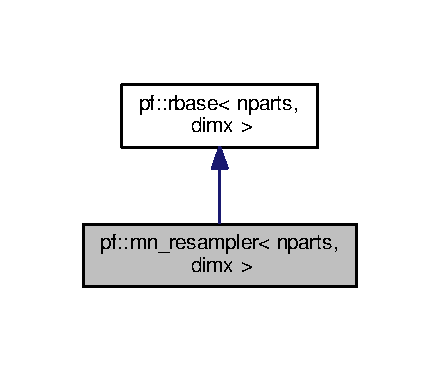
\includegraphics[width=211pt]{classpf_1_1mn__resampler__inherit__graph}
\end{center}
\end{figure}


Collaboration diagram for pf\+:\+:mn\+\_\+resampler$<$ nparts, dimx $>$\+:\nopagebreak
\begin{figure}[H]
\begin{center}
\leavevmode
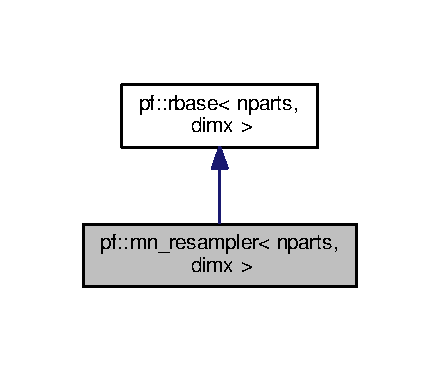
\includegraphics[width=211pt]{classpf_1_1mn__resampler__coll__graph}
\end{center}
\end{figure}
\subsection*{Public Types}
\begin{DoxyCompactItemize}
\item 
using \hyperlink{classpf_1_1mn__resampler_a88c55c4d05bf91b0a2e6c07d889e94bf}{ssv} = Eigen\+::\+Matrix$<$ double, dimx, 1 $>$
\item 
using \hyperlink{classpf_1_1mn__resampler_a42375cc080fb301e33d323c3ceb34f20}{array\+Vec} = std\+::array$<$ \hyperlink{classpf_1_1rbase_a47a4bdc0e3c08b72ce4f24a18d5b0e04}{ssv}, nparts $>$
\item 
using \hyperlink{classpf_1_1mn__resampler_a955686138dfb4b814c02eca3d1fc0fa9}{array\+Double} = std\+::array$<$ double, nparts $>$
\item 
using \hyperlink{classpf_1_1mn__resampler_a72e4f61199b83289d694323a05fdd1ef}{array\+Int} = std\+::array$<$ unsigned int, nparts $>$
\end{DoxyCompactItemize}
\subsection*{Public Member Functions}
\begin{DoxyCompactItemize}
\item 
\hyperlink{classpf_1_1mn__resampler_a085cc0be4c278d949b27e2eac17180d6}{mn\+\_\+resampler} ()\hypertarget{classpf_1_1mn__resampler_a085cc0be4c278d949b27e2eac17180d6}{}\label{classpf_1_1mn__resampler_a085cc0be4c278d949b27e2eac17180d6}

\begin{DoxyCompactList}\small\item\em Default constructor. Only option available. \end{DoxyCompactList}\item 
void \hyperlink{classpf_1_1mn__resampler_a9fe1aa27517fc0333f2fa82653a4d9fc}{resamp\+Log\+Wts} (\hyperlink{classpf_1_1rbase_a89951bb3872c1c6a0c3da0962a9aaa13}{array\+Vec} \&old\+Parts, \hyperlink{classpf_1_1rbase_a37b2d02d00f75d9550122b763cbb3fed}{array\+Double} \&old\+Log\+Un\+Norm\+Wts)
\begin{DoxyCompactList}\small\item\em resamples particles. \end{DoxyCompactList}\end{DoxyCompactItemize}
\subsection*{Private Attributes}
\begin{DoxyCompactItemize}
\item 
std\+::mt19937 \hyperlink{classpf_1_1mn__resampler_a463059a4eed72e18bc02034bfe4bb8f3}{m\+\_\+gen}\hypertarget{classpf_1_1mn__resampler_a463059a4eed72e18bc02034bfe4bb8f3}{}\label{classpf_1_1mn__resampler_a463059a4eed72e18bc02034bfe4bb8f3}

\begin{DoxyCompactList}\small\item\em prng \end{DoxyCompactList}\end{DoxyCompactItemize}


\subsection{Detailed Description}
\subsubsection*{template$<$size\+\_\+t nparts, size\+\_\+t dimx$>$\\*
class pf\+::mn\+\_\+resampler$<$ nparts, dimx $>$}

Performs multinomial resampling. 

\begin{DoxyAuthor}{Author}
taylor 
\end{DoxyAuthor}
\begin{DoxyDate}{Date}
15/04/18 
\end{DoxyDate}


\subsection{Member Typedef Documentation}
\index{pf\+::mn\+\_\+resampler@{pf\+::mn\+\_\+resampler}!array\+Double@{array\+Double}}
\index{array\+Double@{array\+Double}!pf\+::mn\+\_\+resampler@{pf\+::mn\+\_\+resampler}}
\subsubsection[{\texorpdfstring{array\+Double}{arrayDouble}}]{\setlength{\rightskip}{0pt plus 5cm}template$<$size\+\_\+t nparts, size\+\_\+t dimx$>$ using {\bf pf\+::mn\+\_\+resampler}$<$ nparts, dimx $>$\+::{\bf array\+Double} =  std\+::array$<$double,nparts$>$}\hypertarget{classpf_1_1mn__resampler_a955686138dfb4b814c02eca3d1fc0fa9}{}\label{classpf_1_1mn__resampler_a955686138dfb4b814c02eca3d1fc0fa9}
type alias for array of doubles \index{pf\+::mn\+\_\+resampler@{pf\+::mn\+\_\+resampler}!array\+Int@{array\+Int}}
\index{array\+Int@{array\+Int}!pf\+::mn\+\_\+resampler@{pf\+::mn\+\_\+resampler}}
\subsubsection[{\texorpdfstring{array\+Int}{arrayInt}}]{\setlength{\rightskip}{0pt plus 5cm}template$<$size\+\_\+t nparts, size\+\_\+t dimx$>$ using {\bf pf\+::mn\+\_\+resampler}$<$ nparts, dimx $>$\+::{\bf array\+Int} =  std\+::array$<$unsigned int,nparts$>$}\hypertarget{classpf_1_1mn__resampler_a72e4f61199b83289d694323a05fdd1ef}{}\label{classpf_1_1mn__resampler_a72e4f61199b83289d694323a05fdd1ef}
type alias for array of integers \index{pf\+::mn\+\_\+resampler@{pf\+::mn\+\_\+resampler}!array\+Vec@{array\+Vec}}
\index{array\+Vec@{array\+Vec}!pf\+::mn\+\_\+resampler@{pf\+::mn\+\_\+resampler}}
\subsubsection[{\texorpdfstring{array\+Vec}{arrayVec}}]{\setlength{\rightskip}{0pt plus 5cm}template$<$size\+\_\+t nparts, size\+\_\+t dimx$>$ using {\bf pf\+::mn\+\_\+resampler}$<$ nparts, dimx $>$\+::{\bf array\+Vec} =  std\+::array$<${\bf ssv}, nparts$>$}\hypertarget{classpf_1_1mn__resampler_a42375cc080fb301e33d323c3ceb34f20}{}\label{classpf_1_1mn__resampler_a42375cc080fb301e33d323c3ceb34f20}
type alias for linear algebra stuff \index{pf\+::mn\+\_\+resampler@{pf\+::mn\+\_\+resampler}!ssv@{ssv}}
\index{ssv@{ssv}!pf\+::mn\+\_\+resampler@{pf\+::mn\+\_\+resampler}}
\subsubsection[{\texorpdfstring{ssv}{ssv}}]{\setlength{\rightskip}{0pt plus 5cm}template$<$size\+\_\+t nparts, size\+\_\+t dimx$>$ using {\bf pf\+::mn\+\_\+resampler}$<$ nparts, dimx $>$\+::{\bf ssv} =  Eigen\+::\+Matrix$<$double,dimx,1$>$}\hypertarget{classpf_1_1mn__resampler_a88c55c4d05bf91b0a2e6c07d889e94bf}{}\label{classpf_1_1mn__resampler_a88c55c4d05bf91b0a2e6c07d889e94bf}
type alias for linear algebra stuff 

\subsection{Member Function Documentation}
\index{pf\+::mn\+\_\+resampler@{pf\+::mn\+\_\+resampler}!resamp\+Log\+Wts@{resamp\+Log\+Wts}}
\index{resamp\+Log\+Wts@{resamp\+Log\+Wts}!pf\+::mn\+\_\+resampler@{pf\+::mn\+\_\+resampler}}
\subsubsection[{\texorpdfstring{resamp\+Log\+Wts(array\+Vec \&old\+Parts, array\+Double \&old\+Log\+Un\+Norm\+Wts)}{resampLogWts(arrayVec &oldParts, arrayDouble &oldLogUnNormWts)}}]{\setlength{\rightskip}{0pt plus 5cm}template$<$size\+\_\+t nparts, size\+\_\+t dimx$>$ void {\bf pf\+::mn\+\_\+resampler}$<$ nparts, dimx $>$\+::resamp\+Log\+Wts (
\begin{DoxyParamCaption}
\item[{{\bf array\+Vec} \&}]{old\+Parts, }
\item[{{\bf array\+Double} \&}]{old\+Log\+Un\+Norm\+Wts}
\end{DoxyParamCaption}
)\hspace{0.3cm}{\ttfamily [virtual]}}\hypertarget{classpf_1_1mn__resampler_a9fe1aa27517fc0333f2fa82653a4d9fc}{}\label{classpf_1_1mn__resampler_a9fe1aa27517fc0333f2fa82653a4d9fc}


resamples particles. 


\begin{DoxyParams}{Parameters}
{\em old\+Parts} & the old particles \\
\hline
{\em old\+Log\+Un\+Norm\+Wts} & the old log unnormalized weights \\
\hline
\end{DoxyParams}


Implements \hyperlink{classpf_1_1rbase_a0d8136638281a96a8c01b07393af9fc8}{pf\+::rbase$<$ nparts, dimx $>$}.



The documentation for this class was generated from the following file\+:\begin{DoxyCompactItemize}
\item 
include/\hyperlink{resamplers_8h}{resamplers.\+h}\end{DoxyCompactItemize}

\hypertarget{classpf_1_1MVNSampler}{}\section{pf\+:\+:M\+V\+N\+Sampler$<$ dim $>$ Class Template Reference}
\label{classpf_1_1MVNSampler}\index{pf\+::\+M\+V\+N\+Sampler$<$ dim $>$@{pf\+::\+M\+V\+N\+Sampler$<$ dim $>$}}


A class that performs sampling from a multivariate normal distribution.  




{\ttfamily \#include $<$rv\+\_\+samp.\+h$>$}



Inheritance diagram for pf\+:\+:M\+V\+N\+Sampler$<$ dim $>$\+:\nopagebreak
\begin{figure}[H]
\begin{center}
\leavevmode
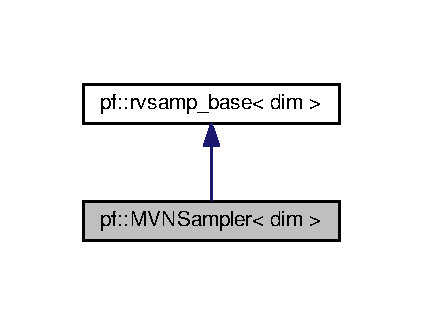
\includegraphics[width=203pt]{classpf_1_1MVNSampler__inherit__graph}
\end{center}
\end{figure}


Collaboration diagram for pf\+:\+:M\+V\+N\+Sampler$<$ dim $>$\+:\nopagebreak
\begin{figure}[H]
\begin{center}
\leavevmode
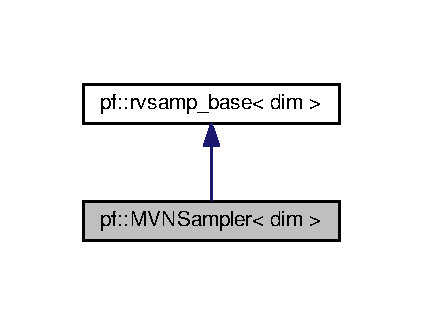
\includegraphics[width=203pt]{classpf_1_1MVNSampler__coll__graph}
\end{center}
\end{figure}
\subsection*{Public Types}
\begin{DoxyCompactItemize}
\item 
using \hyperlink{classpf_1_1MVNSampler_a70fb0813dd4b02e0563512c34079fee3}{Vec} = Eigen\+::\+Matrix$<$ double, dim, 1 $>$
\item 
using \hyperlink{classpf_1_1MVNSampler_a5bd837d18f475be7d0495470b6198a46}{Mat} = Eigen\+::\+Matrix$<$ double, dim, dim $>$
\end{DoxyCompactItemize}
\subsection*{Public Member Functions}
\begin{DoxyCompactItemize}
\item 
\hyperlink{classpf_1_1MVNSampler_ab7e165696c75108d6898db6ef0b60ac1}{M\+V\+N\+Sampler} ()
\begin{DoxyCompactList}\small\item\em Default-\/constructor sets up for multivariate standard Normal random variate generation. \end{DoxyCompactList}\item 
\hyperlink{classpf_1_1MVNSampler_a5756c28661b82c6cabd70bf023fd98b0}{M\+V\+N\+Sampler} (const \hyperlink{classpf_1_1MVNSampler_a70fb0813dd4b02e0563512c34079fee3}{Vec} \&mean\+Vec, const \hyperlink{classpf_1_1MVNSampler_a5bd837d18f475be7d0495470b6198a46}{Mat} \&cov\+Mat)
\begin{DoxyCompactList}\small\item\em The user must supply both mean and covariance matrix. \end{DoxyCompactList}\item 
void \hyperlink{classpf_1_1MVNSampler_a756c9b3cfd59f9a20f2f6568d9661695}{set\+Covar} (const \hyperlink{classpf_1_1MVNSampler_a5bd837d18f475be7d0495470b6198a46}{Mat} \&cov\+Mat)
\begin{DoxyCompactList}\small\item\em sets the covariance matrix of the sampler. \end{DoxyCompactList}\item 
void \hyperlink{classpf_1_1MVNSampler_a4dc0dbf7600f0f0b0087472baf8e56bc}{set\+Mean} (const \hyperlink{classpf_1_1MVNSampler_a70fb0813dd4b02e0563512c34079fee3}{Vec} \&mean\+Vec)
\begin{DoxyCompactList}\small\item\em sets the mean vector of the sampler. \end{DoxyCompactList}\item 
auto \hyperlink{classpf_1_1MVNSampler_a46bec6774945981d53c07c5145ce46d8}{sample} () -\/$>$ \hyperlink{classpf_1_1MVNSampler_a70fb0813dd4b02e0563512c34079fee3}{Vec}
\begin{DoxyCompactList}\small\item\em Draws a random vector. \end{DoxyCompactList}\end{DoxyCompactItemize}
\subsection*{Private Attributes}
\begin{DoxyCompactItemize}
\item 
std\+::normal\+\_\+distribution \hyperlink{classpf_1_1MVNSampler_aeceedd415d59b513914d29410488caa9}{m\+\_\+z\+\_\+gen}\hypertarget{classpf_1_1MVNSampler_aeceedd415d59b513914d29410488caa9}{}\label{classpf_1_1MVNSampler_aeceedd415d59b513914d29410488caa9}

\begin{DoxyCompactList}\small\item\em makes normal random variates \end{DoxyCompactList}\item 
\hyperlink{classpf_1_1MVNSampler_a5bd837d18f475be7d0495470b6198a46}{Mat} \hyperlink{classpf_1_1MVNSampler_a6f12200aa3bb97e0e91fd6f69597015a}{m\+\_\+scale\+\_\+mat}\hypertarget{classpf_1_1MVNSampler_a6f12200aa3bb97e0e91fd6f69597015a}{}\label{classpf_1_1MVNSampler_a6f12200aa3bb97e0e91fd6f69597015a}

\begin{DoxyCompactList}\small\item\em covariance matrix \end{DoxyCompactList}\item 
\hyperlink{classpf_1_1MVNSampler_a70fb0813dd4b02e0563512c34079fee3}{Vec} \hyperlink{classpf_1_1MVNSampler_a55453f92155dbe5499669a9c86d146c3}{m\+\_\+mean}\hypertarget{classpf_1_1MVNSampler_a55453f92155dbe5499669a9c86d146c3}{}\label{classpf_1_1MVNSampler_a55453f92155dbe5499669a9c86d146c3}

\begin{DoxyCompactList}\small\item\em mean vector \end{DoxyCompactList}\end{DoxyCompactItemize}
\subsection*{Additional Inherited Members}


\subsection{Detailed Description}
\subsubsection*{template$<$size\+\_\+t dim$>$\\*
class pf\+::\+M\+V\+N\+Sampler$<$ dim $>$}

A class that performs sampling from a multivariate normal distribution. 

\begin{DoxyAuthor}{Author}
taylor 
\end{DoxyAuthor}


\subsection{Member Typedef Documentation}
\index{pf\+::\+M\+V\+N\+Sampler@{pf\+::\+M\+V\+N\+Sampler}!Mat@{Mat}}
\index{Mat@{Mat}!pf\+::\+M\+V\+N\+Sampler@{pf\+::\+M\+V\+N\+Sampler}}
\subsubsection[{\texorpdfstring{Mat}{Mat}}]{\setlength{\rightskip}{0pt plus 5cm}template$<$size\+\_\+t dim$>$ using {\bf pf\+::\+M\+V\+N\+Sampler}$<$ dim $>$\+::{\bf Mat} =  Eigen\+::\+Matrix$<$double,dim,dim$>$}\hypertarget{classpf_1_1MVNSampler_a5bd837d18f475be7d0495470b6198a46}{}\label{classpf_1_1MVNSampler_a5bd837d18f475be7d0495470b6198a46}
type alias for linear algebra stuff \index{pf\+::\+M\+V\+N\+Sampler@{pf\+::\+M\+V\+N\+Sampler}!Vec@{Vec}}
\index{Vec@{Vec}!pf\+::\+M\+V\+N\+Sampler@{pf\+::\+M\+V\+N\+Sampler}}
\subsubsection[{\texorpdfstring{Vec}{Vec}}]{\setlength{\rightskip}{0pt plus 5cm}template$<$size\+\_\+t dim$>$ using {\bf pf\+::\+M\+V\+N\+Sampler}$<$ dim $>$\+::{\bf Vec} =  Eigen\+::\+Matrix$<$double,dim,1$>$}\hypertarget{classpf_1_1MVNSampler_a70fb0813dd4b02e0563512c34079fee3}{}\label{classpf_1_1MVNSampler_a70fb0813dd4b02e0563512c34079fee3}
type alias for linear algebra stuff 

\subsection{Constructor \& Destructor Documentation}
\index{pf\+::\+M\+V\+N\+Sampler@{pf\+::\+M\+V\+N\+Sampler}!M\+V\+N\+Sampler@{M\+V\+N\+Sampler}}
\index{M\+V\+N\+Sampler@{M\+V\+N\+Sampler}!pf\+::\+M\+V\+N\+Sampler@{pf\+::\+M\+V\+N\+Sampler}}
\subsubsection[{\texorpdfstring{M\+V\+N\+Sampler()}{MVNSampler()}}]{\setlength{\rightskip}{0pt plus 5cm}template$<$size\+\_\+t dim$>$ {\bf pf\+::\+M\+V\+N\+Sampler}$<$ dim $>$\+::{\bf M\+V\+N\+Sampler} (
\begin{DoxyParamCaption}
{}
\end{DoxyParamCaption}
)}\hypertarget{classpf_1_1MVNSampler_ab7e165696c75108d6898db6ef0b60ac1}{}\label{classpf_1_1MVNSampler_ab7e165696c75108d6898db6ef0b60ac1}


Default-\/constructor sets up for multivariate standard Normal random variate generation. 

\begin{DoxyRefDesc}{Todo}
\item[\hyperlink{todo__todo000003}{Todo}]\+: implement move semantics \end{DoxyRefDesc}
\index{pf\+::\+M\+V\+N\+Sampler@{pf\+::\+M\+V\+N\+Sampler}!M\+V\+N\+Sampler@{M\+V\+N\+Sampler}}
\index{M\+V\+N\+Sampler@{M\+V\+N\+Sampler}!pf\+::\+M\+V\+N\+Sampler@{pf\+::\+M\+V\+N\+Sampler}}
\subsubsection[{\texorpdfstring{M\+V\+N\+Sampler(const Vec \&mean\+Vec, const Mat \&cov\+Mat)}{MVNSampler(const Vec &meanVec, const Mat &covMat)}}]{\setlength{\rightskip}{0pt plus 5cm}template$<$size\+\_\+t dim$>$ {\bf pf\+::\+M\+V\+N\+Sampler}$<$ dim $>$\+::{\bf M\+V\+N\+Sampler} (
\begin{DoxyParamCaption}
\item[{const {\bf Vec} \&}]{mean\+Vec, }
\item[{const {\bf Mat} \&}]{cov\+Mat}
\end{DoxyParamCaption}
)}\hypertarget{classpf_1_1MVNSampler_a5756c28661b82c6cabd70bf023fd98b0}{}\label{classpf_1_1MVNSampler_a5756c28661b82c6cabd70bf023fd98b0}


The user must supply both mean and covariance matrix. 


\begin{DoxyParams}{Parameters}
{\em mean\+Vec} & a Vec for the mean vector of the sampling distribution. \\
\hline
{\em cov\+Mat} & a Mat representing the covariance matrix of the samples. \\
\hline
\end{DoxyParams}


\subsection{Member Function Documentation}
\index{pf\+::\+M\+V\+N\+Sampler@{pf\+::\+M\+V\+N\+Sampler}!sample@{sample}}
\index{sample@{sample}!pf\+::\+M\+V\+N\+Sampler@{pf\+::\+M\+V\+N\+Sampler}}
\subsubsection[{\texorpdfstring{sample() -\/$>$ Vec}{sample() -> Vec}}]{\setlength{\rightskip}{0pt plus 5cm}template$<$size\+\_\+t dim$>$ auto {\bf pf\+::\+M\+V\+N\+Sampler}$<$ dim $>$\+::sample (
\begin{DoxyParamCaption}
{}
\end{DoxyParamCaption}
) -\/$>$ {\bf Vec}}\hypertarget{classpf_1_1MVNSampler_a46bec6774945981d53c07c5145ce46d8}{}\label{classpf_1_1MVNSampler_a46bec6774945981d53c07c5145ce46d8}


Draws a random vector. 

\begin{DoxyReturn}{Returns}
a Vec random sample. 
\end{DoxyReturn}
\index{pf\+::\+M\+V\+N\+Sampler@{pf\+::\+M\+V\+N\+Sampler}!set\+Covar@{set\+Covar}}
\index{set\+Covar@{set\+Covar}!pf\+::\+M\+V\+N\+Sampler@{pf\+::\+M\+V\+N\+Sampler}}
\subsubsection[{\texorpdfstring{set\+Covar(const Mat \&cov\+Mat)}{setCovar(const Mat &covMat)}}]{\setlength{\rightskip}{0pt plus 5cm}template$<$size\+\_\+t dim$>$ void {\bf pf\+::\+M\+V\+N\+Sampler}$<$ dim $>$\+::set\+Covar (
\begin{DoxyParamCaption}
\item[{const {\bf Mat} \&}]{cov\+Mat}
\end{DoxyParamCaption}
)}\hypertarget{classpf_1_1MVNSampler_a756c9b3cfd59f9a20f2f6568d9661695}{}\label{classpf_1_1MVNSampler_a756c9b3cfd59f9a20f2f6568d9661695}


sets the covariance matrix of the sampler. 


\begin{DoxyParams}{Parameters}
{\em cov\+Mat} & the desired covariance matrix. \\
\hline
\end{DoxyParams}
\index{pf\+::\+M\+V\+N\+Sampler@{pf\+::\+M\+V\+N\+Sampler}!set\+Mean@{set\+Mean}}
\index{set\+Mean@{set\+Mean}!pf\+::\+M\+V\+N\+Sampler@{pf\+::\+M\+V\+N\+Sampler}}
\subsubsection[{\texorpdfstring{set\+Mean(const Vec \&mean\+Vec)}{setMean(const Vec &meanVec)}}]{\setlength{\rightskip}{0pt plus 5cm}template$<$size\+\_\+t dim$>$ void {\bf pf\+::\+M\+V\+N\+Sampler}$<$ dim $>$\+::set\+Mean (
\begin{DoxyParamCaption}
\item[{const {\bf Vec} \&}]{mean\+Vec}
\end{DoxyParamCaption}
)}\hypertarget{classpf_1_1MVNSampler_a4dc0dbf7600f0f0b0087472baf8e56bc}{}\label{classpf_1_1MVNSampler_a4dc0dbf7600f0f0b0087472baf8e56bc}


sets the mean vector of the sampler. 


\begin{DoxyParams}{Parameters}
{\em mean\+Vec} & the desired mean vector. \\
\hline
\end{DoxyParams}


The documentation for this class was generated from the following file\+:\begin{DoxyCompactItemize}
\item 
include/\hyperlink{rv__samp_8h}{rv\+\_\+samp.\+h}\end{DoxyCompactItemize}

\hypertarget{classpf_1_1rbase}{}\section{pf\+:\+:rbase$<$ nparts, dimx $>$ Class Template Reference}
\label{classpf_1_1rbase}\index{pf\+::rbase$<$ nparts, dimx $>$@{pf\+::rbase$<$ nparts, dimx $>$}}


Base class for all resampler types.  




{\ttfamily \#include $<$resamplers.\+h$>$}



Inheritance diagram for pf\+:\+:rbase$<$ nparts, dimx $>$\+:\nopagebreak
\begin{figure}[H]
\begin{center}
\leavevmode
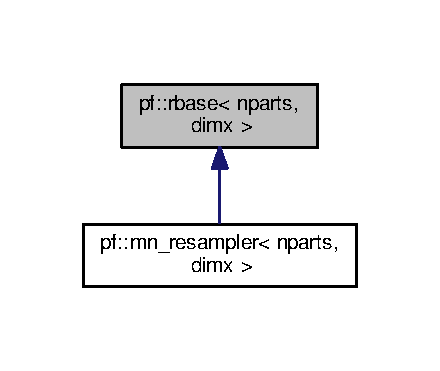
\includegraphics[width=211pt]{classpf_1_1rbase__inherit__graph}
\end{center}
\end{figure}
\subsection*{Public Types}
\begin{DoxyCompactItemize}
\item 
using \hyperlink{classpf_1_1rbase_a47a4bdc0e3c08b72ce4f24a18d5b0e04}{ssv} = Eigen\+::\+Matrix$<$ double, dimx, 1 $>$
\item 
using \hyperlink{classpf_1_1rbase_a89951bb3872c1c6a0c3da0962a9aaa13}{array\+Vec} = std\+::array$<$ \hyperlink{classpf_1_1rbase_a47a4bdc0e3c08b72ce4f24a18d5b0e04}{ssv}, nparts $>$
\item 
using \hyperlink{classpf_1_1rbase_a37b2d02d00f75d9550122b763cbb3fed}{array\+Double} = std\+::array$<$ double, nparts $>$
\end{DoxyCompactItemize}
\subsection*{Public Member Functions}
\begin{DoxyCompactItemize}
\item 
\hyperlink{classpf_1_1rbase_af43b8b8246426cd4f69a73784763bf95}{rbase} ()\hypertarget{classpf_1_1rbase_af43b8b8246426cd4f69a73784763bf95}{}\label{classpf_1_1rbase_af43b8b8246426cd4f69a73784763bf95}

\begin{DoxyCompactList}\small\item\em The default constructor. This is the only option available. Sets the seed with the clock. \end{DoxyCompactList}\item 
virtual void \hyperlink{classpf_1_1rbase_a0d8136638281a96a8c01b07393af9fc8}{resamp\+Log\+Wts} (\hyperlink{classpf_1_1rbase_a89951bb3872c1c6a0c3da0962a9aaa13}{array\+Vec} \&old\+Parts, \hyperlink{classpf_1_1rbase_a37b2d02d00f75d9550122b763cbb3fed}{array\+Double} \&old\+Log\+Un\+Norm\+Wts)=0
\begin{DoxyCompactList}\small\item\em Function to resample from log unnormalized weights. \end{DoxyCompactList}\end{DoxyCompactItemize}
\subsection*{Private Attributes}
\begin{DoxyCompactItemize}
\item 
std\+::mt19937 \hyperlink{classpf_1_1rbase_ad526b252f1ee84fc24b6ace422c1b482}{m\+\_\+gen}\hypertarget{classpf_1_1rbase_ad526b252f1ee84fc24b6ace422c1b482}{}\label{classpf_1_1rbase_ad526b252f1ee84fc24b6ace422c1b482}

\begin{DoxyCompactList}\small\item\em prng \end{DoxyCompactList}\end{DoxyCompactItemize}


\subsection{Detailed Description}
\subsubsection*{template$<$size\+\_\+t nparts, size\+\_\+t dimx$>$\\*
class pf\+::rbase$<$ nparts, dimx $>$}

Base class for all resampler types. 

\begin{DoxyAuthor}{Author}
taylor 
\end{DoxyAuthor}
\begin{DoxyDate}{Date}
15/04/18 
\end{DoxyDate}


\subsection{Member Typedef Documentation}
\index{pf\+::rbase@{pf\+::rbase}!array\+Double@{array\+Double}}
\index{array\+Double@{array\+Double}!pf\+::rbase@{pf\+::rbase}}
\subsubsection[{\texorpdfstring{array\+Double}{arrayDouble}}]{\setlength{\rightskip}{0pt plus 5cm}template$<$size\+\_\+t nparts, size\+\_\+t dimx$>$ using {\bf pf\+::rbase}$<$ nparts, dimx $>$\+::{\bf array\+Double} =  std\+::array$<$double,nparts$>$}\hypertarget{classpf_1_1rbase_a37b2d02d00f75d9550122b763cbb3fed}{}\label{classpf_1_1rbase_a37b2d02d00f75d9550122b763cbb3fed}
type alias for array of doubles \index{pf\+::rbase@{pf\+::rbase}!array\+Vec@{array\+Vec}}
\index{array\+Vec@{array\+Vec}!pf\+::rbase@{pf\+::rbase}}
\subsubsection[{\texorpdfstring{array\+Vec}{arrayVec}}]{\setlength{\rightskip}{0pt plus 5cm}template$<$size\+\_\+t nparts, size\+\_\+t dimx$>$ using {\bf pf\+::rbase}$<$ nparts, dimx $>$\+::{\bf array\+Vec} =  std\+::array$<${\bf ssv}, nparts$>$}\hypertarget{classpf_1_1rbase_a89951bb3872c1c6a0c3da0962a9aaa13}{}\label{classpf_1_1rbase_a89951bb3872c1c6a0c3da0962a9aaa13}
type alias for array of Eigen Matrices \index{pf\+::rbase@{pf\+::rbase}!ssv@{ssv}}
\index{ssv@{ssv}!pf\+::rbase@{pf\+::rbase}}
\subsubsection[{\texorpdfstring{ssv}{ssv}}]{\setlength{\rightskip}{0pt plus 5cm}template$<$size\+\_\+t nparts, size\+\_\+t dimx$>$ using {\bf pf\+::rbase}$<$ nparts, dimx $>$\+::{\bf ssv} =  Eigen\+::\+Matrix$<$double,dimx,1$>$}\hypertarget{classpf_1_1rbase_a47a4bdc0e3c08b72ce4f24a18d5b0e04}{}\label{classpf_1_1rbase_a47a4bdc0e3c08b72ce4f24a18d5b0e04}
type alias for linear algebra stuff 

\subsection{Member Function Documentation}
\index{pf\+::rbase@{pf\+::rbase}!resamp\+Log\+Wts@{resamp\+Log\+Wts}}
\index{resamp\+Log\+Wts@{resamp\+Log\+Wts}!pf\+::rbase@{pf\+::rbase}}
\subsubsection[{\texorpdfstring{resamp\+Log\+Wts(array\+Vec \&old\+Parts, array\+Double \&old\+Log\+Un\+Norm\+Wts)=0}{resampLogWts(arrayVec &oldParts, arrayDouble &oldLogUnNormWts)=0}}]{\setlength{\rightskip}{0pt plus 5cm}template$<$size\+\_\+t nparts, size\+\_\+t dimx$>$ virtual void {\bf pf\+::rbase}$<$ nparts, dimx $>$\+::resamp\+Log\+Wts (
\begin{DoxyParamCaption}
\item[{{\bf array\+Vec} \&}]{old\+Parts, }
\item[{{\bf array\+Double} \&}]{old\+Log\+Un\+Norm\+Wts}
\end{DoxyParamCaption}
)\hspace{0.3cm}{\ttfamily [pure virtual]}}\hypertarget{classpf_1_1rbase_a0d8136638281a96a8c01b07393af9fc8}{}\label{classpf_1_1rbase_a0d8136638281a96a8c01b07393af9fc8}


Function to resample from log unnormalized weights. 


\begin{DoxyParams}{Parameters}
{\em old\+Parts} & \\
\hline
{\em old\+Log\+Un\+Norm\+Wts} & \\
\hline
\end{DoxyParams}


Implemented in \hyperlink{classpf_1_1mn__resampler_a9fe1aa27517fc0333f2fa82653a4d9fc}{pf\+::mn\+\_\+resampler$<$ nparts, dimx $>$}.



The documentation for this class was generated from the following file\+:\begin{DoxyCompactItemize}
\item 
include/\hyperlink{resamplers_8h}{resamplers.\+h}\end{DoxyCompactItemize}

\hypertarget{classpf_1_1rvsamp__base}{}\section{pf\+:\+:rvsamp\+\_\+base$<$ dim $>$ Class Template Reference}
\label{classpf_1_1rvsamp__base}\index{pf\+::rvsamp\+\_\+base$<$ dim $>$@{pf\+::rvsamp\+\_\+base$<$ dim $>$}}


Base class for all random variable sampler types. Primary benefit is that it sets the seed for you.  




{\ttfamily \#include $<$rv\+\_\+samp.\+h$>$}



Inheritance diagram for pf\+:\+:rvsamp\+\_\+base$<$ dim $>$\+:\nopagebreak
\begin{figure}[H]
\begin{center}
\leavevmode
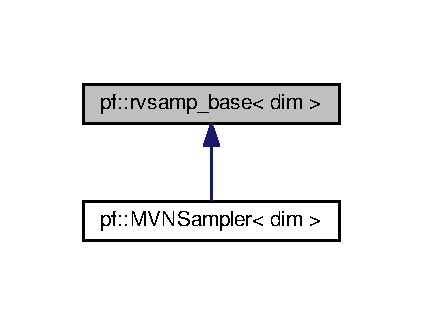
\includegraphics[width=203pt]{classpf_1_1rvsamp__base__inherit__graph}
\end{center}
\end{figure}
\subsection*{Public Types}
\begin{DoxyCompactItemize}
\item 
using \hyperlink{classpf_1_1rvsamp__base_a5d22b5297cc9ec74dfbc500b76e6747d}{ssv} = Eigen\+::\+Matrix$<$ double, dim, 1 $>$
\end{DoxyCompactItemize}
\subsection*{Public Member Functions}
\begin{DoxyCompactItemize}
\item 
\hyperlink{classpf_1_1rvsamp__base_a72abf1777cf753aa58f2b753232d864f}{rvsamp\+\_\+base} ()\hypertarget{classpf_1_1rvsamp__base_a72abf1777cf753aa58f2b753232d864f}{}\label{classpf_1_1rvsamp__base_a72abf1777cf753aa58f2b753232d864f}

\begin{DoxyCompactList}\small\item\em The default constructor. This is the only option available. Sets the seed with the clock. \end{DoxyCompactList}\end{DoxyCompactItemize}
\subsection*{Protected Attributes}
\begin{DoxyCompactItemize}
\item 
std\+::mt19937 \hyperlink{classpf_1_1rvsamp__base_ab24a599151b7ad0836ddee218b1941a1}{m\+\_\+rng}\hypertarget{classpf_1_1rvsamp__base_ab24a599151b7ad0836ddee218b1941a1}{}\label{classpf_1_1rvsamp__base_ab24a599151b7ad0836ddee218b1941a1}

\begin{DoxyCompactList}\small\item\em prng \end{DoxyCompactList}\end{DoxyCompactItemize}


\subsection{Detailed Description}
\subsubsection*{template$<$size\+\_\+t dim = 1$>$\\*
class pf\+::rvsamp\+\_\+base$<$ dim $>$}

Base class for all random variable sampler types. Primary benefit is that it sets the seed for you. 

\begin{DoxyAuthor}{Author}
taylor 
\end{DoxyAuthor}


\subsection{Member Typedef Documentation}
\index{pf\+::rvsamp\+\_\+base@{pf\+::rvsamp\+\_\+base}!ssv@{ssv}}
\index{ssv@{ssv}!pf\+::rvsamp\+\_\+base@{pf\+::rvsamp\+\_\+base}}
\subsubsection[{\texorpdfstring{ssv}{ssv}}]{\setlength{\rightskip}{0pt plus 5cm}template$<$size\+\_\+t dim = 1$>$ using {\bf pf\+::rvsamp\+\_\+base}$<$ dim $>$\+::{\bf ssv} =  Eigen\+::\+Matrix$<$double,dim,1$>$}\hypertarget{classpf_1_1rvsamp__base_a5d22b5297cc9ec74dfbc500b76e6747d}{}\label{classpf_1_1rvsamp__base_a5d22b5297cc9ec74dfbc500b76e6747d}
\char`\"{}state size vector\char`\"{} type alias for linear algebra stuff 

The documentation for this class was generated from the following file\+:\begin{DoxyCompactItemize}
\item 
include/\hyperlink{rv__samp_8h}{rv\+\_\+samp.\+h}\end{DoxyCompactItemize}

\hypertarget{classSISRFilter}{}\section{S\+I\+S\+R\+Filter$<$ nparts, dimx, dimy, resamp\+\_\+t, float\+\_\+t $>$ Class Template Reference}
\label{classSISRFilter}\index{S\+I\+S\+R\+Filter$<$ nparts, dimx, dimy, resamp\+\_\+t, float\+\_\+t $>$@{S\+I\+S\+R\+Filter$<$ nparts, dimx, dimy, resamp\+\_\+t, float\+\_\+t $>$}}


A base class for the Sequential Important Sampling with Resampling (S\+I\+SR).  




{\ttfamily \#include $<$sisr\+\_\+filter.\+h$>$}



Inheritance diagram for S\+I\+S\+R\+Filter$<$ nparts, dimx, dimy, resamp\+\_\+t, float\+\_\+t $>$\+:\nopagebreak
\begin{figure}[H]
\begin{center}
\leavevmode
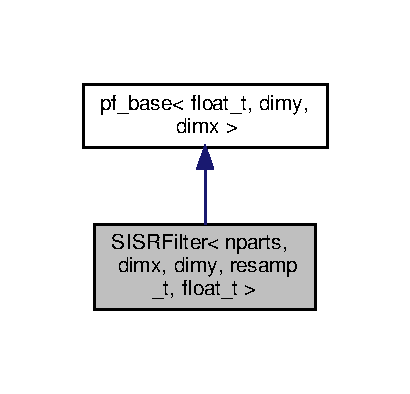
\includegraphics[width=197pt]{classSISRFilter__inherit__graph}
\end{center}
\end{figure}


Collaboration diagram for S\+I\+S\+R\+Filter$<$ nparts, dimx, dimy, resamp\+\_\+t, float\+\_\+t $>$\+:\nopagebreak
\begin{figure}[H]
\begin{center}
\leavevmode
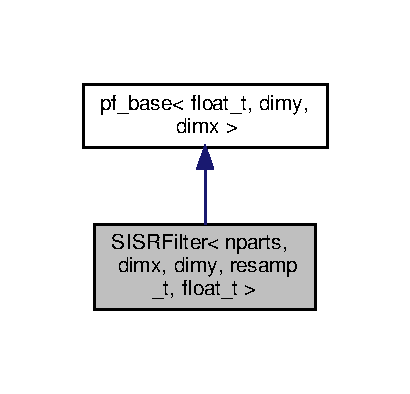
\includegraphics[width=197pt]{classSISRFilter__coll__graph}
\end{center}
\end{figure}
\subsection*{Public Types}
\begin{DoxyCompactItemize}
\item 
using \hyperlink{classSISRFilter_abfec45cf57ea6fadae4a9da8b0042351}{ssv} = Eigen\+::\+Matrix$<$ float\+\_\+t, dimx, 1 $>$
\item 
using \hyperlink{classSISRFilter_a5b762e9352857a9e48db3932191887ef}{osv} = Eigen\+::\+Matrix$<$ float\+\_\+t, dimy, 1 $>$
\item 
using \hyperlink{classSISRFilter_a7355e966778c788dfe227ef5254677c4}{Mat} = Eigen\+::\+Matrix$<$ float\+\_\+t, Eigen\+::\+Dynamic, Eigen\+::\+Dynamic $>$
\item 
using \hyperlink{classSISRFilter_a5c8a38ceb31c22f3c3f38b0ead5c1ce7}{array\+States} = std\+::array$<$ \hyperlink{classSISRFilter_abfec45cf57ea6fadae4a9da8b0042351}{ssv}, nparts $>$
\item 
using \hyperlink{classSISRFilter_a35f5a590324bd78fc4f6ded236937ac2}{arrayfloat\+\_\+t} = std\+::array$<$ float\+\_\+t, nparts $>$
\end{DoxyCompactItemize}
\subsection*{Public Member Functions}
\begin{DoxyCompactItemize}
\item 
\hyperlink{classSISRFilter_a46243d4a5ef93f3762d1130fa4d43389}{S\+I\+S\+R\+Filter} (const unsigned int \&rs=1)
\begin{DoxyCompactList}\small\item\em The (one and only) constructor. \end{DoxyCompactList}\item 
\mbox{\Hypertarget{classSISRFilter_a0934886c2ab47682364e3624c24be874}\label{classSISRFilter_a0934886c2ab47682364e3624c24be874}} 
virtual \hyperlink{classSISRFilter_a0934886c2ab47682364e3624c24be874}{$\sim$\+S\+I\+S\+R\+Filter} ()
\begin{DoxyCompactList}\small\item\em The (virtual) destructor. \end{DoxyCompactList}\item 
float\+\_\+t \hyperlink{classSISRFilter_a48bdb88b2ed4041ab6d8a6547703ebf3}{get\+Log\+Cond\+Like} () const
\begin{DoxyCompactList}\small\item\em Returns the most recent (log-\/) conditiona likelihood. \end{DoxyCompactList}\item 
std\+::vector$<$ \hyperlink{classSISRFilter_a7355e966778c788dfe227ef5254677c4}{Mat} $>$ \hyperlink{classSISRFilter_a88ef9409ded3ec7e6745e184daad86c4}{get\+Expectations} () const
\begin{DoxyCompactList}\small\item\em return all stored expectations (taken with respect to \$p(x\+\_\+t$\vert$y\+\_\+\{1\+:t\})\$ \end{DoxyCompactList}\item 
void \hyperlink{classSISRFilter_a0fd4ac5135ff9a4bb32a286533855197}{filter} (const \hyperlink{classSISRFilter_a5b762e9352857a9e48db3932191887ef}{osv} \&data, const std\+::vector$<$ std\+::function$<$ const \hyperlink{classSISRFilter_a7355e966778c788dfe227ef5254677c4}{Mat}(const \hyperlink{classSISRFilter_abfec45cf57ea6fadae4a9da8b0042351}{ssv} \&)$>$ $>$ \&fs=std\+::vector$<$ std\+::function$<$ const \hyperlink{classSISRFilter_a7355e966778c788dfe227ef5254677c4}{Mat}(const \hyperlink{classSISRFilter_abfec45cf57ea6fadae4a9da8b0042351}{ssv} \&)$>$ $>$())
\begin{DoxyCompactList}\small\item\em updates filtering distribution on a new datapoint. Optionally stores expectations of functionals. \end{DoxyCompactList}\item 
virtual float\+\_\+t \hyperlink{classSISRFilter_aff620e2208b6b26bbe109ce05520c5f8}{log\+Mu\+Ev} (const \hyperlink{classSISRFilter_abfec45cf57ea6fadae4a9da8b0042351}{ssv} \&x1)=0
\begin{DoxyCompactList}\small\item\em Calculate mu\+Ev or logmu\+Ev. \end{DoxyCompactList}\item 
virtual \hyperlink{classSISRFilter_abfec45cf57ea6fadae4a9da8b0042351}{ssv} \hyperlink{classSISRFilter_aac34adbf022dad8b62470de35c5ceb17}{q1\+Samp} (const \hyperlink{classSISRFilter_a5b762e9352857a9e48db3932191887ef}{osv} \&y1)=0
\begin{DoxyCompactList}\small\item\em Samples from time 1 proposal. \end{DoxyCompactList}\item 
virtual float\+\_\+t \hyperlink{classSISRFilter_a21d5130f35d1d5c21b697ca7ea8e9d83}{log\+Q1\+Ev} (const \hyperlink{classSISRFilter_abfec45cf57ea6fadae4a9da8b0042351}{ssv} \&x1, const \hyperlink{classSISRFilter_a5b762e9352857a9e48db3932191887ef}{osv} \&y1)=0
\begin{DoxyCompactList}\small\item\em Calculate q1\+Ev or log q1\+Ev. \end{DoxyCompactList}\item 
virtual float\+\_\+t \hyperlink{classSISRFilter_a73fe8481e4cb40142544c04823851aa8}{log\+G\+Ev} (const \hyperlink{classSISRFilter_a5b762e9352857a9e48db3932191887ef}{osv} \&yt, const \hyperlink{classSISRFilter_abfec45cf57ea6fadae4a9da8b0042351}{ssv} \&xt)=0
\begin{DoxyCompactList}\small\item\em Calculate g\+Ev or log\+G\+Ev. \end{DoxyCompactList}\item 
virtual float\+\_\+t \hyperlink{classSISRFilter_a7aa1e90a0b641728d5f8d7bd8c699ba8}{log\+F\+Ev} (const \hyperlink{classSISRFilter_abfec45cf57ea6fadae4a9da8b0042351}{ssv} \&xt, const \hyperlink{classSISRFilter_abfec45cf57ea6fadae4a9da8b0042351}{ssv} \&xtm1)=0
\begin{DoxyCompactList}\small\item\em Evaluates the state transition density. \end{DoxyCompactList}\item 
virtual \hyperlink{classSISRFilter_abfec45cf57ea6fadae4a9da8b0042351}{ssv} \hyperlink{classSISRFilter_a609bb361da16e1b24ebfab693620241b}{q\+Samp} (const \hyperlink{classSISRFilter_abfec45cf57ea6fadae4a9da8b0042351}{ssv} \&xtm1, const \hyperlink{classSISRFilter_a5b762e9352857a9e48db3932191887ef}{osv} \&yt)=0
\begin{DoxyCompactList}\small\item\em Samples from the proposal/instrumental/importance density at time t. \end{DoxyCompactList}\item 
virtual float\+\_\+t \hyperlink{classSISRFilter_a4edca9291a3a118c37bd0e41c06fb7da}{log\+Q\+Ev} (const \hyperlink{classSISRFilter_abfec45cf57ea6fadae4a9da8b0042351}{ssv} \&xt, const \hyperlink{classSISRFilter_abfec45cf57ea6fadae4a9da8b0042351}{ssv} \&xtm1, const \hyperlink{classSISRFilter_a5b762e9352857a9e48db3932191887ef}{osv} \&yt)=0
\begin{DoxyCompactList}\small\item\em Evaluates the proposal/instrumental/importance density/pmf. \end{DoxyCompactList}\end{DoxyCompactItemize}
\subsection*{Private Attributes}
\begin{DoxyCompactItemize}
\item 
\mbox{\Hypertarget{classSISRFilter_a98c87c50c054354cdc85dc800ba15bdd}\label{classSISRFilter_a98c87c50c054354cdc85dc800ba15bdd}} 
\hyperlink{classSISRFilter_a5c8a38ceb31c22f3c3f38b0ead5c1ce7}{array\+States} \hyperlink{classSISRFilter_a98c87c50c054354cdc85dc800ba15bdd}{m\+\_\+particles}
\begin{DoxyCompactList}\small\item\em particle samples \end{DoxyCompactList}\item 
\mbox{\Hypertarget{classSISRFilter_a99f63cbae203084cf3d812a61bb725fe}\label{classSISRFilter_a99f63cbae203084cf3d812a61bb725fe}} 
\hyperlink{classSISRFilter_a35f5a590324bd78fc4f6ded236937ac2}{arrayfloat\+\_\+t} \hyperlink{classSISRFilter_a99f63cbae203084cf3d812a61bb725fe}{m\+\_\+log\+Un\+Norm\+Weights}
\begin{DoxyCompactList}\small\item\em particle weights \end{DoxyCompactList}\item 
\mbox{\Hypertarget{classSISRFilter_a1aafd7da52826fd25967c8258f68ce9c}\label{classSISRFilter_a1aafd7da52826fd25967c8258f68ce9c}} 
unsigned int \hyperlink{classSISRFilter_a1aafd7da52826fd25967c8258f68ce9c}{m\+\_\+now}
\begin{DoxyCompactList}\small\item\em current time point \end{DoxyCompactList}\item 
\mbox{\Hypertarget{classSISRFilter_a7031db4bd7d9c1db7ea83150893525ed}\label{classSISRFilter_a7031db4bd7d9c1db7ea83150893525ed}} 
float\+\_\+t \hyperlink{classSISRFilter_a7031db4bd7d9c1db7ea83150893525ed}{m\+\_\+log\+Last\+Cond\+Like}
\begin{DoxyCompactList}\small\item\em log p(y\+\_\+t$\vert$y\+\_\+\{1\+:t-\/1\}) or log p(y1) \end{DoxyCompactList}\item 
\mbox{\Hypertarget{classSISRFilter_a46f945e550fab93eedddf10a69c251f1}\label{classSISRFilter_a46f945e550fab93eedddf10a69c251f1}} 
resamp\+\_\+t \hyperlink{classSISRFilter_a46f945e550fab93eedddf10a69c251f1}{m\+\_\+resampler}
\begin{DoxyCompactList}\small\item\em resampling object \end{DoxyCompactList}\item 
\mbox{\Hypertarget{classSISRFilter_acb5ed65aeed970afb929c108d04ee0d1}\label{classSISRFilter_acb5ed65aeed970afb929c108d04ee0d1}} 
std\+::vector$<$ \hyperlink{classSISRFilter_a7355e966778c788dfe227ef5254677c4}{Mat} $>$ \hyperlink{classSISRFilter_acb5ed65aeed970afb929c108d04ee0d1}{m\+\_\+expectations}
\begin{DoxyCompactList}\small\item\em expectations E\mbox{[}h(x\+\_\+t) $\vert$ y\+\_\+\{1\+:t\}\mbox{]} for user defined \char`\"{}h\char`\"{}s \end{DoxyCompactList}\item 
\mbox{\Hypertarget{classSISRFilter_a196049324b4c6c42a927d83f659619aa}\label{classSISRFilter_a196049324b4c6c42a927d83f659619aa}} 
unsigned int \hyperlink{classSISRFilter_a196049324b4c6c42a927d83f659619aa}{m\+\_\+resamp\+Sched}
\begin{DoxyCompactList}\small\item\em resampling schedule (e.\+g. resample every \+\_\+\+\_\+ time points) \end{DoxyCompactList}\end{DoxyCompactItemize}


\subsection{Detailed Description}
\subsubsection*{template$<$size\+\_\+t nparts, size\+\_\+t dimx, size\+\_\+t dimy, typename resamp\+\_\+t, typename float\+\_\+t$>$\newline
class S\+I\+S\+R\+Filter$<$ nparts, dimx, dimy, resamp\+\_\+t, float\+\_\+t $>$}

A base class for the Sequential Important Sampling with Resampling (S\+I\+SR). 

\begin{DoxyAuthor}{Author}
taylor 
\end{DoxyAuthor}


\subsection{Member Typedef Documentation}
\mbox{\Hypertarget{classSISRFilter_a35f5a590324bd78fc4f6ded236937ac2}\label{classSISRFilter_a35f5a590324bd78fc4f6ded236937ac2}} 
\index{S\+I\+S\+R\+Filter@{S\+I\+S\+R\+Filter}!arrayfloat\+\_\+t@{arrayfloat\+\_\+t}}
\index{arrayfloat\+\_\+t@{arrayfloat\+\_\+t}!S\+I\+S\+R\+Filter@{S\+I\+S\+R\+Filter}}
\subsubsection{\texorpdfstring{arrayfloat\+\_\+t}{arrayfloat\_t}}
{\footnotesize\ttfamily template$<$size\+\_\+t nparts, size\+\_\+t dimx, size\+\_\+t dimy, typename resamp\+\_\+t , typename float\+\_\+t $>$ \\
using \hyperlink{classSISRFilter}{S\+I\+S\+R\+Filter}$<$ nparts, dimx, dimy, resamp\+\_\+t, float\+\_\+t $>$\+::\hyperlink{classSISRFilter_a35f5a590324bd78fc4f6ded236937ac2}{arrayfloat\+\_\+t} =  std\+::array$<$float\+\_\+t, nparts$>$}

type alias for array of float\+\_\+ts \mbox{\Hypertarget{classSISRFilter_a5c8a38ceb31c22f3c3f38b0ead5c1ce7}\label{classSISRFilter_a5c8a38ceb31c22f3c3f38b0ead5c1ce7}} 
\index{S\+I\+S\+R\+Filter@{S\+I\+S\+R\+Filter}!array\+States@{array\+States}}
\index{array\+States@{array\+States}!S\+I\+S\+R\+Filter@{S\+I\+S\+R\+Filter}}
\subsubsection{\texorpdfstring{array\+States}{arrayStates}}
{\footnotesize\ttfamily template$<$size\+\_\+t nparts, size\+\_\+t dimx, size\+\_\+t dimy, typename resamp\+\_\+t , typename float\+\_\+t $>$ \\
using \hyperlink{classSISRFilter}{S\+I\+S\+R\+Filter}$<$ nparts, dimx, dimy, resamp\+\_\+t, float\+\_\+t $>$\+::\hyperlink{classSISRFilter_a5c8a38ceb31c22f3c3f38b0ead5c1ce7}{array\+States} =  std\+::array$<$\hyperlink{classSISRFilter_abfec45cf57ea6fadae4a9da8b0042351}{ssv}, nparts$>$}

type alias for linear algebra stuff \mbox{\Hypertarget{classSISRFilter_a7355e966778c788dfe227ef5254677c4}\label{classSISRFilter_a7355e966778c788dfe227ef5254677c4}} 
\index{S\+I\+S\+R\+Filter@{S\+I\+S\+R\+Filter}!Mat@{Mat}}
\index{Mat@{Mat}!S\+I\+S\+R\+Filter@{S\+I\+S\+R\+Filter}}
\subsubsection{\texorpdfstring{Mat}{Mat}}
{\footnotesize\ttfamily template$<$size\+\_\+t nparts, size\+\_\+t dimx, size\+\_\+t dimy, typename resamp\+\_\+t , typename float\+\_\+t $>$ \\
using \hyperlink{classSISRFilter}{S\+I\+S\+R\+Filter}$<$ nparts, dimx, dimy, resamp\+\_\+t, float\+\_\+t $>$\+::\hyperlink{classSISRFilter_a7355e966778c788dfe227ef5254677c4}{Mat} =  Eigen\+::\+Matrix$<$float\+\_\+t,Eigen\+::\+Dynamic,Eigen\+::\+Dynamic$>$}

type alias for linear algebra stuff \mbox{\Hypertarget{classSISRFilter_a5b762e9352857a9e48db3932191887ef}\label{classSISRFilter_a5b762e9352857a9e48db3932191887ef}} 
\index{S\+I\+S\+R\+Filter@{S\+I\+S\+R\+Filter}!osv@{osv}}
\index{osv@{osv}!S\+I\+S\+R\+Filter@{S\+I\+S\+R\+Filter}}
\subsubsection{\texorpdfstring{osv}{osv}}
{\footnotesize\ttfamily template$<$size\+\_\+t nparts, size\+\_\+t dimx, size\+\_\+t dimy, typename resamp\+\_\+t , typename float\+\_\+t $>$ \\
using \hyperlink{classSISRFilter}{S\+I\+S\+R\+Filter}$<$ nparts, dimx, dimy, resamp\+\_\+t, float\+\_\+t $>$\+::\hyperlink{classSISRFilter_a5b762e9352857a9e48db3932191887ef}{osv} =  Eigen\+::\+Matrix$<$float\+\_\+t, dimy, 1$>$}

\char`\"{}obs size vector\char`\"{} type alias for linear algebra stuff \mbox{\Hypertarget{classSISRFilter_abfec45cf57ea6fadae4a9da8b0042351}\label{classSISRFilter_abfec45cf57ea6fadae4a9da8b0042351}} 
\index{S\+I\+S\+R\+Filter@{S\+I\+S\+R\+Filter}!ssv@{ssv}}
\index{ssv@{ssv}!S\+I\+S\+R\+Filter@{S\+I\+S\+R\+Filter}}
\subsubsection{\texorpdfstring{ssv}{ssv}}
{\footnotesize\ttfamily template$<$size\+\_\+t nparts, size\+\_\+t dimx, size\+\_\+t dimy, typename resamp\+\_\+t , typename float\+\_\+t $>$ \\
using \hyperlink{classSISRFilter}{S\+I\+S\+R\+Filter}$<$ nparts, dimx, dimy, resamp\+\_\+t, float\+\_\+t $>$\+::\hyperlink{classSISRFilter_abfec45cf57ea6fadae4a9da8b0042351}{ssv} =  Eigen\+::\+Matrix$<$float\+\_\+t, dimx, 1$>$}

\char`\"{}state size vector\char`\"{} type alias for linear algebra stuff 

\subsection{Constructor \& Destructor Documentation}
\mbox{\Hypertarget{classSISRFilter_a46243d4a5ef93f3762d1130fa4d43389}\label{classSISRFilter_a46243d4a5ef93f3762d1130fa4d43389}} 
\index{S\+I\+S\+R\+Filter@{S\+I\+S\+R\+Filter}!S\+I\+S\+R\+Filter@{S\+I\+S\+R\+Filter}}
\index{S\+I\+S\+R\+Filter@{S\+I\+S\+R\+Filter}!S\+I\+S\+R\+Filter@{S\+I\+S\+R\+Filter}}
\subsubsection{\texorpdfstring{S\+I\+S\+R\+Filter()}{SISRFilter()}}
{\footnotesize\ttfamily template$<$size\+\_\+t nparts, size\+\_\+t dimx, size\+\_\+t dimy, typename resamp\+\_\+t , typename float\+\_\+t $>$ \\
\hyperlink{classSISRFilter}{S\+I\+S\+R\+Filter}$<$ nparts, dimx, dimy, resamp\+\_\+t, float\+\_\+t $>$\+::\hyperlink{classSISRFilter}{S\+I\+S\+R\+Filter} (\begin{DoxyParamCaption}\item[{const unsigned int \&}]{rs = {\ttfamily 1} }\end{DoxyParamCaption})}



The (one and only) constructor. 


\begin{DoxyParams}{Parameters}
{\em rs} & the resampling schedule (resample every rs time points). \\
\hline
\end{DoxyParams}


\subsection{Member Function Documentation}
\mbox{\Hypertarget{classSISRFilter_a0fd4ac5135ff9a4bb32a286533855197}\label{classSISRFilter_a0fd4ac5135ff9a4bb32a286533855197}} 
\index{S\+I\+S\+R\+Filter@{S\+I\+S\+R\+Filter}!filter@{filter}}
\index{filter@{filter}!S\+I\+S\+R\+Filter@{S\+I\+S\+R\+Filter}}
\subsubsection{\texorpdfstring{filter()}{filter()}}
{\footnotesize\ttfamily template$<$size\+\_\+t nparts, size\+\_\+t dimx, size\+\_\+t dimy, typename resamp\+\_\+t , typename float\+\_\+t $>$ \\
void \hyperlink{classSISRFilter}{S\+I\+S\+R\+Filter}$<$ nparts, dimx, dimy, resamp\+\_\+t, float\+\_\+t $>$\+::filter (\begin{DoxyParamCaption}\item[{const \hyperlink{classSISRFilter_a5b762e9352857a9e48db3932191887ef}{osv} \&}]{data,  }\item[{const std\+::vector$<$ std\+::function$<$ const \hyperlink{classSISRFilter_a7355e966778c788dfe227ef5254677c4}{Mat}(const \hyperlink{classSISRFilter_abfec45cf57ea6fadae4a9da8b0042351}{ssv} \&)$>$ $>$ \&}]{fs = {\ttfamily std\+:\+:vector$<$std\+:\+:function$<$const~\hyperlink{classSISRFilter_a7355e966778c788dfe227ef5254677c4}{Mat}(const~\hyperlink{classSISRFilter_abfec45cf57ea6fadae4a9da8b0042351}{ssv}\&)$>$~$>$()} }\end{DoxyParamCaption})}



updates filtering distribution on a new datapoint. Optionally stores expectations of functionals. 


\begin{DoxyParams}{Parameters}
{\em data} & the most recent data point \\
\hline
{\em fs} & a vector of functions if you want to calculate expectations. \\
\hline
\end{DoxyParams}
\mbox{\Hypertarget{classSISRFilter_a88ef9409ded3ec7e6745e184daad86c4}\label{classSISRFilter_a88ef9409ded3ec7e6745e184daad86c4}} 
\index{S\+I\+S\+R\+Filter@{S\+I\+S\+R\+Filter}!get\+Expectations@{get\+Expectations}}
\index{get\+Expectations@{get\+Expectations}!S\+I\+S\+R\+Filter@{S\+I\+S\+R\+Filter}}
\subsubsection{\texorpdfstring{get\+Expectations()}{getExpectations()}}
{\footnotesize\ttfamily template$<$size\+\_\+t nparts, size\+\_\+t dimx, size\+\_\+t dimy, typename resamp\+\_\+t , typename float\+\_\+t $>$ \\
auto \hyperlink{classSISRFilter}{S\+I\+S\+R\+Filter}$<$ nparts, dimx, dimy, resamp\+\_\+t, float\+\_\+t $>$\+::get\+Expectations (\begin{DoxyParamCaption}{ }\end{DoxyParamCaption}) const}



return all stored expectations (taken with respect to \$p(x\+\_\+t$\vert$y\+\_\+\{1\+:t\})\$ 

\begin{DoxyReturn}{Returns}
return a std\+::vector$<$\+Mat$>$ of expectations. How many depends on how many callbacks you gave to 
\end{DoxyReturn}
\mbox{\Hypertarget{classSISRFilter_a48bdb88b2ed4041ab6d8a6547703ebf3}\label{classSISRFilter_a48bdb88b2ed4041ab6d8a6547703ebf3}} 
\index{S\+I\+S\+R\+Filter@{S\+I\+S\+R\+Filter}!get\+Log\+Cond\+Like@{get\+Log\+Cond\+Like}}
\index{get\+Log\+Cond\+Like@{get\+Log\+Cond\+Like}!S\+I\+S\+R\+Filter@{S\+I\+S\+R\+Filter}}
\subsubsection{\texorpdfstring{get\+Log\+Cond\+Like()}{getLogCondLike()}}
{\footnotesize\ttfamily template$<$size\+\_\+t nparts, size\+\_\+t dimx, size\+\_\+t dimy, typename resamp\+\_\+t , typename float\+\_\+t $>$ \\
float\+\_\+t \hyperlink{classSISRFilter}{S\+I\+S\+R\+Filter}$<$ nparts, dimx, dimy, resamp\+\_\+t, float\+\_\+t $>$\+::get\+Log\+Cond\+Like (\begin{DoxyParamCaption}{ }\end{DoxyParamCaption}) const\hspace{0.3cm}{\ttfamily [virtual]}}



Returns the most recent (log-\/) conditiona likelihood. 

\begin{DoxyReturn}{Returns}
log p(y\+\_\+t $\vert$ y\+\_\+\{1\+:t-\/1\}) or log p(y\+\_\+1) 
\end{DoxyReturn}


Implements \hyperlink{classpf__base_a350df818820d6ab0fd6d413022b7f23b}{pf\+\_\+base$<$ float\+\_\+t, dimy, dimx $>$}.

\mbox{\Hypertarget{classSISRFilter_a7aa1e90a0b641728d5f8d7bd8c699ba8}\label{classSISRFilter_a7aa1e90a0b641728d5f8d7bd8c699ba8}} 
\index{S\+I\+S\+R\+Filter@{S\+I\+S\+R\+Filter}!log\+F\+Ev@{log\+F\+Ev}}
\index{log\+F\+Ev@{log\+F\+Ev}!S\+I\+S\+R\+Filter@{S\+I\+S\+R\+Filter}}
\subsubsection{\texorpdfstring{log\+F\+Ev()}{logFEv()}}
{\footnotesize\ttfamily template$<$size\+\_\+t nparts, size\+\_\+t dimx, size\+\_\+t dimy, typename resamp\+\_\+t , typename float\+\_\+t $>$ \\
virtual float\+\_\+t \hyperlink{classSISRFilter}{S\+I\+S\+R\+Filter}$<$ nparts, dimx, dimy, resamp\+\_\+t, float\+\_\+t $>$\+::log\+F\+Ev (\begin{DoxyParamCaption}\item[{const \hyperlink{classSISRFilter_abfec45cf57ea6fadae4a9da8b0042351}{ssv} \&}]{xt,  }\item[{const \hyperlink{classSISRFilter_abfec45cf57ea6fadae4a9da8b0042351}{ssv} \&}]{xtm1 }\end{DoxyParamCaption})\hspace{0.3cm}{\ttfamily [pure virtual]}}



Evaluates the state transition density. 


\begin{DoxyParams}{Parameters}
{\em xt} & the current state \\
\hline
{\em xtm1} & the previous state \\
\hline
\end{DoxyParams}
\begin{DoxyReturn}{Returns}
a float\+\_\+t evaluaton of the log density/pmf 
\end{DoxyReturn}
\mbox{\Hypertarget{classSISRFilter_a73fe8481e4cb40142544c04823851aa8}\label{classSISRFilter_a73fe8481e4cb40142544c04823851aa8}} 
\index{S\+I\+S\+R\+Filter@{S\+I\+S\+R\+Filter}!log\+G\+Ev@{log\+G\+Ev}}
\index{log\+G\+Ev@{log\+G\+Ev}!S\+I\+S\+R\+Filter@{S\+I\+S\+R\+Filter}}
\subsubsection{\texorpdfstring{log\+G\+Ev()}{logGEv()}}
{\footnotesize\ttfamily template$<$size\+\_\+t nparts, size\+\_\+t dimx, size\+\_\+t dimy, typename resamp\+\_\+t , typename float\+\_\+t $>$ \\
virtual float\+\_\+t \hyperlink{classSISRFilter}{S\+I\+S\+R\+Filter}$<$ nparts, dimx, dimy, resamp\+\_\+t, float\+\_\+t $>$\+::log\+G\+Ev (\begin{DoxyParamCaption}\item[{const \hyperlink{classSISRFilter_a5b762e9352857a9e48db3932191887ef}{osv} \&}]{yt,  }\item[{const \hyperlink{classSISRFilter_abfec45cf57ea6fadae4a9da8b0042351}{ssv} \&}]{xt }\end{DoxyParamCaption})\hspace{0.3cm}{\ttfamily [pure virtual]}}



Calculate g\+Ev or log\+G\+Ev. 


\begin{DoxyParams}{Parameters}
{\em yt} & is a const Vec\& describing the time t datum \\
\hline
{\em xt} & is a const Vec\& describing the time t state \\
\hline
\end{DoxyParams}
\begin{DoxyReturn}{Returns}
the density or log-\/density evaluation as a float\+\_\+t 
\end{DoxyReturn}
\mbox{\Hypertarget{classSISRFilter_aff620e2208b6b26bbe109ce05520c5f8}\label{classSISRFilter_aff620e2208b6b26bbe109ce05520c5f8}} 
\index{S\+I\+S\+R\+Filter@{S\+I\+S\+R\+Filter}!log\+Mu\+Ev@{log\+Mu\+Ev}}
\index{log\+Mu\+Ev@{log\+Mu\+Ev}!S\+I\+S\+R\+Filter@{S\+I\+S\+R\+Filter}}
\subsubsection{\texorpdfstring{log\+Mu\+Ev()}{logMuEv()}}
{\footnotesize\ttfamily template$<$size\+\_\+t nparts, size\+\_\+t dimx, size\+\_\+t dimy, typename resamp\+\_\+t , typename float\+\_\+t $>$ \\
virtual float\+\_\+t \hyperlink{classSISRFilter}{S\+I\+S\+R\+Filter}$<$ nparts, dimx, dimy, resamp\+\_\+t, float\+\_\+t $>$\+::log\+Mu\+Ev (\begin{DoxyParamCaption}\item[{const \hyperlink{classSISRFilter_abfec45cf57ea6fadae4a9da8b0042351}{ssv} \&}]{x1 }\end{DoxyParamCaption})\hspace{0.3cm}{\ttfamily [pure virtual]}}



Calculate mu\+Ev or logmu\+Ev. 


\begin{DoxyParams}{Parameters}
{\em x1} & is a const Vec\& describing the state sample \\
\hline
\end{DoxyParams}
\begin{DoxyReturn}{Returns}
the density or log-\/density evaluation as a float\+\_\+t 
\end{DoxyReturn}
\mbox{\Hypertarget{classSISRFilter_a21d5130f35d1d5c21b697ca7ea8e9d83}\label{classSISRFilter_a21d5130f35d1d5c21b697ca7ea8e9d83}} 
\index{S\+I\+S\+R\+Filter@{S\+I\+S\+R\+Filter}!log\+Q1\+Ev@{log\+Q1\+Ev}}
\index{log\+Q1\+Ev@{log\+Q1\+Ev}!S\+I\+S\+R\+Filter@{S\+I\+S\+R\+Filter}}
\subsubsection{\texorpdfstring{log\+Q1\+Ev()}{logQ1Ev()}}
{\footnotesize\ttfamily template$<$size\+\_\+t nparts, size\+\_\+t dimx, size\+\_\+t dimy, typename resamp\+\_\+t , typename float\+\_\+t $>$ \\
virtual float\+\_\+t \hyperlink{classSISRFilter}{S\+I\+S\+R\+Filter}$<$ nparts, dimx, dimy, resamp\+\_\+t, float\+\_\+t $>$\+::log\+Q1\+Ev (\begin{DoxyParamCaption}\item[{const \hyperlink{classSISRFilter_abfec45cf57ea6fadae4a9da8b0042351}{ssv} \&}]{x1,  }\item[{const \hyperlink{classSISRFilter_a5b762e9352857a9e48db3932191887ef}{osv} \&}]{y1 }\end{DoxyParamCaption})\hspace{0.3cm}{\ttfamily [pure virtual]}}



Calculate q1\+Ev or log q1\+Ev. 


\begin{DoxyParams}{Parameters}
{\em x1} & is a const Vec\& describing the time 1 state sample \\
\hline
{\em y1} & is a const Vec\& describing the time 1 datum \\
\hline
\end{DoxyParams}
\begin{DoxyReturn}{Returns}
the density or log-\/density evaluation as a float\+\_\+t 
\end{DoxyReturn}
\mbox{\Hypertarget{classSISRFilter_a4edca9291a3a118c37bd0e41c06fb7da}\label{classSISRFilter_a4edca9291a3a118c37bd0e41c06fb7da}} 
\index{S\+I\+S\+R\+Filter@{S\+I\+S\+R\+Filter}!log\+Q\+Ev@{log\+Q\+Ev}}
\index{log\+Q\+Ev@{log\+Q\+Ev}!S\+I\+S\+R\+Filter@{S\+I\+S\+R\+Filter}}
\subsubsection{\texorpdfstring{log\+Q\+Ev()}{logQEv()}}
{\footnotesize\ttfamily template$<$size\+\_\+t nparts, size\+\_\+t dimx, size\+\_\+t dimy, typename resamp\+\_\+t , typename float\+\_\+t $>$ \\
virtual float\+\_\+t \hyperlink{classSISRFilter}{S\+I\+S\+R\+Filter}$<$ nparts, dimx, dimy, resamp\+\_\+t, float\+\_\+t $>$\+::log\+Q\+Ev (\begin{DoxyParamCaption}\item[{const \hyperlink{classSISRFilter_abfec45cf57ea6fadae4a9da8b0042351}{ssv} \&}]{xt,  }\item[{const \hyperlink{classSISRFilter_abfec45cf57ea6fadae4a9da8b0042351}{ssv} \&}]{xtm1,  }\item[{const \hyperlink{classSISRFilter_a5b762e9352857a9e48db3932191887ef}{osv} \&}]{yt }\end{DoxyParamCaption})\hspace{0.3cm}{\ttfamily [pure virtual]}}



Evaluates the proposal/instrumental/importance density/pmf. 


\begin{DoxyParams}{Parameters}
{\em xt} & current state \\
\hline
{\em xtm1} & previous state \\
\hline
{\em yt} & current observation \\
\hline
\end{DoxyParams}
\begin{DoxyReturn}{Returns}
a float\+\_\+t evaluation of the log density/pmf 
\end{DoxyReturn}
\mbox{\Hypertarget{classSISRFilter_aac34adbf022dad8b62470de35c5ceb17}\label{classSISRFilter_aac34adbf022dad8b62470de35c5ceb17}} 
\index{S\+I\+S\+R\+Filter@{S\+I\+S\+R\+Filter}!q1\+Samp@{q1\+Samp}}
\index{q1\+Samp@{q1\+Samp}!S\+I\+S\+R\+Filter@{S\+I\+S\+R\+Filter}}
\subsubsection{\texorpdfstring{q1\+Samp()}{q1Samp()}}
{\footnotesize\ttfamily template$<$size\+\_\+t nparts, size\+\_\+t dimx, size\+\_\+t dimy, typename resamp\+\_\+t , typename float\+\_\+t $>$ \\
virtual \hyperlink{classSISRFilter_abfec45cf57ea6fadae4a9da8b0042351}{ssv} \hyperlink{classSISRFilter}{S\+I\+S\+R\+Filter}$<$ nparts, dimx, dimy, resamp\+\_\+t, float\+\_\+t $>$\+::q1\+Samp (\begin{DoxyParamCaption}\item[{const \hyperlink{classSISRFilter_a5b762e9352857a9e48db3932191887ef}{osv} \&}]{y1 }\end{DoxyParamCaption})\hspace{0.3cm}{\ttfamily [pure virtual]}}



Samples from time 1 proposal. 


\begin{DoxyParams}{Parameters}
{\em y1} & is a const Vec\& representing the first observed datum \\
\hline
\end{DoxyParams}
\begin{DoxyReturn}{Returns}
the sample as a Vec 
\end{DoxyReturn}
\mbox{\Hypertarget{classSISRFilter_a609bb361da16e1b24ebfab693620241b}\label{classSISRFilter_a609bb361da16e1b24ebfab693620241b}} 
\index{S\+I\+S\+R\+Filter@{S\+I\+S\+R\+Filter}!q\+Samp@{q\+Samp}}
\index{q\+Samp@{q\+Samp}!S\+I\+S\+R\+Filter@{S\+I\+S\+R\+Filter}}
\subsubsection{\texorpdfstring{q\+Samp()}{qSamp()}}
{\footnotesize\ttfamily template$<$size\+\_\+t nparts, size\+\_\+t dimx, size\+\_\+t dimy, typename resamp\+\_\+t , typename float\+\_\+t $>$ \\
virtual \hyperlink{classSISRFilter_abfec45cf57ea6fadae4a9da8b0042351}{ssv} \hyperlink{classSISRFilter}{S\+I\+S\+R\+Filter}$<$ nparts, dimx, dimy, resamp\+\_\+t, float\+\_\+t $>$\+::q\+Samp (\begin{DoxyParamCaption}\item[{const \hyperlink{classSISRFilter_abfec45cf57ea6fadae4a9da8b0042351}{ssv} \&}]{xtm1,  }\item[{const \hyperlink{classSISRFilter_a5b762e9352857a9e48db3932191887ef}{osv} \&}]{yt }\end{DoxyParamCaption})\hspace{0.3cm}{\ttfamily [pure virtual]}}



Samples from the proposal/instrumental/importance density at time t. 


\begin{DoxyParams}{Parameters}
{\em xtm1} & the previous state sample \\
\hline
{\em yt} & the current observation \\
\hline
\end{DoxyParams}
\begin{DoxyReturn}{Returns}
a state sample for the current time xt 
\end{DoxyReturn}


The documentation for this class was generated from the following file\+:\begin{DoxyCompactItemize}
\item 
include/\hyperlink{sisr__filter_8h}{sisr\+\_\+filter.\+h}\end{DoxyCompactItemize}

\hypertarget{classpf_1_1UniformSampler}{}\section{pf\+:\+:Uniform\+Sampler Class Reference}
\label{classpf_1_1UniformSampler}\index{pf\+::\+Uniform\+Sampler@{pf\+::\+Uniform\+Sampler}}


A class that performs sampling from a continuous uniform distribution.  




{\ttfamily \#include $<$rv\+\_\+samp.\+h$>$}



Inheritance diagram for pf\+:\+:Uniform\+Sampler\+:\nopagebreak
\begin{figure}[H]
\begin{center}
\leavevmode
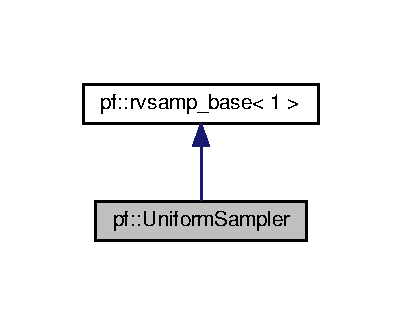
\includegraphics[width=193pt]{classpf_1_1UniformSampler__inherit__graph}
\end{center}
\end{figure}


Collaboration diagram for pf\+:\+:Uniform\+Sampler\+:\nopagebreak
\begin{figure}[H]
\begin{center}
\leavevmode
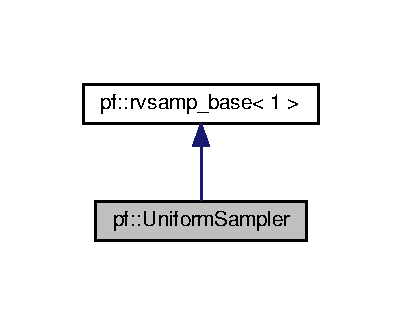
\includegraphics[width=193pt]{classpf_1_1UniformSampler__coll__graph}
\end{center}
\end{figure}
\subsection*{Public Member Functions}
\begin{DoxyCompactItemize}
\item 
\hyperlink{classpf_1_1UniformSampler_a19ca59054a12de75d1ac460603afa7a6}{Uniform\+Sampler} ()\hypertarget{classpf_1_1UniformSampler_a19ca59054a12de75d1ac460603afa7a6}{}\label{classpf_1_1UniformSampler_a19ca59054a12de75d1ac460603afa7a6}

\begin{DoxyCompactList}\small\item\em The default constructor. Gives a lower bound of 0 and upper bound of 1. \end{DoxyCompactList}\item 
\hyperlink{classpf_1_1UniformSampler_a7ed7e3301544495d8a85c34de6d2fd5e}{Uniform\+Sampler} (const double \&lower, const double \&upper)
\begin{DoxyCompactList}\small\item\em The constructor. \end{DoxyCompactList}\item 
double \hyperlink{classpf_1_1UniformSampler_ae16c03eea2a214ca31cea4446a0c3ff6}{sample} ()
\begin{DoxyCompactList}\small\item\em Draws a sample. \end{DoxyCompactList}\end{DoxyCompactItemize}
\subsection*{Private Attributes}
\begin{DoxyCompactItemize}
\item 
std\+::uniform\+\_\+real\+\_\+distribution \hyperlink{classpf_1_1UniformSampler_ab7b1466fc069e67f6b3ffa442d8dc02c}{m\+\_\+unif\+\_\+gen}\hypertarget{classpf_1_1UniformSampler_ab7b1466fc069e67f6b3ffa442d8dc02c}{}\label{classpf_1_1UniformSampler_ab7b1466fc069e67f6b3ffa442d8dc02c}

\begin{DoxyCompactList}\small\item\em makes uniform random variates \end{DoxyCompactList}\end{DoxyCompactItemize}
\subsection*{Additional Inherited Members}


\subsection{Detailed Description}
A class that performs sampling from a continuous uniform distribution. 

\begin{DoxyAuthor}{Author}
taylor 
\end{DoxyAuthor}


\subsection{Constructor \& Destructor Documentation}
\index{pf\+::\+Uniform\+Sampler@{pf\+::\+Uniform\+Sampler}!Uniform\+Sampler@{Uniform\+Sampler}}
\index{Uniform\+Sampler@{Uniform\+Sampler}!pf\+::\+Uniform\+Sampler@{pf\+::\+Uniform\+Sampler}}
\subsubsection[{\texorpdfstring{Uniform\+Sampler(const double \&lower, const double \&upper)}{UniformSampler(const double &lower, const double &upper)}}]{\setlength{\rightskip}{0pt plus 5cm}pf\+::\+Uniform\+Sampler\+::\+Uniform\+Sampler (
\begin{DoxyParamCaption}
\item[{const double \&}]{lower, }
\item[{const double \&}]{upper}
\end{DoxyParamCaption}
)}\hypertarget{classpf_1_1UniformSampler_a7ed7e3301544495d8a85c34de6d2fd5e}{}\label{classpf_1_1UniformSampler_a7ed7e3301544495d8a85c34de6d2fd5e}


The constructor. 


\begin{DoxyParams}{Parameters}
{\em lower} & the lower bound of the P\+R\+NG. \\
\hline
{\em upper} & the upper bound of the P\+R\+NG. \\
\hline
\end{DoxyParams}


\subsection{Member Function Documentation}
\index{pf\+::\+Uniform\+Sampler@{pf\+::\+Uniform\+Sampler}!sample@{sample}}
\index{sample@{sample}!pf\+::\+Uniform\+Sampler@{pf\+::\+Uniform\+Sampler}}
\subsubsection[{\texorpdfstring{sample()}{sample()}}]{\setlength{\rightskip}{0pt plus 5cm}double pf\+::\+Uniform\+Sampler\+::sample (
\begin{DoxyParamCaption}
{}
\end{DoxyParamCaption}
)}\hypertarget{classpf_1_1UniformSampler_ae16c03eea2a214ca31cea4446a0c3ff6}{}\label{classpf_1_1UniformSampler_ae16c03eea2a214ca31cea4446a0c3ff6}


Draws a sample. 

\begin{DoxyReturn}{Returns}
a sample of type double. 
\end{DoxyReturn}


The documentation for this class was generated from the following file\+:\begin{DoxyCompactItemize}
\item 
include/\hyperlink{rv__samp_8h}{rv\+\_\+samp.\+h}\end{DoxyCompactItemize}

\hypertarget{classpf_1_1UnivNormSampler}{}\section{pf\+:\+:Univ\+Norm\+Sampler Class Reference}
\label{classpf_1_1UnivNormSampler}\index{pf\+::\+Univ\+Norm\+Sampler@{pf\+::\+Univ\+Norm\+Sampler}}


A class that performs sampling from a univariate Normal distribution.  




{\ttfamily \#include $<$rv\+\_\+samp.\+h$>$}



Inheritance diagram for pf\+:\+:Univ\+Norm\+Sampler\+:\nopagebreak
\begin{figure}[H]
\begin{center}
\leavevmode
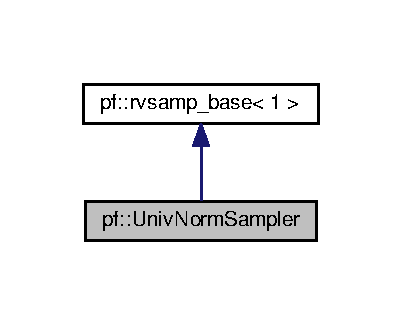
\includegraphics[width=193pt]{classpf_1_1UnivNormSampler__inherit__graph}
\end{center}
\end{figure}


Collaboration diagram for pf\+:\+:Univ\+Norm\+Sampler\+:\nopagebreak
\begin{figure}[H]
\begin{center}
\leavevmode
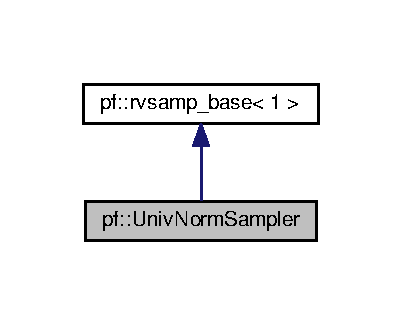
\includegraphics[width=193pt]{classpf_1_1UnivNormSampler__coll__graph}
\end{center}
\end{figure}
\subsection*{Public Member Functions}
\begin{DoxyCompactItemize}
\item 
\hyperlink{classpf_1_1UnivNormSampler_ae357a6e2e9a58cd408ffabec0e253ea1}{Univ\+Norm\+Sampler} ()\hypertarget{classpf_1_1UnivNormSampler_ae357a6e2e9a58cd408ffabec0e253ea1}{}\label{classpf_1_1UnivNormSampler_ae357a6e2e9a58cd408ffabec0e253ea1}

\begin{DoxyCompactList}\small\item\em Default-\/constructor sets up for standard Normal random variate generation. \end{DoxyCompactList}\item 
\hyperlink{classpf_1_1UnivNormSampler_a134163f5d2282415f5336f42c8f7a506}{Univ\+Norm\+Sampler} (const double \&mu, const double \&sigma)
\begin{DoxyCompactList}\small\item\em The user must supply both mean and std. dev. \end{DoxyCompactList}\item 
void \hyperlink{classpf_1_1UnivNormSampler_a62547b01925d625dfbb73fe6b37f2635}{set\+Std\+Dev} (const double \&sigma)
\begin{DoxyCompactList}\small\item\em sets the standard deviation of the sampler. \end{DoxyCompactList}\item 
void \hyperlink{classpf_1_1UnivNormSampler_a9ccf5ce6dcd9edbf51b799f3b29fff96}{set\+Mean} (const double \&mu)
\begin{DoxyCompactList}\small\item\em sets the mean of the sampler. \end{DoxyCompactList}\item 
double \hyperlink{classpf_1_1UnivNormSampler_abc3e8612cb6847516370aa4a9a5d1258}{sample} ()
\begin{DoxyCompactList}\small\item\em Draws a random number. \end{DoxyCompactList}\end{DoxyCompactItemize}
\subsection*{Private Attributes}
\begin{DoxyCompactItemize}
\item 
std\+::normal\+\_\+distribution \hyperlink{classpf_1_1UnivNormSampler_a4a8afd473ade0394b9361734743ef055}{m\+\_\+z\+\_\+gen}\hypertarget{classpf_1_1UnivNormSampler_a4a8afd473ade0394b9361734743ef055}{}\label{classpf_1_1UnivNormSampler_a4a8afd473ade0394b9361734743ef055}

\begin{DoxyCompactList}\small\item\em makes normal random variates \end{DoxyCompactList}\item 
double \hyperlink{classpf_1_1UnivNormSampler_ababec984e114e54477cbcb7ee2e87841}{m\+\_\+mu}\hypertarget{classpf_1_1UnivNormSampler_ababec984e114e54477cbcb7ee2e87841}{}\label{classpf_1_1UnivNormSampler_ababec984e114e54477cbcb7ee2e87841}

\begin{DoxyCompactList}\small\item\em the mean \end{DoxyCompactList}\item 
double \hyperlink{classpf_1_1UnivNormSampler_a1d62e630ea2386b04495dec9dce2ed95}{m\+\_\+sigma}\hypertarget{classpf_1_1UnivNormSampler_a1d62e630ea2386b04495dec9dce2ed95}{}\label{classpf_1_1UnivNormSampler_a1d62e630ea2386b04495dec9dce2ed95}

\begin{DoxyCompactList}\small\item\em the standard deviation \end{DoxyCompactList}\end{DoxyCompactItemize}
\subsection*{Additional Inherited Members}


\subsection{Detailed Description}
A class that performs sampling from a univariate Normal distribution. 

\begin{DoxyAuthor}{Author}
taylor 
\end{DoxyAuthor}


\subsection{Constructor \& Destructor Documentation}
\index{pf\+::\+Univ\+Norm\+Sampler@{pf\+::\+Univ\+Norm\+Sampler}!Univ\+Norm\+Sampler@{Univ\+Norm\+Sampler}}
\index{Univ\+Norm\+Sampler@{Univ\+Norm\+Sampler}!pf\+::\+Univ\+Norm\+Sampler@{pf\+::\+Univ\+Norm\+Sampler}}
\subsubsection[{\texorpdfstring{Univ\+Norm\+Sampler(const double \&mu, const double \&sigma)}{UnivNormSampler(const double &mu, const double &sigma)}}]{\setlength{\rightskip}{0pt plus 5cm}pf\+::\+Univ\+Norm\+Sampler\+::\+Univ\+Norm\+Sampler (
\begin{DoxyParamCaption}
\item[{const double \&}]{mu, }
\item[{const double \&}]{sigma}
\end{DoxyParamCaption}
)}\hypertarget{classpf_1_1UnivNormSampler_a134163f5d2282415f5336f42c8f7a506}{}\label{classpf_1_1UnivNormSampler_a134163f5d2282415f5336f42c8f7a506}


The user must supply both mean and std. dev. 


\begin{DoxyParams}{Parameters}
{\em mu} & a double for the mean of the sampling distribution. \\
\hline
{\em sigma} & a double ($>$ 0) representing the standard deviation of the samples. \\
\hline
\end{DoxyParams}


\subsection{Member Function Documentation}
\index{pf\+::\+Univ\+Norm\+Sampler@{pf\+::\+Univ\+Norm\+Sampler}!sample@{sample}}
\index{sample@{sample}!pf\+::\+Univ\+Norm\+Sampler@{pf\+::\+Univ\+Norm\+Sampler}}
\subsubsection[{\texorpdfstring{sample()}{sample()}}]{\setlength{\rightskip}{0pt plus 5cm}double pf\+::\+Univ\+Norm\+Sampler\+::sample (
\begin{DoxyParamCaption}
{}
\end{DoxyParamCaption}
)}\hypertarget{classpf_1_1UnivNormSampler_abc3e8612cb6847516370aa4a9a5d1258}{}\label{classpf_1_1UnivNormSampler_abc3e8612cb6847516370aa4a9a5d1258}


Draws a random number. 

\begin{DoxyReturn}{Returns}
a random sample of type double. 
\end{DoxyReturn}
\index{pf\+::\+Univ\+Norm\+Sampler@{pf\+::\+Univ\+Norm\+Sampler}!set\+Mean@{set\+Mean}}
\index{set\+Mean@{set\+Mean}!pf\+::\+Univ\+Norm\+Sampler@{pf\+::\+Univ\+Norm\+Sampler}}
\subsubsection[{\texorpdfstring{set\+Mean(const double \&mu)}{setMean(const double &mu)}}]{\setlength{\rightskip}{0pt plus 5cm}void pf\+::\+Univ\+Norm\+Sampler\+::set\+Mean (
\begin{DoxyParamCaption}
\item[{const double \&}]{mu}
\end{DoxyParamCaption}
)}\hypertarget{classpf_1_1UnivNormSampler_a9ccf5ce6dcd9edbf51b799f3b29fff96}{}\label{classpf_1_1UnivNormSampler_a9ccf5ce6dcd9edbf51b799f3b29fff96}


sets the mean of the sampler. 


\begin{DoxyParams}{Parameters}
{\em mu} & the desired mean. \\
\hline
\end{DoxyParams}
\index{pf\+::\+Univ\+Norm\+Sampler@{pf\+::\+Univ\+Norm\+Sampler}!set\+Std\+Dev@{set\+Std\+Dev}}
\index{set\+Std\+Dev@{set\+Std\+Dev}!pf\+::\+Univ\+Norm\+Sampler@{pf\+::\+Univ\+Norm\+Sampler}}
\subsubsection[{\texorpdfstring{set\+Std\+Dev(const double \&sigma)}{setStdDev(const double &sigma)}}]{\setlength{\rightskip}{0pt plus 5cm}void pf\+::\+Univ\+Norm\+Sampler\+::set\+Std\+Dev (
\begin{DoxyParamCaption}
\item[{const double \&}]{sigma}
\end{DoxyParamCaption}
)}\hypertarget{classpf_1_1UnivNormSampler_a62547b01925d625dfbb73fe6b37f2635}{}\label{classpf_1_1UnivNormSampler_a62547b01925d625dfbb73fe6b37f2635}


sets the standard deviation of the sampler. 


\begin{DoxyParams}{Parameters}
{\em sigma} & the desired standard deviation. \\
\hline
\end{DoxyParams}


The documentation for this class was generated from the following file\+:\begin{DoxyCompactItemize}
\item 
include/\hyperlink{rv__samp_8h}{rv\+\_\+samp.\+h}\end{DoxyCompactItemize}

\chapter{File Documentation}
\hypertarget{auxiliary__pf_8h}{}\section{include/auxiliary\+\_\+pf.h File Reference}
\label{auxiliary__pf_8h}\index{include/auxiliary\+\_\+pf.\+h@{include/auxiliary\+\_\+pf.\+h}}


A base class for Auxiliary Particle Filtering. Inherit from this if you want to use an \hyperlink{classAPF}{A\+PF} for your state space model. Filtering only, no smoothing.  


{\ttfamily \#include $<$array$>$}\\*
{\ttfamily \#include $<$functional$>$}\\*
{\ttfamily \#include $<$Eigen/\+Dense$>$}\\*
{\ttfamily \#include $<$cmath$>$}\\*
{\ttfamily \#include \char`\"{}rv\+\_\+samp.\+h\char`\"{}}\\*
{\ttfamily \#include $<$iostream$>$}\\*
Include dependency graph for auxiliary\+\_\+pf.\+h\+:
\nopagebreak
\begin{figure}[H]
\begin{center}
\leavevmode
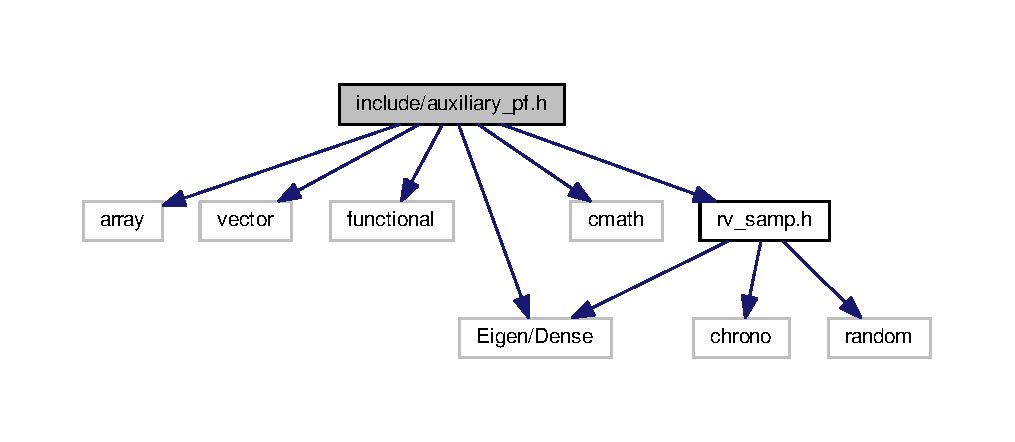
\includegraphics[width=350pt]{auxiliary__pf_8h__incl}
\end{center}
\end{figure}
\subsection*{Classes}
\begin{DoxyCompactItemize}
\item 
class \hyperlink{classAPF}{A\+P\+F$<$ nparts, dimx, dimy, resamp\+T $>$}
\begin{DoxyCompactList}\small\item\em A base-\/class for Auxiliary Particle Filtering. Filtering only, no smoothing. \end{DoxyCompactList}\end{DoxyCompactItemize}


\subsection{Detailed Description}
A base class for Auxiliary Particle Filtering. Inherit from this if you want to use an \hyperlink{classAPF}{A\+PF} for your state space model. Filtering only, no smoothing. 


\begin{DoxyTemplParams}{Template Parameters}
{\em nparts} & the number of particles \\
\hline
{\em dimx} & the dimension of the state \\
\hline
{\em dimy} & the dimension of the observations \\
\hline
{\em resampT} & the resampler type \\
\hline
\end{DoxyTemplParams}

\hypertarget{bootstrap__filter_8h}{}\section{include/pf/bootstrap\+\_\+filter.h File Reference}
\label{bootstrap__filter_8h}\index{include/pf/bootstrap\+\_\+filter.\+h@{include/pf/bootstrap\+\_\+filter.\+h}}


bootstrap particle filter  


{\ttfamily \#include $<$array$>$}\newline
{\ttfamily \#include $<$vector$>$}\newline
{\ttfamily \#include $<$Eigen/\+Dense$>$}\newline
{\ttfamily \#include \char`\"{}pf\+\_\+base.\+h\char`\"{}}\newline
Include dependency graph for bootstrap\+\_\+filter.\+h\+:\nopagebreak
\begin{figure}[H]
\begin{center}
\leavevmode
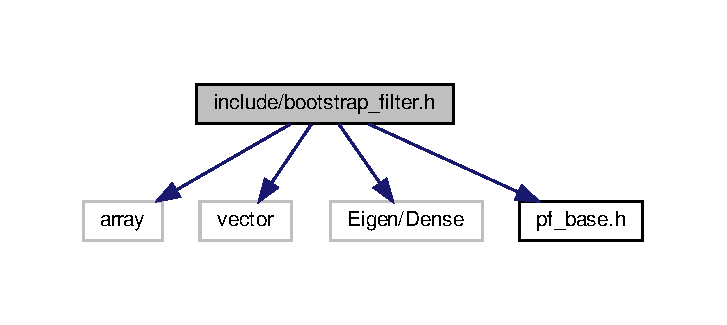
\includegraphics[width=350pt]{bootstrap__filter_8h__incl}
\end{center}
\end{figure}
\subsection*{Classes}
\begin{DoxyCompactItemize}
\item 
class \hyperlink{classBSFilter}{B\+S\+Filter$<$ nparts, dimx, dimy, resamp\+\_\+t, float\+\_\+t, debug $>$}
\begin{DoxyCompactList}\small\item\em A base class for the bootstrap particle filter. \end{DoxyCompactList}\end{DoxyCompactItemize}


\subsection{Detailed Description}
bootstrap particle filter 


\begin{DoxyTemplParams}{Template Parameters}
{\em nparts} & the number of particles \\
\hline
{\em dimx} & the dimension of the state \\
\hline
{\em dimy} & the dimension of the observations \\
\hline
{\em resamp\+\_\+t} & the type of resampler \\
\hline
\end{DoxyTemplParams}

\hypertarget{cf__filters_8h}{}\section{include/cf\+\_\+filters.h File Reference}
\label{cf__filters_8h}\index{include/cf\+\_\+filters.\+h@{include/cf\+\_\+filters.\+h}}


forces structure on the closed-\/form filters.  


{\ttfamily \#include $<$Eigen/\+Dense$>$}\newline
{\ttfamily \#include $<$math.\+h$>$}\newline
{\ttfamily \#include \char`\"{}rv\+\_\+eval.\+h\char`\"{}}\newline
Include dependency graph for cf\+\_\+filters.\+h\+:\nopagebreak
\begin{figure}[H]
\begin{center}
\leavevmode
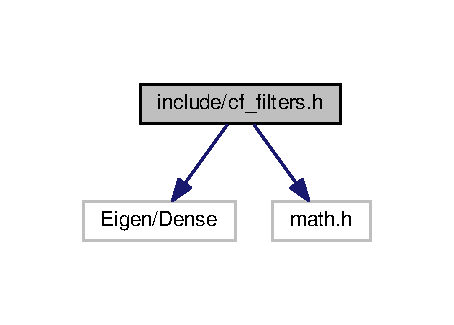
\includegraphics[width=350pt]{cf__filters_8h__incl}
\end{center}
\end{figure}
This graph shows which files directly or indirectly include this file\+:\nopagebreak
\begin{figure}[H]
\begin{center}
\leavevmode
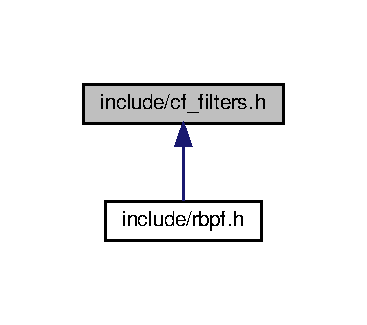
\includegraphics[width=176pt]{cf__filters_8h__dep__incl}
\end{center}
\end{figure}
\subsection*{Classes}
\begin{DoxyCompactItemize}
\item 
class \hyperlink{classcf__filter}{cf\+\_\+filter$<$ dimstate, dimobs, float\+\_\+t $>$}
\begin{DoxyCompactList}\small\item\em Abstract Base Class for all closed-\/form filters. \end{DoxyCompactList}\item 
class \hyperlink{classkalman}{kalman$<$ dimstate, dimobs, diminput, float\+\_\+t $>$}
\begin{DoxyCompactList}\small\item\em A class template for Kalman filtering. \end{DoxyCompactList}\item 
class \hyperlink{classhmm}{hmm$<$ dimstate, dimobs, float\+\_\+t $>$}
\begin{DoxyCompactList}\small\item\em A class template for H\+MM filtering. \end{DoxyCompactList}\item 
class \hyperlink{classgamFilter}{gam\+Filter$<$ dim\+\_\+pred, float\+\_\+t $>$}
\begin{DoxyCompactList}\small\item\em A class template for Gamma filtering. \end{DoxyCompactList}\item 
class \hyperlink{classmultivGamFilter}{multiv\+Gam\+Filter$<$ dim\+\_\+obs, dim\+\_\+pred, float\+\_\+t $>$}
\begin{DoxyCompactList}\small\item\em Another class template for Gamma filtering, but this time. \end{DoxyCompactList}\end{DoxyCompactItemize}


\subsection{Detailed Description}
forces structure on the closed-\/form filters. 

Inherit from this for a model that admits Gamma filtering.

Inherit from this for a model that admits H\+MM filtering.

Inherit from this for a model that admits Kalman filtering.
\hypertarget{resamplers_8h}{}\section{include/pf/resamplers.h File Reference}
\label{resamplers_8h}\index{include/pf/resamplers.\+h@{include/pf/resamplers.\+h}}


all resamplers must inherit from this. This will enforce certain structure that are assumed by all particle filters.  


{\ttfamily \#include $<$chrono$>$}\newline
{\ttfamily \#include $<$array$>$}\newline
{\ttfamily \#include $<$random$>$}\newline
{\ttfamily \#include $<$numeric$>$}\newline
{\ttfamily \#include $<$cmath$>$}\newline
{\ttfamily \#include $<$Eigen/\+Dense$>$}\newline
Include dependency graph for resamplers.\+h\+:
\nopagebreak
\begin{figure}[H]
\begin{center}
\leavevmode
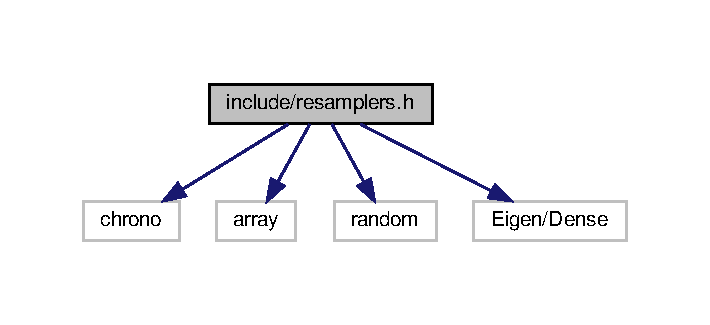
\includegraphics[width=350pt]{resamplers_8h__incl}
\end{center}
\end{figure}
\subsection*{Classes}
\begin{DoxyCompactItemize}
\item 
class \hyperlink{classrbase}{rbase$<$ nparts, dimx, float\+\_\+t $>$}
\begin{DoxyCompactList}\small\item\em Base class for all resampler types. \end{DoxyCompactList}\item 
class \hyperlink{classmn__resampler}{mn\+\_\+resampler$<$ nparts, dimx, float\+\_\+t $>$}
\item 
class \hyperlink{classmn__resampler__rbpf}{mn\+\_\+resampler\+\_\+rbpf$<$ nparts, dimsampledx, cf\+Mod\+T, float\+\_\+t $>$}
\item 
class \hyperlink{classresid__resampler}{resid\+\_\+resampler$<$ nparts, dimx, float\+\_\+t $>$}
\item 
class \hyperlink{classstratif__resampler}{stratif\+\_\+resampler$<$ nparts, dimx, float\+\_\+t $>$}
\item 
class \hyperlink{classsystematic__resampler}{systematic\+\_\+resampler$<$ nparts, dimx, float\+\_\+t $>$}
\item 
class \hyperlink{classmn__resamp__fast1}{mn\+\_\+resamp\+\_\+fast1$<$ nparts, dimx, float\+\_\+t $>$}
\end{DoxyCompactItemize}


\subsection{Detailed Description}
all resamplers must inherit from this. This will enforce certain structure that are assumed by all particle filters. 

Class that performs multinomial resampling for \char`\"{}standard\char`\"{} models. For justification, see page 244 of \char`\"{}\+Inference in Hidden Markov Models\char`\"{}.

Class that performs systematic resampling on \char`\"{}standard\char`\"{} models.

Class that performs stratified resampling on \char`\"{}standard\char`\"{} models.

Class that performs residual resampling on \char`\"{}standard\char`\"{} models.

Class that performs multinomial resampling for R\+B\+P\+Fs.

Class that performs multinomial resampling for \char`\"{}standard\char`\"{} models.


\begin{DoxyTemplParams}{Template Parameters}
{\em nparts} & the number of particles. \\
\hline
{\em dimx} & the dimension of each state sample.\\
\hline
{\em nparts} & the number of particles. \\
\hline
{\em dimsampledx} & the dimension of each state sample. \\
\hline
{\em cf\+ModT} & the type of closed form model \\
\hline
{\em float\+\_\+t} & the type of floating point number\\
\hline
{\em nparts} & the number of particles. \\
\hline
{\em dimx} & the dimension of each state sample. \\
\hline
{\em float\+\_\+t} & the floating point for samples \\
\hline
\end{DoxyTemplParams}

\hypertarget{rv__samp_8h}{}\section{include/pf/rv\+\_\+samp.h File Reference}
\label{rv__samp_8h}\index{include/pf/rv\+\_\+samp.\+h@{include/pf/rv\+\_\+samp.\+h}}


all rv samplers must inherit from this.  


{\ttfamily \#include $<$chrono$>$}\newline
{\ttfamily \#include $<$Eigen/\+Dense$>$}\newline
{\ttfamily \#include $<$random$>$}\newline
Include dependency graph for rv\+\_\+samp.\+h\+:
\nopagebreak
\begin{figure}[H]
\begin{center}
\leavevmode
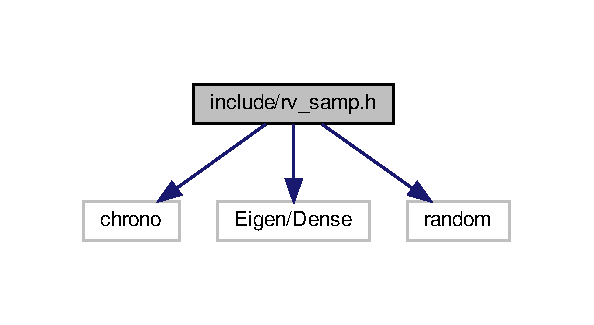
\includegraphics[width=285pt]{rv__samp_8h__incl}
\end{center}
\end{figure}
This graph shows which files directly or indirectly include this file\+:
\nopagebreak
\begin{figure}[H]
\begin{center}
\leavevmode
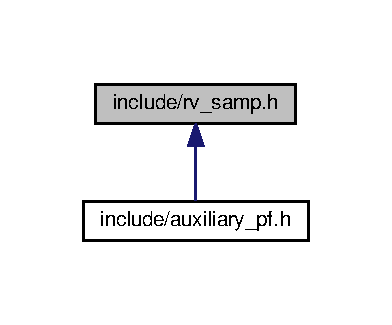
\includegraphics[width=199pt]{rv__samp_8h__dep__incl}
\end{center}
\end{figure}
\subsection*{Classes}
\begin{DoxyCompactItemize}
\item 
class \hyperlink{classrvsamp_1_1rvsamp__base}{rvsamp\+::rvsamp\+\_\+base}
\begin{DoxyCompactList}\small\item\em Base class for all random variable sampler types. Primary benefit is that it sets the seed for you. \end{DoxyCompactList}\item 
class \hyperlink{classrvsamp_1_1UnivNormSampler}{rvsamp\+::\+Univ\+Norm\+Sampler$<$ float\+\_\+t $>$}
\begin{DoxyCompactList}\small\item\em A class that performs sampling from a univariate Normal distribution. \end{DoxyCompactList}\item 
class \hyperlink{classrvsamp_1_1UnivLogNormSampler}{rvsamp\+::\+Univ\+Log\+Norm\+Sampler$<$ float\+\_\+t $>$}
\begin{DoxyCompactList}\small\item\em A class that performs sampling from a univariate Log-\/\+Normal distribution. \end{DoxyCompactList}\item 
class \hyperlink{classrvsamp_1_1UnivGammaSampler}{rvsamp\+::\+Univ\+Gamma\+Sampler$<$ float\+\_\+t $>$}
\begin{DoxyCompactList}\small\item\em A class that performs sampling from a univariate Gamma distribution. \end{DoxyCompactList}\item 
class \hyperlink{classrvsamp_1_1UnivInvGammaSampler}{rvsamp\+::\+Univ\+Inv\+Gamma\+Sampler$<$ float\+\_\+t $>$}
\begin{DoxyCompactList}\small\item\em A class that performs sampling from a univariate Inverse Gamma distribution. \end{DoxyCompactList}\item 
class \hyperlink{classrvsamp_1_1TruncUnivNormSampler}{rvsamp\+::\+Trunc\+Univ\+Norm\+Sampler$<$ float\+\_\+t $>$}
\begin{DoxyCompactList}\small\item\em A class that performs sampling from a truncated univariate Normal distribution. \end{DoxyCompactList}\item 
class \hyperlink{classrvsamp_1_1PoissonSampler}{rvsamp\+::\+Poisson\+Sampler$<$ float\+\_\+t, int\+\_\+t $>$}
\begin{DoxyCompactList}\small\item\em A class that performs sampling from a Poisson distribution. \end{DoxyCompactList}\item 
class \hyperlink{classrvsamp_1_1BernSampler}{rvsamp\+::\+Bern\+Sampler$<$ float\+\_\+t, int\+\_\+t $>$}
\begin{DoxyCompactList}\small\item\em A class that performs sampling from a univariate Bernoulli distribution. \end{DoxyCompactList}\item 
class \hyperlink{classrvsamp_1_1MVNSampler}{rvsamp\+::\+M\+V\+N\+Sampler$<$ dim, float\+\_\+t $>$}
\begin{DoxyCompactList}\small\item\em A class that performs sampling from a multivariate normal distribution. \end{DoxyCompactList}\item 
class \hyperlink{classrvsamp_1_1UniformSampler}{rvsamp\+::\+Uniform\+Sampler$<$ float\+\_\+t $>$}
\begin{DoxyCompactList}\small\item\em A class that performs sampling from a continuous uniform distribution. \end{DoxyCompactList}\item 
class \hyperlink{classrvsamp_1_1k__gen}{rvsamp\+::k\+\_\+gen$<$ N, float\+\_\+t $>$}
\begin{DoxyCompactList}\small\item\em A class that performs sampling with replacement (useful for the index sampler in an \hyperlink{classAPF}{A\+PF}) \end{DoxyCompactList}\end{DoxyCompactItemize}


\subsection{Detailed Description}
all rv samplers must inherit from this. 

Basically a wrapper for std\+::discrete\+\_\+distribution$<$$>$ outputs are in the rage (0,1,...N-\/1)

Can sample from a distribution with fixed mean and covariance, fixed mean only, fixed covariance only, or nothing fixed.

Samples from univariate Bernoulli distribution.

Samples from univariate Poisson distribution.

Samples from a truncated univariate Normal distribution using the acceptance rejection method. The proposal distribution used is a normal distribution with the same location and scale parameters as the target. As a result, this method will take a long time when the width of the support of the target is narrow.

Samples from univariate Inverse Gamma distribution.

Samples from univariate Gamma distribution.

Samples from univariate Log-\/\+Normal distribution.

Samples from univariate Normal distribution.


\begin{DoxyTemplParams}{Template Parameters}
{\em dim} & the dimension of each random vector sample.\\
\hline
\end{DoxyTemplParams}

\hypertarget{sisr__filter_8h}{}\section{include/pf/sisr\+\_\+filter.h File Reference}
\label{sisr__filter_8h}\index{include/pf/sisr\+\_\+filter.\+h@{include/pf/sisr\+\_\+filter.\+h}}


S\+I\+SR filter.  


{\ttfamily \#include $<$array$>$}\newline
{\ttfamily \#include $<$Eigen/\+Dense$>$}\newline
{\ttfamily \#include \char`\"{}pf\+\_\+base.\+h\char`\"{}}\newline
Include dependency graph for sisr\+\_\+filter.\+h\+:\nopagebreak
\begin{figure}[H]
\begin{center}
\leavevmode
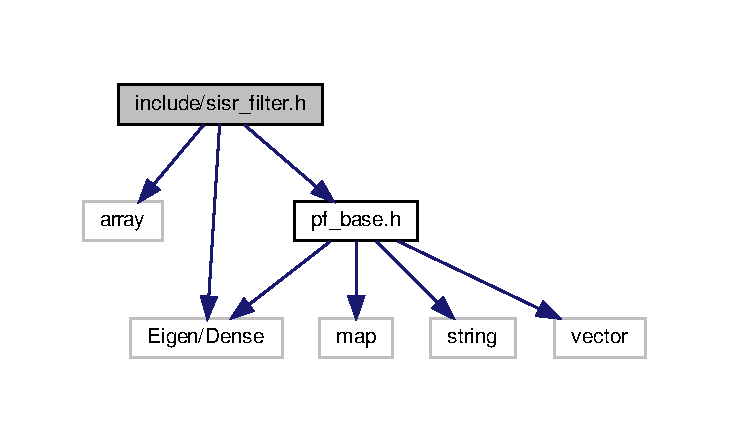
\includegraphics[width=350pt]{sisr__filter_8h__incl}
\end{center}
\end{figure}
\subsection*{Classes}
\begin{DoxyCompactItemize}
\item 
class \hyperlink{classSISRFilter}{S\+I\+S\+R\+Filter$<$ nparts, dimx, dimy, resamp\+\_\+t, float\+\_\+t, debug $>$}
\begin{DoxyCompactList}\small\item\em A base class for the Sequential Important Sampling with Resampling (S\+I\+SR). \end{DoxyCompactList}\end{DoxyCompactItemize}


\subsection{Detailed Description}
S\+I\+SR filter. 


\begin{DoxyTemplParams}{Template Parameters}
{\em nparts} & the number of particles \\
\hline
{\em dimx} & the size of the state \\
\hline
{\em the} & size of the observation \\
\hline
{\em resamp\+\_\+t} & the type of resampler \\
\hline
\end{DoxyTemplParams}

%--- End generated contents ---

% Index
\backmatter
\newpage
\phantomsection
\clearemptydoublepage
\addcontentsline{toc}{chapter}{Index}
\printindex

\end{document}
